\documentclass[titlepage]{tufte-book}

\usepackage[runall=true]{pythontex}
\usepackage{environ}
\usepackage{morewrites}
\usepackage{amsthm}
\usepackage{amsmath}
\usepackage{amssymb}
\usepackage[pdftex]{graphicx}
\usepackage{epstopdf}
\usepackage{hyperref}
\usepackage{alltt}
\usepackage{listings}
\usepackage{array}
\usepackage{extarrows}
\usepackage{setspace}
\usepackage{tikz}
\usepackage{tikz-qtree}
\usetikzlibrary{calc}
\usetikzlibrary{positioning}
\usepackage{hyperref}
\usepackage{graphviz}
\usepackage{geometry}                % See geometry.pdf to learn the layout options. There are lots.
\usepackage{bashful}
\usepackage{microtype} % Improves character and word spacing
\usepackage{caption}

\usepackage{booktabs} % Better horizontal rules in tables

\setkeys{Gin}{width=\linewidth,totalheight=\textheight,keepaspectratio} % Improves figure scaling
\graphicspath{{figures/}}

\usepackage{fancyvrb} % Allows customization of verbatim environments
\fvset{fontsize=\normalsize} % The font size of all verbatim text can be changed here

\newcounter{problem}
\newcounter{total}
\newcommand{\step}[1]{{}
\vspace{4pt} \noindent {\bf \theproblem. }#1\addtocounter{problem}{1}}

\newcommand{\cut}[1]{}

\usepackage[tikz]{bclogo}
\usepackage{tikz}
\usetikzlibrary{calc}

\lstdefinestyle{BashInputStyle}{
  language=bash,
  basicstyle=\small\ttfamily,
  numberstyle=\tiny,
  showstringspaces=false,
  numbersep=3pt,
  otherkeywords={|, ;, ', ", *,>, <, *, &, `, $},
  alsoletter={:~_},
  columns=fullflexible,
  backgroundcolor=\color{yellow!20},
  linewidth=0.93\linewidth,
  xleftmargin=0.03\linewidth,
  keywordstyle=\color{blue},
  emph={ls, cat, head, tail, more, less, sort, uniq, kill java, grep, zip, unzip, tar, wc, cp, chmod,chown},
  emphstyle=\color{black}\bfseries,
    commentstyle=\color{gray}\slshape
    }

\newcommand{\chili}{\scalebox{.04}{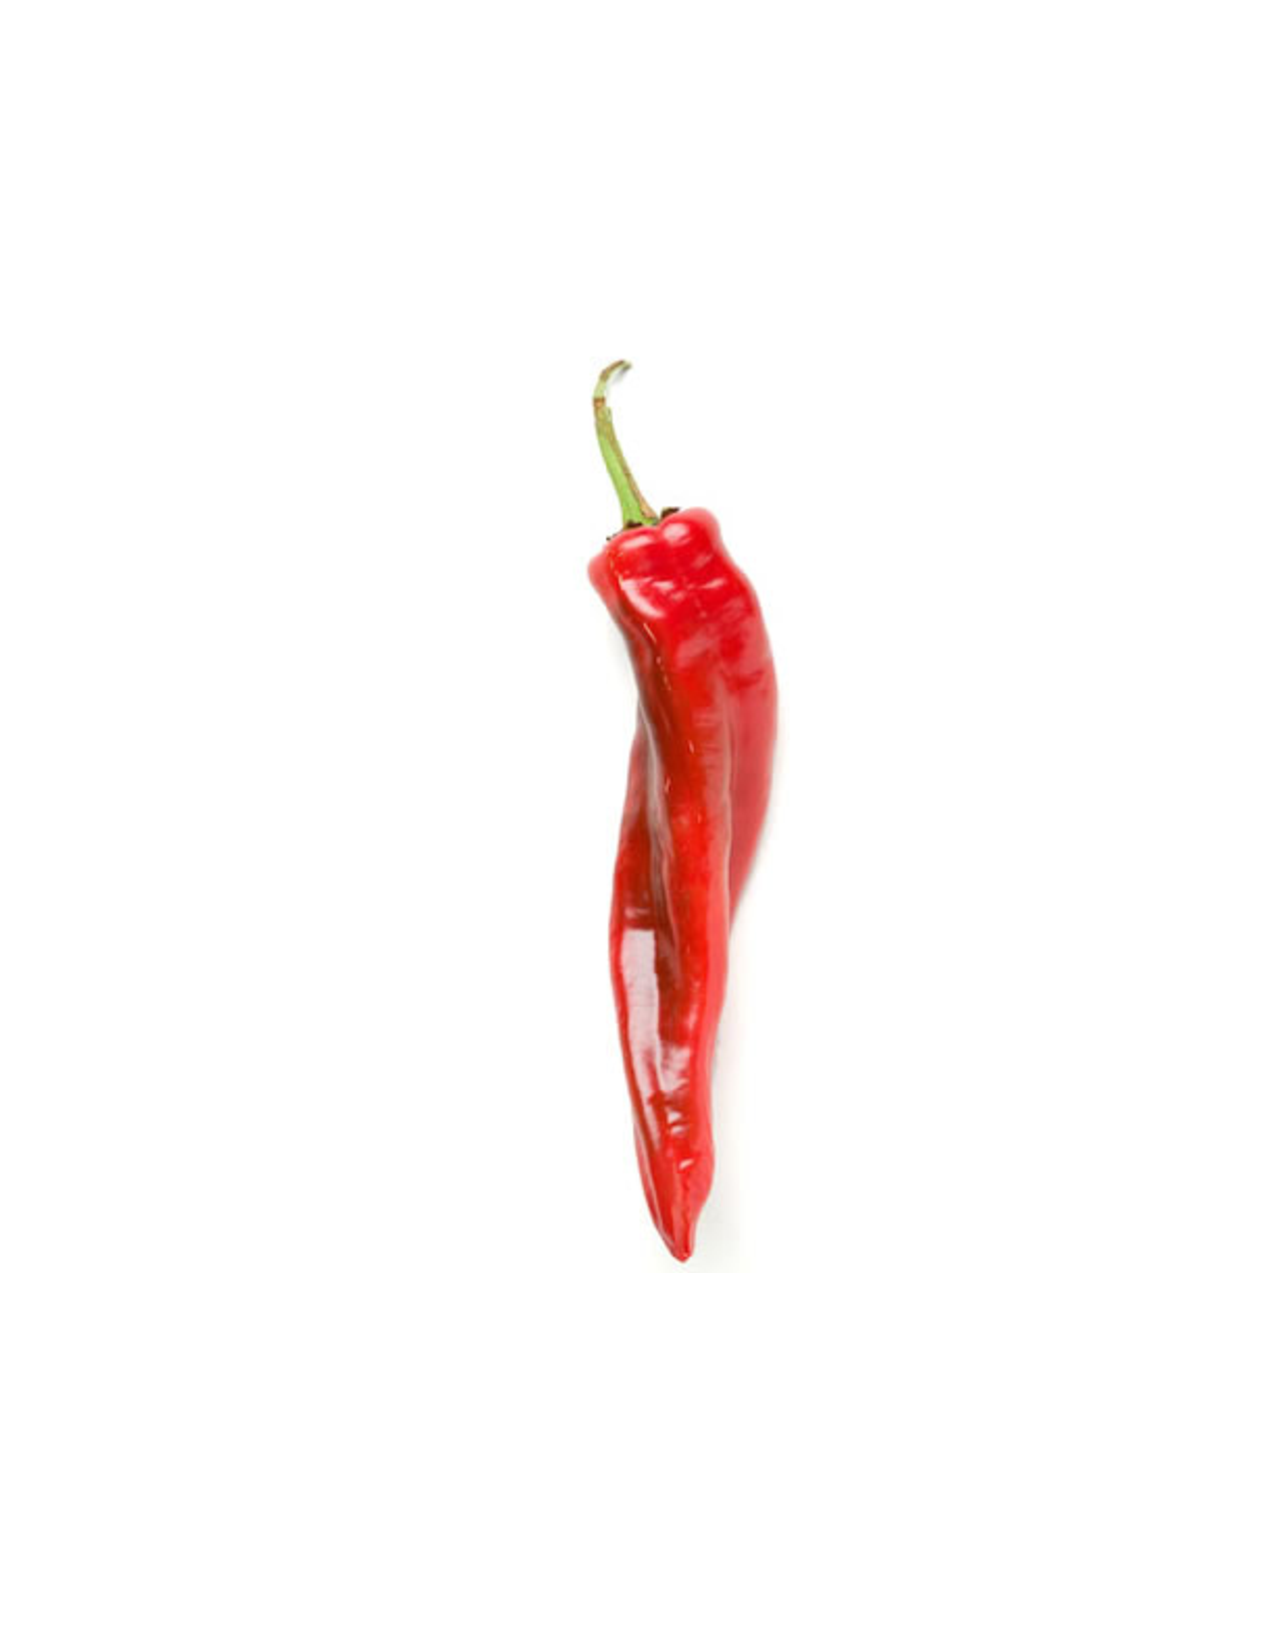
\includegraphics{figures/chili.pdf}}}
\newcommand{\chchili}{{\chili\chili}}
\newcommand{\chchchili}{{\chchili\chili}}

% The units package provides nice, non-stacked fractions and better spacing
% for units.
\usepackage{units}

% The fancyvrb package lets us customize the formatting of verbatim
% environments.  We use a slightly smaller font.
\usepackage{fancyvrb}
\fvset{fontsize=\normalsize}

% Small sections of multiple columns
\usepackage{multicol}

\hypersetup{
urlcolor=blue,
colorlinks=true
}
\usepackage[noline, procnumbered, linesnumberedhidden, boxed]{algorithm2e}

\newcommand{\openepigraph}[2]{ % This block sets up a command for printing an epigraph with 2 arguments - the quote and the author
\begin{fullwidth}
\sffamily\large
\begin{doublespace}
\noindent\allcaps{#1}\\ % The quote
\noindent\allcaps{#2} % The author
\end{doublespace}
\end{fullwidth}
}

\newcommand{\figref}[1]{Figure~\ref{#1}}

\newenvironment{callout}[1]{
\[
  \left[
      \begin{tabular}{@{\quad}m{.05\textwidth}@{\qquad}m{.75\textwidth}@{\quad}}
        \scalebox{1.5}{#1} & 
          \raggedright%
}
{
      \end{tabular}
    \right]
\]
}

\newcommand{\blankpage}{\newpage\hbox{}\thispagestyle{empty}\newpage} % Command to insert a blank page

\usepackage{makeidx} % Used to generate the index
\makeindex % Generate the index which is printed at the end of the document

\renewcommand{\maketitlepage}[0]{%
  \cleardoublepage%
  {%
  \sffamily%
  \begin{fullwidth}%
  ~
  \vspace{11.5pc}%
  \fontsize{36}{40}\selectfont\par\noindent\textcolor{darkgray}{\allcaps{\thanklesstitle}}%
  
\scalebox{.2}{
\includegraphics{figures/msan-logo}}
  \vspace{11.5pc}%
  \fontsize{12}{18}\selectfont\par\indent\textcolor{darkgray}{\allcaps{\thanklessauthor}\\
\indent{\tt parrt@cs.usfca.edu}\\
\href{http://parrt.cs.usfca.edu}{http://parrt.cs.usfca.edu}}%
  \vspace{11.5pc}%
  \fontsize{14}{16}\selectfont\par\noindent\allcaps{\thanklesspublisher}%
  \end{fullwidth}%
  }
  \thispagestyle{empty}%
  \clearpage%
}

\titlecontents{part}% FIXME
    [0em] % distance from left margin
    {\vspace{1.5\baselineskip}\begin{fullwidth}\LARGE\rmfamily\itshape} % above (global formatting of entry)
    {\contentslabel{2em}} % before w/label (label = ``II'')
    {} % before w/o label
    {\rmfamily\upshape\qquad\thecontentspage} % filler + page (leaders and page num)
    [\end{fullwidth}] % after

  \titlecontents{chapter}%
    [0em] % distance from left margin
    {\vspace{1.5\baselineskip}\begin{fullwidth}\Large\rmfamily\itshape} % above (global formatting of entry)
    {\hspace*{0em}\contentslabel{2em}} % before w/label (label = ``2'')
    {\hspace*{4em}} % before w/o label
    {\rmfamily\upshape\qquad\thecontentspage} % filler + page (leaders and page num)
    [\end{fullwidth}] % after

\titlespacing*{\chapter}{0pt}{0pt}{30pt}
\titlespacing*{\section}{0pt}{3.5ex plus 1ex minus .2ex}{2.3ex plus .2ex}
\titlespacing*{\subsection}{0pt}{3.25ex plus 1ex minus .2ex}{1.5ex plus.2ex}

\title{
Exercises in\\
Computational\\
Analytics
}

% preparatory, introductory, foundations, preliminary, survey
\author{Terence Parr}

\date{} % delete this line to display the current date

%\setcounter{secnumdepth}{0}

\begin{document}

\frontmatter

%----------------------------------------------------------------------------------------

\maketitle % Print the title page

%----------------------------------------------------------------------------------------
%	COPYRIGHT PAGE
%----------------------------------------------------------------------------------------

\newpage
\begin{fullwidth}
~\vfill
\thispagestyle{empty}
\setlength{\parindent}{0pt}
\setlength{\parskip}{\baselineskip}
Copyright \copyright\ \the\year\ Terence Parr

\par\smallcaps{A Bonkers the Cat Production}

\vspace{-5pt}
\scalebox{.15}{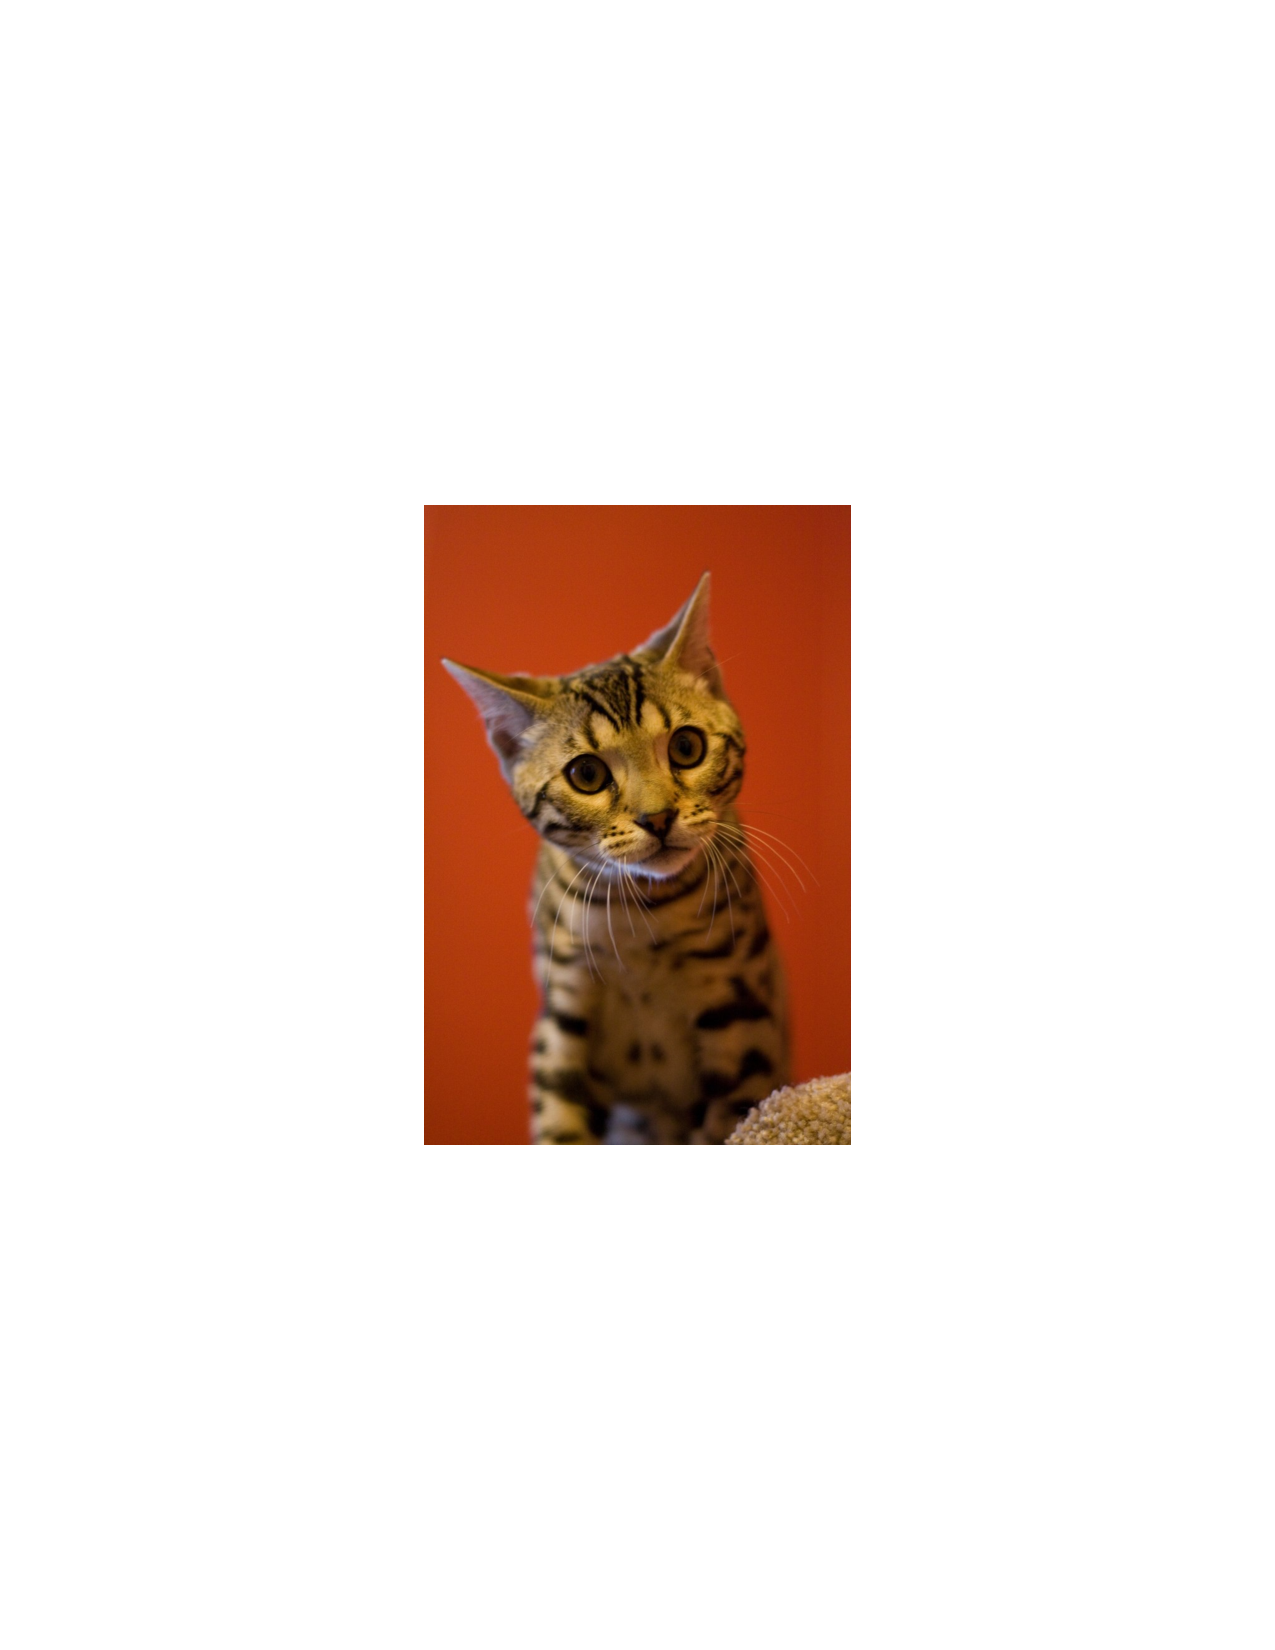
\includegraphics{figures/bonkers}}

\end{fullwidth}

%----------------------------------------------------------------------------------------

\tableofcontents % Print the table of contents

\mainmatter

\part{Introduction}

\chapter{Audience and Summary}

\newthought{Welcome to MSAN501}, the computational analytics boot camp at the University of San Francisco! This exercise book collects all of the labs you must complete by the end of the boot camp in order to pass.  The labs start out as very simple tasks or step-by-step recipes but then accelerate in difficulty, culminating with an interesting text analysis project. You will build all projects in Python (2.7.x).

\marginnote[-1in]{As you progress through these exercises, you'll learn a great deal about Python and the following libraries: {\tt matplotlib}, {\tt numpy}, {\tt scipy}, and {\tt py.test}. You'll also learn how to run jobs on computers in the cloud.}

This course is specifically designed as an introduction to analytics programming for those who are not yet skilled programmers. The course also explores many concepts from math and statistics, but in an empirical fashion rather than symbolically as one would do in a math class. Consequently, this course is also useful to programmers who'd like to strengthen their understanding of numerical methods.

\marginnote[-1in]{
\begin{center}
\scalebox{.65}{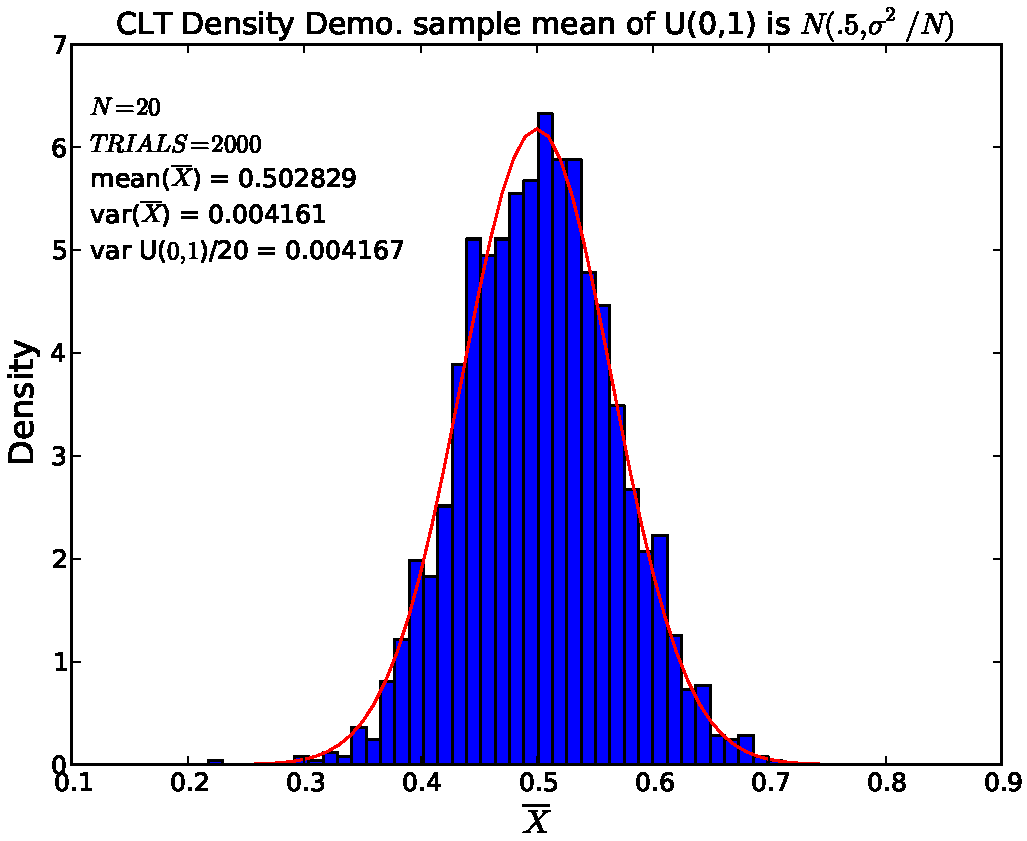
\includegraphics{figures/clt_unif-2000-20.pdf}}
\scalebox{.65}{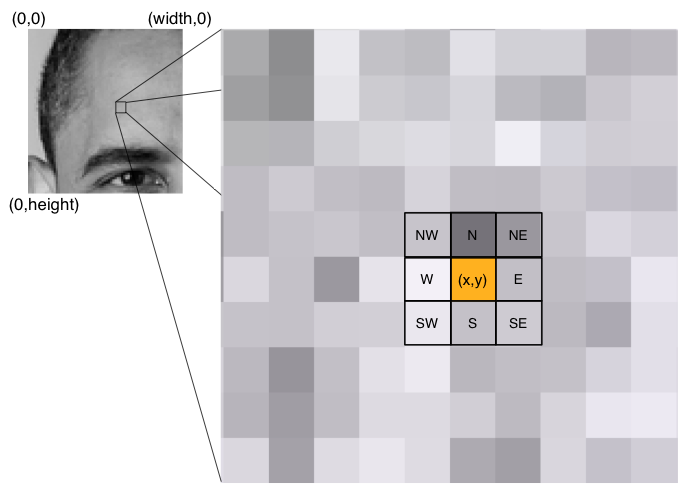
\includegraphics{figures/region.png}}\\
\scalebox{.35}{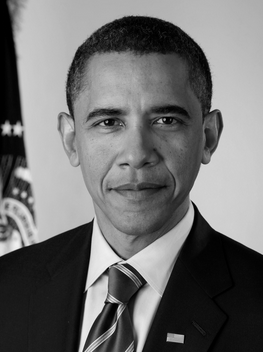
\includegraphics{figures/obama.png}}
\scalebox{.35}{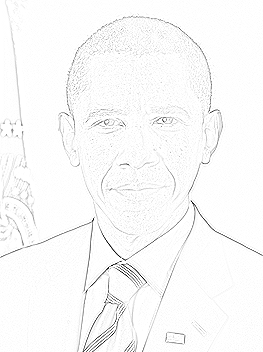
\includegraphics{figures/obama-negative-edges}}
\scalebox{.65}{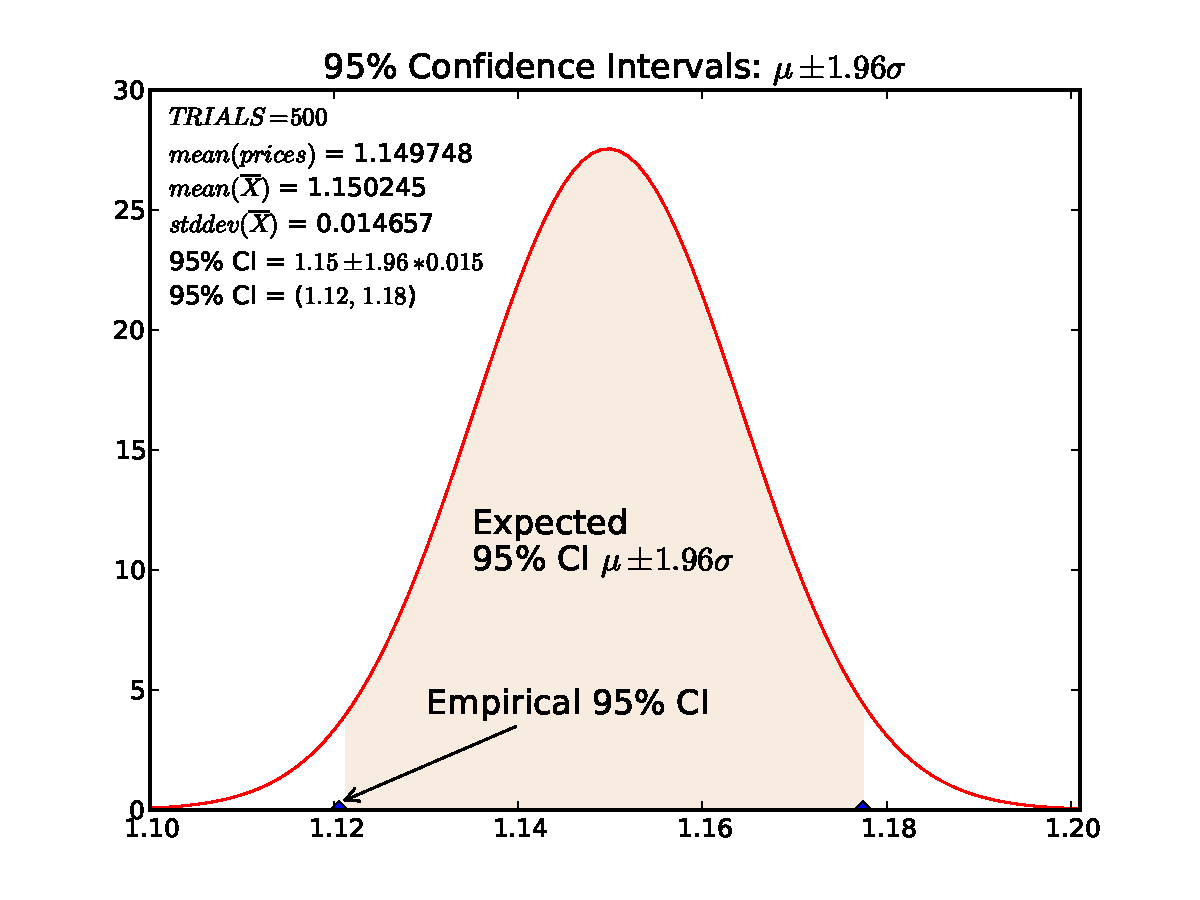
\includegraphics{figures/conf-500.pdf}}
\scalebox{.65}{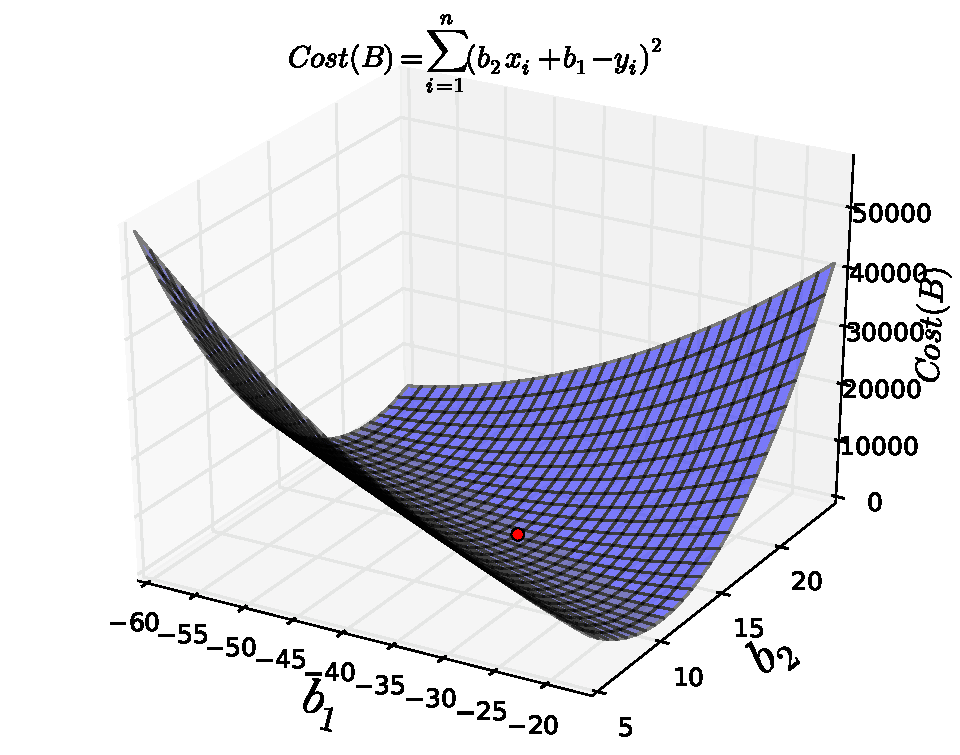
\includegraphics{figures/wage-murders-cost-3d.pdf}}
\scalebox{.65}{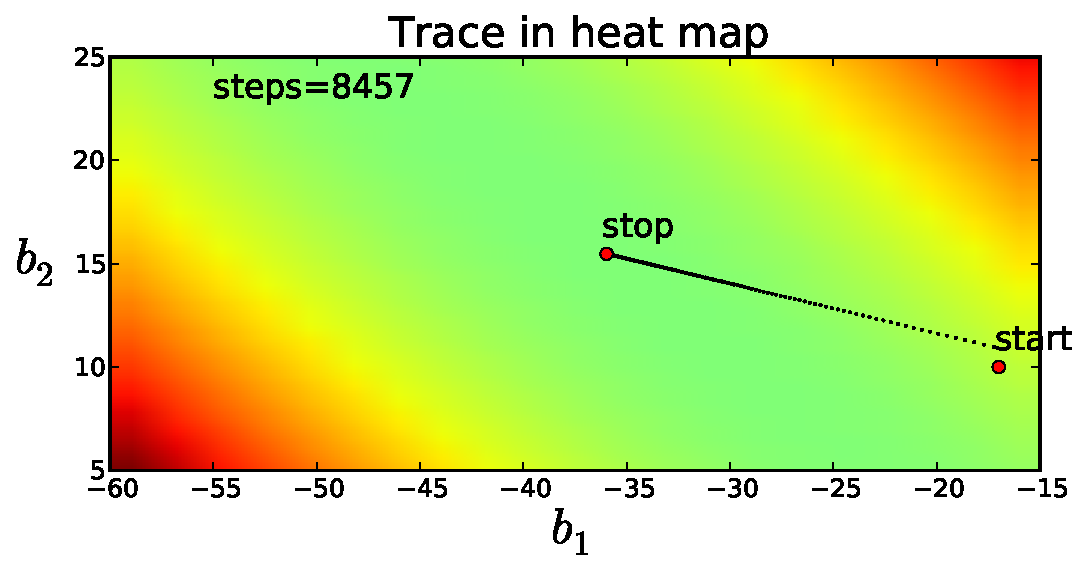
\includegraphics{figures/wage-murders-heatmap-trace1.pdf}}
\end{center}
}

The exercises are grouped into multiple parts. We begin by looking at our fundamental tools, such as the command line and PyCharm. Then we'll study how computers represent data and images, learn simple data structures, and build some visualizations. Next, we'll study how to solve a number of math and statistics problems related to analytics. The empirical statistics part strives to give an intuitive feel for random variables, density functions, the central limit theorem, hypothesis testing, and confidence intervals. It's one thing to learn about their formal definitions, but to get a really solid grasp of these concepts, it really helps to observe statistics in action. All of the techniques we'll use in empirical statistics rely on the ability to generate random values from a particular distribution. We can do it all from a uniform random number generator.

The next set of exercises deal with function optimization. Given a particular function, $f(x)$, optimizing it generally means finding its minimum or maximum, which occur when the derivative goes flat: $f'(x) = 0$. When the function's derivative cannot be derived symbolically, we're left with a general technique called {\em gradient descent} that searches for minima.

Next, you'll get an introduction to text analysis. We will compute something called {\em TFIDF} that indicates how well that word distinguishes a document from other documents in a corpus.  That score is used broadly in text analytics.

Finally, we'll launch some machines in the cloud and perform some small distributed computing tasks using hadoop and Python.

\part{Fundamental Tools}

\chapter{Linux command line}

\setcounter{problem}{1}

\begin{fullwidth}

UNIX shell is an interactive domain specific language used to control and monitor the UNIX operating system, which includes processes, devices, ram, cpus, disks etc.   It is also a programming language, though we'll use it mostly to do scripting: lists of commands. If you have to use a Windows machine, the shell is useless so try to install a UNIX shell.

\section{Everything is a stream}

The first thing you need to know is that UNIX is based upon the idea of a stream. Everything is a stream, or appears to be. Device drivers look like streams, terminals look like streams, processes communicate via streams, etc... The input and output of a program are streams that you can redirect into a device, a file, or another program.

Here is an example device, the null device, that lets you throw output away. For example, you might want to run a program but ignore the output.

\begin{alltt}\small
$ ls > /dev/null # ignore output of ls
\end{alltt}

\noindent where "\# ignore output of ls" is a comment.

Most of the commands covered in this lecture process stdin and send results to stdout. In this manner, you can incrementally process a data stream by hooking the output of one tool to the input of another via a pipe. For example, the following piped sequence prints the number of files in the current directory modified in August.

\begin{alltt}\small
$ ls -l | grep Aug | wc -l
\end{alltt}

Imagine how long it would take you to write the equivalent C or Java program. You can become an extremely productive UNIX programmer if you learn to combine the simple command-line tools.

\section{The basics}

UNIX disk structure: http://www.thegeekstuff.com/2010/09/linux-file-system-structure/

{\tt \verb|~|parrt} is my home directory, {\tt /home/parrt}, as is {\tt \verb|~|}.

{\small
\bash[script,stdout, prefix=$]
ls /
\END
}

Like when were typing in the Python shell, each command is terminated by newline. The first thing we type is the command followed by parameters (separated by whitespace):

\begin{alltt}
$ foo arg1 arg2 ... argN
\end{alltt}

That is why whitespace in filenames sucks:

\begin{alltt}\small
$ ls house\textbackslash of\textbackslash pancakes
\end{alltt}

\noindent But we can use this:

\begin{alltt}
$ ls 'house of pancakes'
\end{alltt}

The commands can be built into the shell or they can be programs that we write and invoke.  For example, here's how you ask which program is being executed when you type a command:

{\small
\bash[script,stdout,prefix=$]
which ls python
\END
}

The Python interpreter is a program installed on our disk and when we say {\tt python} at the shell, it finds the program using an ordered list of directories in {\tt PATH} environment variable and executes it.

Next, we pass information around using streams and we can shunt that data into a file or pull data from a file using special operators. You can pretend these are like operators in a programming language like addition and multiplication. Each program has standard input, standard output, and standard error; three streams. 

We can set the standard input of a process using > character:

{\small
\bash[script,stdout,prefix=$]
ls / > /tmp/foo
\END
}

Here is how to type something directly into a text file:
 
\begin{alltt}
cat > /tmp/foo
the first line of the file
the second line of the file
^D
$ 
\end{alltt}

\noindent The {\tt \^{}D} means control-D, which means end of file.  {\tt cat} is reading from standard input and writing to the file. The way it knows we are done is when we signal in the file with control-D.

We can set the standard input of a process to the contents of a file and redirect the output of a process to a file.

{\small
\bash[script,stdout,prefix=$]
wc < /tmp/foo
\END
}

or

{\small
\bash[script,stdout,prefix=$]
wc /tmp/foo
\END
}

We can connect to the output of one program to the input of another using pipes: {\tt |}. 

{\small
\bash[script,stdout,prefix=$]
ls / | wc # count files are in the root directory
\END
}

Here is a simple pipe (show first 5 lines of the text we stored in foo):

{\small
\bash[script,stdout,prefix=$]
cat /tmp/foo | head -5 
\END
}

So, some programs take filenames on the command line and some expect standard input. For example, the {\tt tr} translation command expects standard input and writes to standard output

{\small
\bash[script,stdout,prefix=$]
ls / | tr -d e # delete all 'e' char from output
\END
}

\section{Misc}

man, help, apropos

ls, cd, pushd, popd

cp, scp

cat, more

head, tail

The most useful incantation of tail prints the last few lines of a file and then waits, printing new lines as they are appended to the file. This is great for watching a log file:

\begin{alltt}\small
$ tail -f /var/log/mail.log
\end{alltt}

wc

\section{Searching streams}

One of the most useful tools available on UNIX and the one you may use the most is grep. This tool matches regular expressions (which includes simple words) and prints matching lines to stdout.

The simplest incantation looks for a particular character sequence in a set of files. Here is an example that looks for any reference to System in the java files in the current directory.

\begin{alltt}\small
$ grep System *.java
\end{alltt}

You may find the dot '.' regular expression useful. It matches any single character but is typically combined with the star, which matches zero or more of the preceding item. Be careful to enclose the expression in single quotes so the command-line expansion doesn't modify the argument. The following example, looks for references to any a forum page in a server log file:

\begin{alltt}\small
$ grep '/forum/.*' /home/public/cs601/unix/access.log
\end{alltt}

\noindent or equivalently:

\begin{alltt}\small
$ cat /home/public/cs601/unix/access.log | grep '/forum/.*' 
\end{alltt}

\noindent The second form is useful when you want to process a collection of files as a single stream as in:

\begin{alltt}\small
cat /home/public/cs601/unix/access*.log | grep '/forum/.*'
\end{alltt}

\noindent If you need to look for a string at the beginning of a line, use caret ' \^':

\begin{alltt}\small
$ grep '^195.77.105.200' /home/public/cs601/unix/access*.log
\end{alltt}

\noindent This finds all lines in all access logs that begin with IP address 195.77.105.200.

If you would like to invert the pattern matching to find lines that do not match a pattern, use -v. Here is an example that finds references to non image GETs in a log file:

\begin{alltt}\small
$ cat /home/public/cs601/unix/access.log | grep -v '/images'
\end{alltt}

Now imagine that you have an http log file and you would like to filter out page requests made by nonhuman spiders. If you have a file called spider.IPs, you can find all nonspider page views via:

\begin{alltt}\small
$ cat /home/public/cs601/unix/access.log | grep -v -f /tmp/spider.IPs
\end{alltt}

Finally, to ignore the case of the input stream, use -i.

\section{Basics of file processing}

cut, paste

{\small
\bash[script,stdout,prefix=$]
cat coffee
\END
}

cut grabs one or more fields according to a delimiter like strip in Python. It's also like SQL {\tt select f1, f2 from file}.

{\small
\bash[script,stdout,prefix=$]
cut -d ' ' -f 1 coffee > /tmp/1
cut -d ' ' -f 2 coffee > /tmp/2
\END
}

{\small
\bash[script,stdout,prefix=$]
cat /tmp/1
\END
}

{\small
\bash[script,stdout,prefix=$]
cat /tmp/2
\END
}

paste combines files as if they were columns:

{\small
\bash[script,stdout,prefix=$]
paste /tmp/1 /tmp/2
\END
}

{\small
\bash[script,stdout,prefix=$]
paste -d ', ' /tmp/1 /tmp/2
\END
}

Get first and third column from names file

\begin{alltt}
cut -d ' ' -f 1,3 names
\end{alltt}

{\tt join} is like an INNER JOIN in SQL. (zip() in python) first column must be sorted.

{\small
\bash[script,stdout,prefix=$]
cat phones
\END
}

{\small
\bash[script,stdout,prefix=$]
cat salary
\END
}

{\small
\bash[script,stdout,prefix=$]
join phones salary
\END
}

Here is how I email around all the coupons for Amazon Web services without having to do it manually:

\begin{alltt}
$ paste students aws-coupons
jim@usfca.edu	X
kay@usfca.edu	Y
sriram@usfca.edu	Z
...
\end{alltt}

and here is a little Python script to process those lines:

\begin{pyverbatim}
import os
import sys
for line in sys.stdin.readlines():
    p = line.split('\t')
    p = (p[0].strip(), p[1].strip())
    print "echo '' | mail -s 'AWS coupon "+p[1]+"' "+p[0]
    os.system("echo '' | mail -s 'AWS coupon "+p[1]+"' "+p[0])
\end{pyverbatim} 

and here's how you run it:
 
\begin{alltt}
$ paste students aws-coupons | python email_coupons.py 
\end{alltt}

\section{Processing log files}

\begin{alltt}
cut -d ' ' -f 1 access.log | sort | uniq -c | sort -r -n|head
\end{alltt}

get unique list of IPs.  find out who is hitting your site by getting histogram. how many hits to the images directory? how many total hits to the website? histogram of URLs.

\section{Python programs}

{\small
\bash[script,stdout,prefix=$]
python printargs.py hi mom
\END
}

 That Python code:
 
\begin{alltt}
import sys
print "args:", sys.argv[1], sys.argv[2]
\end{alltt}

We can use those arguments as filenames to open or we can read from standard input:
 
\begin{alltt}
import sys
print sys.stdin.readlines()  
\end{alltt}

print coffee data out

{\small
\bash[script,stdout,prefix=$]
python mycat.py < coffee
\END
}

\end{fullwidth}

\documentclass[titlepage]{tufte-book}

\usepackage[runall=true]{pythontex}
\setpythontexworkingdir{<outputdir>}
\usepackage{environ}
\usepackage{morewrites}
\usepackage{amsthm}
\usepackage{amsmath}
\usepackage{amssymb}
\usepackage[pdftex]{graphicx}
\usepackage{epstopdf}
\usepackage{hyperref}
\usepackage{alltt}
\usepackage{listings}
\usepackage{array}
\usepackage{extarrows}
\usepackage{setspace}
\usepackage{tikz}
\usepackage{tikz-qtree}
\usetikzlibrary{calc}
\usetikzlibrary{positioning}
\usepackage{hyperref}
\usepackage{graphviz}
\usepackage{geometry}                % See geometry.pdf to learn the layout options. There are lots.
\usepackage{bashful}
\usepackage{microtype} % Improves character and word spacing
\usepackage{caption}

\usepackage{booktabs} % Better horizontal rules in tables

\setkeys{Gin}{width=\linewidth,totalheight=\textheight,keepaspectratio} % Improves figure scaling
\graphicspath{{figures/}}

\usepackage{fancyvrb} % Allows customization of verbatim environments
\fvset{fontsize=\normalsize} % The font size of all verbatim text can be changed here

\newcounter{problem}
\newcounter{total}
\newcommand{\step}[1]{{}
\vspace{4pt} \noindent {\bf \theproblem. }#1\addtocounter{problem}{1}}

\newcommand{\cut}[1]{}

\usepackage[tikz]{bclogo}
\usepackage{tikz}
\usetikzlibrary{calc}

\lstdefinestyle{BashInputStyle}{
  language=bash,
  basicstyle=\small\ttfamily,
  numberstyle=\tiny,
  showstringspaces=false,
  numbersep=3pt,
  otherkeywords={|, ;, ', ", *,>, <, *, &, `, $},
  alsoletter={:~_},
  columns=fullflexible,
  backgroundcolor=\color{yellow!20},
  linewidth=0.93\linewidth,
  xleftmargin=0.03\linewidth,
  keywordstyle=\color{blue},
  emph={ls, cat, head, tail, more, less, sort, uniq, kill java, grep, zip, unzip, tar, wc, cp, chmod,chown},
  emphstyle=\color{black}\bfseries,
    commentstyle=\color{gray}\slshape
    }

\newcommand{\chili}{\scalebox{.04}{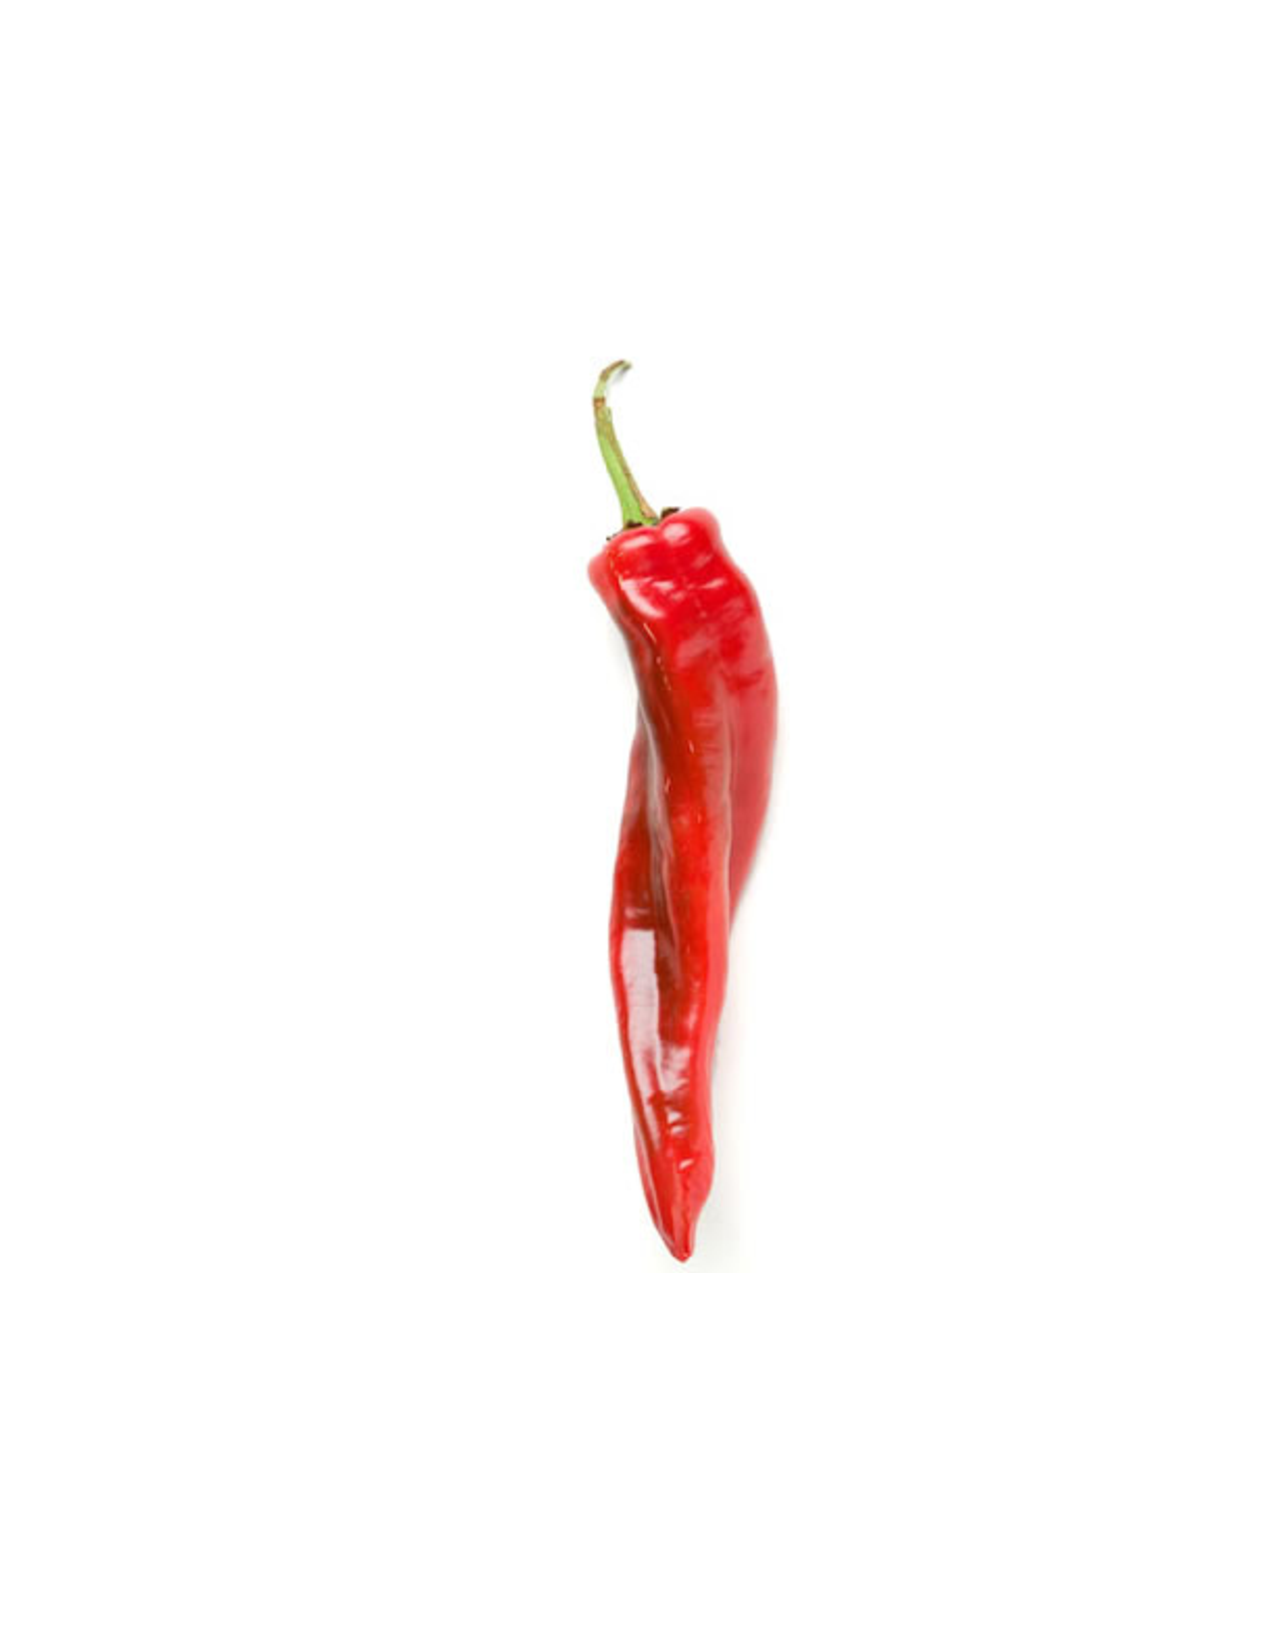
\includegraphics{figures/chili.pdf}}}
\newcommand{\chchili}{{\chili\chili}}
\newcommand{\chchchili}{{\chchili\chili}}

% The units package provides nice, non-stacked fractions and better spacing
% for units.
\usepackage{units}

% The fancyvrb package lets us customize the formatting of verbatim
% environments.  We use a slightly smaller font.
\usepackage{fancyvrb}
\fvset{fontsize=\normalsize}

% Small sections of multiple columns
\usepackage{multicol}

\hypersetup{
urlcolor=blue,
colorlinks=true
}
\usepackage[noline, procnumbered, linesnumberedhidden, boxed]{algorithm2e}

\newcommand{\openepigraph}[2]{ % This block sets up a command for printing an epigraph with 2 arguments - the quote and the author
\begin{fullwidth}
\sffamily\large
\begin{doublespace}
\noindent\allcaps{#1}\\ % The quote
\noindent\allcaps{#2} % The author
\end{doublespace}
\end{fullwidth}
}

\newcommand{\figref}[1]{Figure~\ref{#1}}
\renewcommand{\thefigure}{\arabic{figure}}

\newenvironment{callout}[1]{
\[
  \left[
      \begin{tabular}{@{\quad}m{.05\textwidth}@{\qquad}m{.75\textwidth}@{\quad}}
        \scalebox{1.5}{#1} & 
          \raggedright%
}
{
      \end{tabular}
    \right]
\]
}

\newcommand{\blankpage}{\newpage\hbox{}\thispagestyle{empty}\newpage} % Command to insert a blank page

\usepackage{makeidx} % Used to generate the index
\makeindex % Generate the index which is printed at the end of the document

\renewcommand{\maketitlepage}[0]{%
  \cleardoublepage%
  {%
  \sffamily%
  \begin{fullwidth}%
  ~
  \vspace{11.5pc}%
  \fontsize{36}{40}\selectfont\par\noindent\textcolor{darkgray}{\allcaps{\thanklesstitle}}%
  
\scalebox{.2}{
\includegraphics{figures/msan-logo}}
  \vspace{11.5pc}%
  \fontsize{12}{18}\selectfont\par\indent\textcolor{darkgray}{\allcaps{\thanklessauthor}\\
\indent{\tt parrt@cs.usfca.edu}\\
\href{http://parrt.cs.usfca.edu}{http://parrt.cs.usfca.edu}}%
  \vspace{11.5pc}%
  \fontsize{14}{16}\selectfont\par\noindent\allcaps{\thanklesspublisher}%
  \end{fullwidth}%
  }
  \thispagestyle{empty}%
  \clearpage%
}

\titlecontents{part}% FIXME
    [0em] % distance from left margin
    {\vspace{1.5\baselineskip}\begin{fullwidth}\LARGE\rmfamily\itshape} % above (global formatting of entry)
    {\contentslabel{2em}} % before w/label (label = ``II'')
    {} % before w/o label
    {\rmfamily\upshape\qquad\thecontentspage} % filler + page (leaders and page num)
    [\end{fullwidth}] % after

  \titlecontents{chapter}%
    [0em] % distance from left margin
    {\vspace{1.5\baselineskip}\begin{fullwidth}\Large\rmfamily\itshape} % above (global formatting of entry)
    {\hspace*{0em}\contentslabel{2em}} % before w/label (label = ``2'')
    {\hspace*{4em}} % before w/o label
    {\rmfamily\upshape\qquad\thecontentspage} % filler + page (leaders and page num)
    [\end{fullwidth}] % after

\titlespacing*{\chapter}{0pt}{0pt}{30pt}
\titlespacing*{\section}{0pt}{3.5ex plus 1ex minus .2ex}{2.3ex plus .2ex}
\titlespacing*{\subsection}{0pt}{3.25ex plus 1ex minus .2ex}{1.5ex plus.2ex}

\begin{document}

\chapter{Git on it}

{\em\small For our purposes in MSAN, we're going to ignore most of the nontrivial capabilities that programmers use routinely, such as branching and merging. Git is extremely  complicated and would not be my first choice if it weren't for the excellent {\tt github.com}.}

\section{Introduction to revision control}

{\em Revision control} is a mechanism to track all changes to a set of files, which we typically associate with the project. The file set is called a {\em repository} and at any given time, my computer has lots and lots of these repositories. 

A {\tt git} repository instance is just a directory on your disk that also happens to have a {\tt .git} (hidden) directory, which is effectively a complete database of everything that's happened to the repository since it was created with {\tt git init} (or you {\tt clone}'d it from somewhere). 

If you want to throw out the repository, just remove the entire subtree from your disk. There is no central server to notify. Every repository instance is a complete copy so you could have, for example, 10 versions of the repository cloned from an original sitting on the same disk.

After you create a repository, you can create all sorts of files in the local directories managed by git, but git ignores them until you {\tt add} them. {\tt add} is basically notifying the repository that it should care about the file. When you add files or modify files already known to git, they are in the so-called staging area (this used to be called the index). You can have whatever other files you want laying around, such as development environment preference files. Git will simply ignore them unless you {\tt add} them. This is different than other revision control systems that insist upon knowing about and managing everything under a particular subtree. I like this feature.

\subsection{Does a solo programmer need revision control?}

If you are working solo, from a single machine, and you have a regular backup mechanism in your development environment or from the operating system like Time Machine (OS X), you can get away without a formal revision system.

There are lots of important operations that can be faked without a revision system.  For example, it's a good idea to keep track of versions of the software that work or other milestones. In the old days, people would make a copy of their project directory corresponding to important milestones like "Added feature X and it seems to work." You can do comparisons using a diff tool in between directories.

Whether your IDE does it or a revision control system does it, I find it very important to look back at recent changes to see what changes have introduced a bug.  Sometimes I decide to abandon a small piece of what's going on and flip a file back to an old version.

A good example of use of a repository is the repository for this course, which is stored at {\tt github.com} as well as my desktop computer (and laptop, and home machine, ...):

\href{https://github.com/parrt/msan501}{\textcolor{blue}{https://github.com/parrt/msan501}}

\noindent It contains all the changes that I've made since I started teaching this course.

These days, revision control systems are meant to be used among multiple computers and multiple developers, but they are still useful even on a single machine.

\subsection{Solo programmer, sharing across machines}

In order to work on that software from your home machine and a laptop for example, you have to make copies. That introduces the possibility that you will overwrite the good version of your software. Or, you will forget that you had made changes on your laptop but have now made a bunch of changes on your desktop.  You have changes on two different computers. Resolving things can be tricky and error-prone.

Enter a remote server such as {\tt github.com}. It acts like a big disk that holds lots of different repositories per user. I normally create a repository at the website, then grab the repository URL, and {\tt clone} it onto my local disk of any machine that needs to share the code. The process of sharing changes looks like this:

\begin{enumerate}
\item Laptop: pull any changes from the github repository
\item Laptop: Make changes
\item Laptop: Push changes to github server
\item Desktop: pull changes from the github repository (stuff you just changed)
\item Desktop: Make changes
\item Desktop: Push changes to github server
\end{enumerate}

The github repository acts as a central repository, which is a change of perspective. Normally we think of our computer is having the primary copy.

As a side benefit, pushing your repository to a remote server gives you a backup automatically.

\subsection{Multiple programmers}

When you add another person to a project, people end up mailing code around but it's difficult to perform a merge. My experience watching students do this reveals that two versions of the software always appear. Both students shout that their version is better and that the other version should be abandoned.

In my experience, no matter how you try to fake multiple states of the source code and share, merging changes to work on the same code base is a nightmare.

Once in a while I go back and I look at the history of changes. Sometimes I want to know who screwed this up or I want to see the sequence of changes that I made or that were made by somebody else.

Every single commercial developer I know uses revision control at work. Every company you will encounter uses it. For that reason alone, you need to learn revision control to be functional in a commercial setting.

\section{Cloning an existing repository}

{\em I've deleted the section. Please see the discussion in the images project related to} {\tt git}.

\section{PyCharm + git = no problem}

{\em I've deleted the section. Please see the ``Adding files to your repo'' discussion in the images project}.

\section{Git from the command line}

{\bf Adding to repo}. To add files, just create them and do a {\tt commit}:

\begin{lstlisting}[style=BashInputStyle]
$ cd ~/myrepo
$ mkdir junk
$ cd junk
... create t.py ...
$ git add t.py
$ git commit -a -m 'initial add'
\end{lstlisting}

\noindent You can also create files and subdirectories:

\begin{lstlisting}[style=BashInputStyle]
$ cd ~/myrepo
$ mkdir junk
$ cd junk
... create t2.py ...
$ git add t2.py
$ git commit -a -m 'add 2nd file'
\end{lstlisting}

\noindent {\bf Make changes}. You can make changes and do another commit. Make sure use the {\tt -a} option on the {\tt git commit}. 

\noindent {\bf Deleting files}. Deleting a file is also considered a change but you can also use {\tt git rm} {\em filename}.

\noindent {\bf Checking differences with repo}. If you make a change and want to know how it's different from the current repository version, just use diff:

\begin{lstlisting}[style=BashInputStyle]
$ ... tweak t.py ...
$ git diff t.py
...
\end{lstlisting}

\noindent {\bf Reverting}. If you screw up and want to toss out everything from the last commit, do a reset and make sure you use the hard option:

\begin{lstlisting}[style=BashInputStyle]
$ ... tweak whatever you want ...
$ git reset --hard HEAD
\end{lstlisting}

\noindent which throws out all changes since the last commit. If all you want to do is revert uncommitted changes to a single file, you can run this:

\begin{lstlisting}[style=BashInputStyle]
$ git checkout -- filename
\end{lstlisting}

I think they call that funny dash-dash option ``sparse mode.'' (Git is the machine code of revision systems. blech.)

\noindent {\bf Correcting commit message}. One of the other things I often have to do is to fix the commit message that I just wrote in a commit command.

\begin{lstlisting}[style=BashInputStyle]
$ git commit --amend -m "I really wanted to say this instead"
\end{lstlisting}

\noindent {\bf Adding file you forgot to commit}. If you forgot to add one of the files and you wanted in a previous commit, you can also use amend. Just add the file and use amend:

\begin{lstlisting}[style=BashInputStyle]
$ git add t2.py
$ git commit --amend --no-edit
\end{lstlisting}

{\bf Checking working dir and staging area vs repo.} Finally, if you want to figure out what changes you have made such as adding, deleting, or editing files, you can run:

\begin{lstlisting}[style=BashInputStyle]
$ git status
On branch master
Your branch is up-to-date with 'origin/master'.

Untracked files:
  (use "git add <file>..." to include in what will be committed)

    t3.py

nothing added to commit but untracked files present (use "git add" to track)
\end{lstlisting}

\section{Don't fear {\tt commit}ment}

Every time you {\em commit} a change (file edit, file add, file delete, ...) to the repository, the revision control system tracks a patch called the {\em diff} that indicates essentially how to edit the first file version in order to arrive at the current file version. Storing just the differences is very space efficient and  lets the revision control system apply the same set of changes to a file on a different computer to keep them both in sync.  

Having a complete list of changes is extremely useful. For example, here is a chunk taken out of the middle of my commits on the ANTLR repository as shown by SourceTree:

\scalebox{.85}{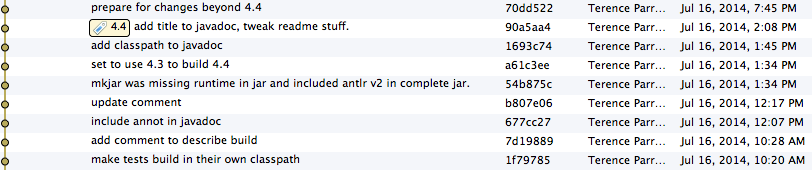
\includegraphics{figures/commits.png}} 

That should look very much like Time Machine on OS X to you. You can go back and look at changes made to the repository for any commit.

You will also notice that I have tagged a particular commit as 4.4 with the tag command. This makes it easy for me to flip the repository back to a specific commit with a name rather than one of those funky commit checksums.

You should commit only logical chunks like feature additions, bug fixes, or comment updates across the project, etc.

Commit messages are important. Do not use meaningless messages, as I see students sometimes do:

\begin{alltt}
Add t.py
Alter t.py
Change t.py
...
\end{alltt}

I have even seen git commit messages: {\tt one}, {\tt two}, {\tt three}. Nothing spells laziness or academic dishonesty than that.

In rare cases, when I'm working alone, I sometimes use a private repository as a means of sharing files across multiple computers like dropbox. In this case, my commits are just to take a snapshot to pull it down on another machine. The commit message doesn't matter (though I might still look back through the changes at some point). When doing this for a real project, it's best to use stash per the next section.

\section{With a remote server like github}

When you're working by yourself (and without branches), a remote server acts like a central server that you can push and pull from. For example, I push from my work machine and pull to my home machine or my laptop. And then reverse the process with changes I make at home over the weekend.

For example, once I have commit all of my changes that work and I'm ready to go home, I push to the origin:

\begin{lstlisting}[style=BashInputStyle]
$ git push origin master
\end{lstlisting}

\noindent From home, I do:

\begin{lstlisting}[style=BashInputStyle]
$ git pull origin master
\end{lstlisting}

\noindent The origin is the alias for the original server we cloned from and master is our master branch, which we can ignore until we look at branches.

To look at the remote system alias(es), we use:

\begin{lstlisting}[style=BashInputStyle]
$ git remote -v
origin  git@github.com:parrt/myrepo.git (fetch)
origin  git@github.com:parrt/myrepo.git (push)
\end{lstlisting}

\end{document}


\part{Python Programming and Data Structures}

\chapter{Image Processing}

\setcounter{problem}{1}

\noindent The goal of this chapter is to exercise your understanding of all of the major components in Python: {\bf assignments, expressions, if and loop statements, functions, lists, and libraries}. To make things interesting, we will perform some cool image processing tasks: {\bf flipping horizontally, blurring, removing salt-and-pepper image noise, finding edges within images, and image sharpening}.  For example, \figref{sharpbonkers} demonstrates image sharpening.

\begin{marginfigure}
\begin{center}
\scalebox{.45}{
\includegraphics{figures/bonkers-bw-zoom.png}}
\scalebox{.45}{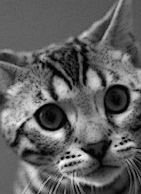
\includegraphics{figures/bonkers-sharp-zoom.png}}
\end{center}
\caption{Bonkers the cat sharpened using {\tt sharpen.py}.}
\label{sharpbonkers}
\end{marginfigure}

\section{Installing Pillow}

For image processing, we'll use Pillow, so please follow the instructions carefully to install \href{http://pillow.readthedocs.org/en/latest/installation.html}{\textcolor{blue}{Pillow, a fork of PIL}}.

\subsection{Install stuff on a mac}

First make sure {\tt brew} is installed; try this from Terminal app:

\begin{lstlisting}[style=BashInputStyle]
$ brew
\end{lstlisting}

\noindent If not there, go here: {\tt http://brew.sh} and it'll say to install do this:

\begin{lstlisting}[style=BashInputStyle]
$ ruby -e "$(curl -fsSL https://raw.githubusercontent.com/Homebrew/install/master/install)"
\end{lstlisting}

\noindent then

\begin{lstlisting}[style=BashInputStyle]
$ brew install python
\end{lstlisting}

\noindent That should give you pip as well.  Ignore warning about having 2 pythons installed.  Make sure python is using the brew version of python. All brew stuff is in {\tt /usr/local/Cellar/*} so you should see:

\begin{lstlisting}[style=BashInputStyle]
$ which python
/usr/local/bin/python
$ ls -l `which python`
lrwxr-xr-x  1 parrt  admin  33 Jul  5 12:19 /usr/local/bin/python@ -> ../Cellar/python/2.7.9/bin/python
\end{lstlisting}

\noindent Now, install all of the software you need before installing Pillow:

\begin{lstlisting}[style=BashInputStyle]
$ brew install libtiff libjpeg webp little-cms2
\end{lstlisting}

\noindent then

\begin{lstlisting}[style=BashInputStyle]
$ pip install Pillow
\end{lstlisting}

\noindent If you get an error that ends with:

\begin{alltt}
    ...
    ImportError: cannot import name HTTPSHandler
\end{alltt}

\noindent then try reinstalling python:

\begin{lstlisting}[style=BashInputStyle]
$ brew reinstall python
\end{lstlisting}
\noindent Test it:

\begin{lstlisting}[style=BashInputStyle]
$ python
Python 2.7.9 (default, Jul  5 2015, 12:18:15) 
[GCC 4.2.1 Compatible Apple LLVM 6.0 (clang-600.0.57)] on darwin
Type "help", "copyright", "credits" or "license" for more information.
>>> import PIL
>>>
\end{lstlisting}

\noindent there should be no error when you type {\tt import PIL}

\section{Getting started}

To get started, review how to access the \href{http://stackoverflow.com/questions/4117530/sys-argv1-meaning-in-script}{\textcolor{blue}{command-line arguments}} that every program running on a computer can accept. Here is a small program, {\tt view.py}, that accepts a filename as a command-line argument.

\begin{pyverbatim}
import sys
from PIL import Image
if len(sys.argv) != 2:
	print "$ python view.py imagefilename"
	sys.exit(1)
filename = sys.argv[1] # get the argument passed to us by operating system
img = Image.open(filename) # load file specified on the command line
img = img.convert("L") # grayscale
img.show()
\end{pyverbatim}

To run this program, launch a terminal on Mac or Linux. Then, move to the directory that contains {\tt view.py} that you saved/typed-in using terminal command {\tt cd} (change directory).  For example, if you are using directory {\tt msan501/images} under your home directory for this project, then type this for Mac:

\begin{lstlisting}[style=BashInputStyle]
cd /Users/YOURID/msan501/images
\end{lstlisting}

\noindent and this for Linux:

\begin{lstlisting}[style=BashInputStyle]
cd /home/YOURID/msan501/images
\end{lstlisting}

You can get a bunch of sample images that I use for these notes from github:

{\tt https://github.com/parrt/msan501/tree/master/labs/figures}

\noindent but of course you can play around with whatever images you want.\sidenote{Remember, however, that all images used in this class and those stored on University equipment must be ``safe for work.'' Keep it G-rated please, with no offensive images popping up on your laptops or machines during lab etc.}

\noindent Now, we can execute our {\tt view.py} script and pass it an argument of {\tt obama.png}:

\begin{lstlisting}[style=BashInputStyle]
$ python view.py obama.png
\end{lstlisting}

If you are using PyCharm, then you need to use the ``{\tt\small Edit configuration}'' dialog under the {\tt Run} menu.  All file names that we specify in the script parameters area, or from the command line, are relative to the {\em current working directory}. That is why we used {\tt cd} to change our working directory in the example above. For convenience, let's keep all of images and scripts in the same directory. For our purposes, let's assume that the directory is always {\tt\small /Users/YOURID/msan501/images} (Mac) or {\tt\small /home/YOURID/msan501/images} (Linux).

\scalebox{1}{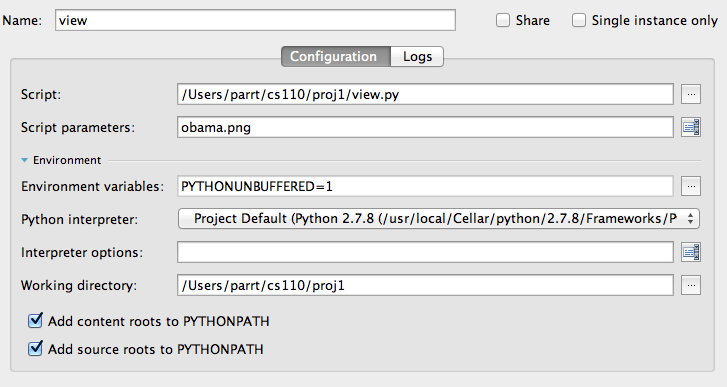
\includegraphics{figures/edit-config.png}}

The ``Script parameters'' text field is where you provide the ``command-line arguments,'' despite the fact we are not actually using a command-line. That is why PyCharm calls it script parameters instead of command-line parameters.

\section{Task 1. Flipping an image horizontally}

As a first task, you must create a script called {\tt flip.py} that shows the image provided as a program (command-line) argument in its original form and then flipped horizontally.  For example, \figref{flipped} shows the result of running script {\tt flip.py} on image {\tt eye.png}.

\begin{marginfigure}
\begin{center}
\scalebox{.49}{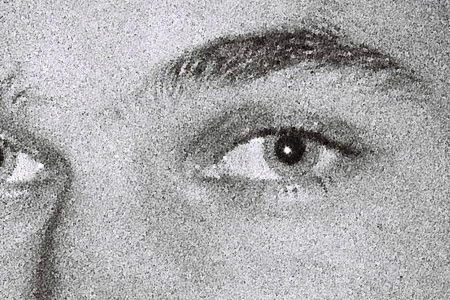
\includegraphics{figures/eye.png}} \scalebox{.49}{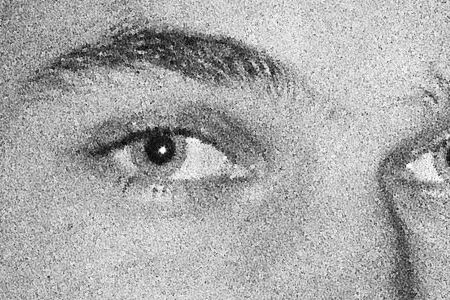
\includegraphics{figures/eye-flip.png}}
\end{center}
\caption{Flipping an image horizontally; the original is on the left.}
\label{flipped}
\end{marginfigure}

\subsection{Boilerplate code}

Here's the boilerplate or ``skeleton'' code (already in repo as {\tt images/flip.py}) that we already know how to do but with a hole where you need to define a function called {\tt flip} and a hole where you need to call that function to perform the flipping:

\begin{pyverbatim}
import sys
from PIL import Image

# define your flip function here
...
if len(sys.argv)<=1:
	print "missing image filename"
	sys.exit(1)
filename = sys.argv[1]
img = Image.open(filename)
img = img.convert("L")
img.show()

# call your flip function here
...
img.show()
\end{pyverbatim}

If you are using PyCharm, your project file list area should look like the list in \figref{fliplist}. It assumes that you have downloaded two image files as well.

\begin{marginfigure}
\begin{center}
\scalebox{.8}{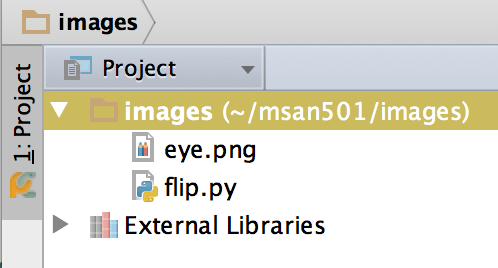
\includegraphics{figures/flip-proj-browser.png}}
\end{center}
\caption{Project file list after building the flip task}
\label{fliplist}
\end{marginfigure}

The files are already in the repository because I did the following:

\begin{lstlisting}[style=BashInputStyle]
$ cd ~/msan501/images
$ git add eye.png
$ git add flip.py
$ git commit -a -m 'add eye flip boilerplate code and image'
[master adcf1df] add eye flip boilerplate code and image
 2 files changed, 16 insertions(+)
 create mode 100644 images/eye.png
 create mode 100644 images/flip.py
$ git push origin master
Counting objects: 5, done.
Delta compression using up to 8 threads.
Compressing objects: 100% (5/5), done.
Writing objects: 100% (5/5), 238.35 KiB | 0 bytes/s, done.
Total 5 (delta 0), reused 0 (delta 0)
To git@github.com:parrt/msan501-starterkit.git
   b5820e1..adcf1df  master -> master
\end{lstlisting}

\subsection{Three new Pillow pieces}

To write your {\tt flip} function, you will need three basic pieces:

\begin{itemize}
\item {\tt img.size} returns a tuple containing the width and height of image {\tt img} so you can write code like this:
\begin{pyverbatim}
width, height = img.size
\end{pyverbatim}
You'll need the width and height to iterate over the pixels of the image.

\item {\tt img.copy()} duplicates image {\tt img}.  For our {\tt flip} function, it would be hard to modify the image in place because we would be overwriting pixels we would need to flip later. It's easier to create a copy of the image in flipped position. You can write code like this:\\
{\tt imgdup = img.copy()}

\item {\tt img.load()} is yet another weird name from PIL that actually returns an object that looks like a two-dimensional matrix. We have previously seen two-dimensional lists, which are really like lists of lists such as {\tt m = [[1,2], [3, 4]]} or reformatted to look like the matrix:
\begin{pyverbatim}
m = [[1, 2],
     [3, 4]]
\end{pyverbatim}
To get element {\tt 3}, we would use list index expression {\tt m[1][0]} because we want the list at index 1, {\tt m[1]}, and then element 0 within that list. The two-dimensional object returned by {\tt load()} uses similar notation. If we ask for the ``matrix'' with:
\begin{pyverbatim}
m = img.load()
\end{pyverbatim}
then we would use notation {\tt m[x,y]} to get the pixel at position ({\tt x}, {\tt y}).
\end{itemize}

You will use these functions for the remaining tasks so keep them in mind.

\subsection{Iterating over the image matrix}

{\bf Define function} {\tt flip} using the familiar function definition syntax and have it take a parameter called {\tt img}, which will be the image we want to flip. The goal is to create a copy of this image, flip it, and return a copy so that we do not alter the incoming original image. To create {\tt flip}, write code that implements the following steps.

\begin{enumerate}
\item Use {\tt size} to define local variables {\tt width} and {\tt height}
\item Use {\tt copy()} to make a copy of the incoming image {\tt img} and save it in a local variable
\item Use {\tt load()} to get the two-dimensional pixel matrix out of the incoming image and the copy of the image. Store these results in two new local variables.
\item To walk over the two-dimensional image, we've learned we need every combination of {\tt x} and {\tt y}. That means we need a nested {\tt for} loop. Create a nested for loop that iterates over all {\tt x} and all {\tt y} values within the {\tt width} and {\tt height} of the image.
\item Within the inner loop, set pixels in the image copy to the appropriate pixel copied from the original image
\item At the end of the function, return the flipped image
\end{enumerate}

The only remaining issue is determining which pixel from the original image to copy into the ({\tt x}, {\tt y}) position in the image copy. The {\tt y} index will be the same since we are flipping horizontally. The {\tt x} index in the flipped image is index {\tt width-x-1} from the original image. Trying out a few sample indexes shows that this works well. For example, a flipped image with {\tt width=10} has its pixel at {\tt x=0} pulled from index {\tt x=10-0-1=9} in the original image. That's great, because it takes the image from all in the right in the original and copies it to the far left of the copy. Checking the opposite extreme, {\tt x=9} in the flipped image should be {\tt x=10-9-1=0} from the original image.

\subsection{Running your flip script}

{\bf To run the script from the command line}, make sure you are in the {\tt msan501/images} directory containing your scripts and images then do:

\begin{lstlisting}[style=BashInputStyle]
$ cd msan501/images
$ python flip.py eye.png
\end{lstlisting}

{\bf From PyCharm}, I right-click and then select ``Run.'' It will do nothing but print ``{\tt missing image filename}'' because we have not given it a parameter yet, but we need to do this so that PyCharm creates a run configuration. Now, use the edit configuration dialog to specify {\tt eye.png} as a parameter or any other image. ({\em Remember that the filename must refer to a file in the current working directory or must be fully qualified.}) Click ``Run'' now and it should bring out the two images.

\scalebox{.82}{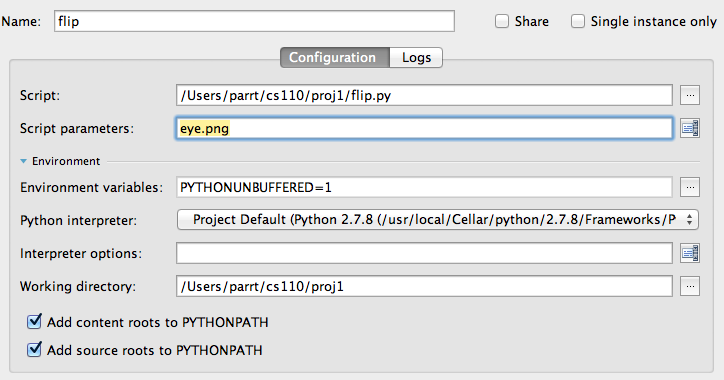
\includegraphics{figures/flip-config.png}}

\subsection{What to do when the program doesn't work}

If you have problems, follow these steps:

\begin{enumerate}
\item Don't Panic! Relax and realize that you will solve this problem, even if it takes a little bit of messing around. Banging your head against the computer is part of your job. Remember that the computer is doing precisely what you tell it to do. There is no mystery.
\item  Determine precisely what is going on. Did you get an error message from Python?  Is it a syntax error? If so, review the syntax of all your statements and expressions. PyCharm is your friend here and should highlight erroneous things with a red squiggly underline. If you got an error message that has what we call a stack trace, a number of things could be wrong. For example, if I misspell {\tt show()} as {\tt shower()}, I get the following message:
\begin{alltt}\small
Traceback (most recent call last):
  File "/Users/parrt/msan501/images/flip.py", line 26, in <module>
    img.shower()
  File "/usr/local/lib/python2.7/site-packages/PIL/Image.py", line 605, in __getattr__
    raise AttributeError(name)
AttributeError: shower
\end{alltt}
In PyCharm, the ``{\tt /Users/parrt/msan501/images/flip.py}'' part of the trace will be a blue link that you can click on. It will take you to the exact location in your script where there is a problem. Look for anything that refers to that file.
\item If it does not look like it some simple misspelling, you might get lucky and find something in Google if you cut-and-paste that error message.
\item If your script shows the original image but not the flipped image, then you likely have a problem with your {\tt flip} function.
\item If your program is at least running and doing something, then insert print statements to figure out what the variables are and how far into the program you get before a craps out. That often tells you what the problem is.
\item Try using the debugger to step through your program in PyCharm. Set a breakpoint on for example the line {\tt filename = sys.argv[1]} by clicking in the gutter to the left of that line.  A red dot should appear, indicating there is a breakpoint there. Then click the little bug icon instead of the green triangle (which is run button). That will start execution and then stop at that line. You can look at all of the variables at that point. Then you can step forward line by line. Read how to use the debugger online.
\item  Definitely try to solve the problem yourself, but don't waste too much time. I can typically help you out quickly so you can move forward.
\end{enumerate}

\begin{callout}{\bcplume}
{\bf Deliverables}. Make sure that {\tt images/flip.py} is correctly committed to your repository and pushed to github. 
\end{callout}

\section{Task 2. Blurring}

In this task, we want to blur an image by removing detail as shown in \figref{blur}. We will do this by creating a new image whose pixels are the average of the surrounding pixels for which we will use a 3x3 region as shown in \figref{region}. The pixel in the center of the region is the region to compute as we slide the region around an image. In other words, {\tt pixel[x,y]} is the sum of {\tt pixel[x,y]} and all surrounding pixels divided by 9, the total number of pixels.

\begin{marginfigure}
\begin{center}
\scalebox{.87}{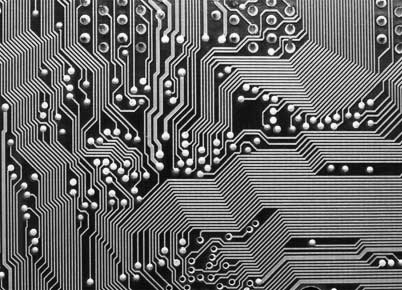
\includegraphics{figures/pcb.png}}\\
\scalebox{.87}{
\includegraphics{figures/pcb-blur.png}}
\end{center}
\captionof{figure}{Blurring of a circuit board; the original is on top.}
\label{blur}
\end{marginfigure}

To implement this, start with the boilerplate from the previous section, which you should put into script {\tt blur.py}. The only difference is that you must call soon-to-be-created function {\tt blur} not {\tt flip} as you had before. Now, let's start at the courses level of functionality and realize that we have to walk over every pixel in the image. (This is called {\em top-down design}.) 

\subsection{Blurring function}

{\bf Define function} {\tt blur} to take an {\tt img} parameter, just like the {\tt flip} function in the previous task.  In a manner very similar to {\tt flip}, write code in {\tt blur} to accomplish these steps:

\begin{enumerate}

\item Define local variables {\tt width} and {\tt height}.
\item Make a copy of the incoming image {\tt img} and save it in a local variable.
\item Get the two-dimensional pixel matrix out of the image copy. Store it in a new local variable called {\tt pixels}.
\item Create a nested for loop that iterates over all {\tt x} and all {\tt y} values within the {\tt width} and {\tt height} of the image.
\item Within the inner loop:
\begin{enumerate}
\item Call to-be-created function {\tt region3x3} with arguments {\tt img}, {\tt x}, and {\tt y} in store into local variable {\tt r}.
\item Set {\tt pixels[x,y]} in the image copy to the result of calling to-be-created function {\tt avg} with an argument of {\tt r}.
\end{enumerate}
\item At the end of the function, return the flipped image.
\end{enumerate} 

Following the top-down design strategy, let's {\bf define function} {\tt avg} since it's the easiest. Define {\tt avg} to take an argument called {\tt data} or another of your choice. This will be the list of 9 pixels returned by function {\tt region3x3}. The average of a set of numbers is their total divided by how many numbers there are. Python provides two useful functions here: {\tt sum(data)} and {\tt len(data)}.  (Naturally, {\tt sum} simply walks the list and accumulates values using a pattern we are familiar with.)

\subsection{Image regions}

Now we need to {\bf define function} {\tt region3x3}.  Have it take three parameters as described above. This function creates and {\bf return a list of nine pixels}. The list includes the center pixel at {\tt x}, {\tt y} and the 8 adjacent pixels at N, S, E, W, ... as shown in \figref{region}. Create a series of assignments that look like this:

\begin{marginfigure}
\begin{center}
\scalebox{1}{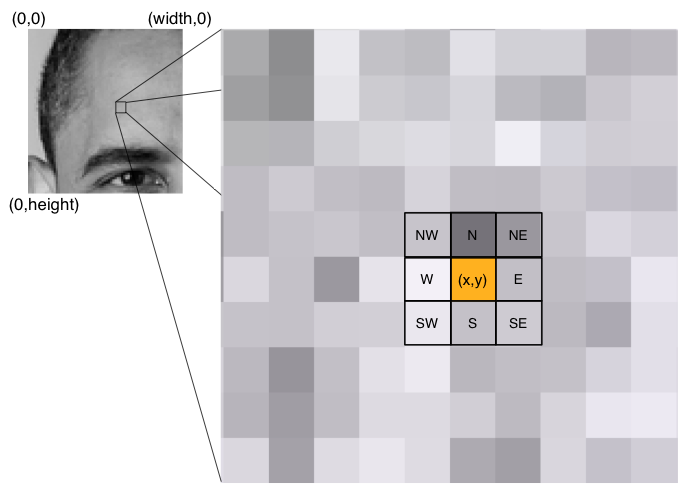
\includegraphics{figures/region.png}}
\end{center}
\captionof{figure}{Hyper-zoom of Obama's forehead showing 3x3 region.}
\label{region}
\end{marginfigure}

\begin{pyverbatim}
me = getpixel(img, x, y)
N = getpixel(img, x, y - 1)
...
\end{pyverbatim}

\noindent where function {\tt getpixel(img, x, y)} gets the pixel at {\tt x}, {\tt y} in image {\tt img}.  We can't use the more readable expression {\tt pixels[x,y]} in this case, as we'll see in a second. Collect all those pixel values into a list using {\tt [a,b,c,...]} list literal notation and return it. Make sure that this list is a list of integers and exactly 9 elements long and that you keep in mind the order in which you add these pixels to the list. Any function that we create to operate on a region naturally needs to know the order so we can properly extract pixels from the list. For example, my implementation always puts the pixel at {\tt x} and {\tt y} first, then North, etc...

\subsection{Safely examining region pixels}

We need to {\tt define a function} {\tt getpixel} instead of directly accessing pixels because some of the pixels in our 3x3 region will be outside of the image as we shift the region around. For example, when we start out at {\tt x=0}, {\tt y=0}, 5 of the pixels will be out of range, as shown in \figref{outofrange}.  Accessing {\tt pixels[-1,-1]} will trigger:

\begin{marginfigure}
\begin{center}
\scalebox{.85}{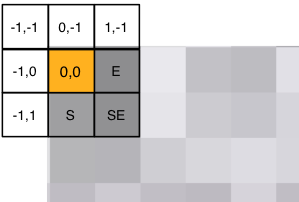
\includegraphics{figures/region-edge.png}}
\end{center}
\captionof{figure}{Our 3x3 region has pixels outside of the image boundaries as we slide it around the image along the edges.}
\label{outofrange}
\end{marginfigure}

{\tt IndexError: image index out of range}

\noindent and stop the program. To avoid this error and provide a suitable definition for the ill-defined pixels on the edges, we will use a function that ensures all indices are within range.

{\bf Define function} {\tt getpixel} with the appropriate parameters. Its functionality is as follows:
\begin{enumerate}
\item Get the width and height into local variables.
\item If the {\tt x} value is less than 0, set it to 0.
\item If the {\tt x} value is greater than or equal to the width, set it to the width minus 1 (the last  valid pixel on the far right).
\item If the {\tt y} value is less than 0, set it to 0.
\item If the {\tt y} value is greater than or equal to the height, set it to the  height minus 1 (the last felt pixel on the bottom).
\item Return the pixel at {\tt x}, {\tt y}. You will need to use the {\tt img.load()} function again to get the 2D {\tt pixels} matrix as you did in function {\tt blur}. Make sure you returning pixel and not the coordinates of the pixel from {\tt getpixel}.
\end{enumerate}

\subsection{Testing your blur code}

That is a lot of code to enter and so more than likely it won't work the first time.\sidenote{It never does, dang it!} That means we should test the pieces. It's generally a good idea to do top-down design but {\em bottom-up testing}. In other words, let's test the simple low-level functions first and make sure that works before testing the functions that call those functions and so on until we reach the outermost script. 

With that in mind, lets test {\tt avg} by passing it a fixed list of numbers to see if we get the right number. Add this to your script before it does any of the file loading stuff:

\begin{pyverbatim}
print avg([1,2,3,4,5])
\end{pyverbatim}

\noindent Then run {\tt blur.py} with any old image; the {\tt apple.png} file is a good one because it's small:

\begin{lstlisting}[style=BashInputStyle]
$ python blur.py apple.png
3
$ 
\end{lstlisting}

\noindent If it does not print $(1+2+3+4+5)/5 = 3$, then you know you have a problem in {\tt avg}.

Now test {\tt getpixel}. You will have to insert some code after loading and converting the image to grayscale because {\tt getpixel} takes an image parameter:

\begin{pyverbatim}
img = Image.open(filename)
img = img.convert("L")
print getpixel(img, 0, 0)
print getpixel(img, 0, 1)
print getpixel(img, 10, 20)
\end{pyverbatim}

\noindent  That should print: 96, 96, and 255. The upper left corner is gray and pixel 10, 20 is somewhere in the middle of the white Apple logo. If you don't get those numbers, then you have a problem with {\tt getpixel}. Worse, if you don't get simple numbers, then you really have a problem with {\tt getpixel}.

Before getting to {\tt blur}, we should also {\bf test} {\tt region3x3} to ensure it gets the proper region surrounding a pixel. Replace those {\tt getpixel} calls in the {\tt print} {\tt getpixel} statements with calls to {\tt region3x3}. Use the {\tt x}, {\tt y} of the upper left-hand corner and somewhere near the upper left of the white section of the logo such as:

\begin{pyverbatim}
print region3x3(img, 0, 0)
print region3x3(img, 7, 12)
\end{pyverbatim}

\noindent That checks whether we get an out of range error at the margins and that we get the correct region from somewhere in the middle. Running the script should give you the following numbers:

\begin{lstlisting}[style=BashInputStyle]
$ python blur.py apple.png
[96, 96, 96, 96, 96, 96, 96, 96, 96]
[255, 176, 255, 255, 215, 96, 245, 255, 255]
$ 
\end{lstlisting}

\noindent That assumes order: current pixel, N, S, E, W, NW, NE, SE, SW.

When you have verified that all of these functions work, it's time to check function {\tt blur} itself. Try the printed circuit board image:

\begin{lstlisting}[style=BashInputStyle]
$ python blur.py pcb.png 
\end{lstlisting}

\noindent That should pop up the original circuit board and the blurred version. It might take 10 seconds or more to compute and display the blurred image, depending on how fast your computer is.

\begin{callout}{\bctakecare}
Make sure to remove all of your debugging code before submitting your scripts. Submitting a project with a bunch of random debugging output is considered sloppy, like submitting an English paper with a bunch of handwritten edits.
\end{callout}

\begin{callout}{\bcplume}
{\bf Deliverables}. Make sure that {\tt images/blur.py} is correctly committed to your repository and pushed to github.
\end{callout}

\section{Task 3. Removing noise}

For our next task, we are going to de-noise (remove noise) from an image as shown in \figref{obama}. It does a shockingly good job considering the simplicity of our approach. To blur, we used the average of all pixels in the region. To denoise, we will use the \href{http://en.wikipedia.org/wiki/Median}{\textcolor{blue}{median}}, which is just the middle value in a list of ordered numbers.

Believe it or not, we can implement the noise by copying {\tt blur.py} into a new script called {\tt denoise.py} and then changing a few lines.  We also have to remove the  no-longer-used {\tt avg} function and replace it with a {\tt denoise} function.  Of course, instead of calling {\tt blur}, we'll call function {\tt denoise} with the usual {\tt img} argument. The only difference between {\tt denoise} and {\tt blur} is that you will set the pixel to the {\tt median} not {\tt avg}.  Hint: you need to tweak one statement in the inner loop that moves over all pixel values.

{\bf Now define function} {\tt median} that, like {\tt avg}, takes a list of 9 numbers called {\tt data}. Sort the list using Python's {\tt sorted} function that takes a list and returns a sorted version of that list. Then compute the index of the middle list element, which is just the length of the list divided by two. If the length is even, dividing by 2 (not 2.0) will round it down to the nearest index. Once you have this index, return the element at that index.

\begin{marginfigure}
\begin{center}
(a) \scalebox{.5}{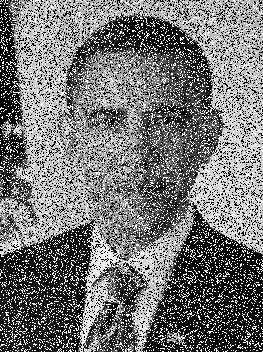
\includegraphics{figures/guesswho.png}}\\
(b) \scalebox{.5}{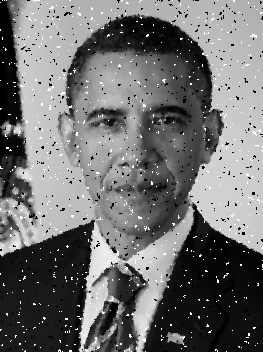
\includegraphics{figures/guesswho-denoise.png}}\\
(c) \scalebox{.5}{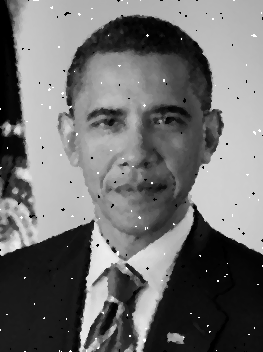
\includegraphics{figures/guesswho-denoise-denoise.png}}\\
(d) \scalebox{.5}{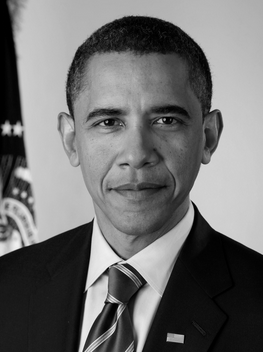
\includegraphics{figures/obama.png}}
\end{center}
\captionof{figure}{Denoising an image of President Obama with lots of salt-and-pepper noise. (a) the noisy image, (b) denoised as computed by {\tt denoise.py}, (c) denoised 2x, (d) original.}
\label{obama}
\end{marginfigure}


Let's give it a test:

\begin{lstlisting}[style=BashInputStyle]
$ python denoise.py guesswho.png
\end{lstlisting}

\noindent That should pop up the noisy Obama and the cleaned up version. You can save the cleaned up version and run {\tt denoise.py} on that one to really improve it.\sidenote[][.5in]{Hint: {\bf To save an image with PIL}, use {\tt img.save("filename.png")}.} Running {\tt denoise.py} twice, gives the cleaned up image (c) from \figref{obama}.  

\begin{callout}{\bcplume}
{\bf Deliverables}. Make sure that {\tt images/denoise.py} is correctly committed to your repository and pushed to github. 
\end{callout}

\vspace{10mm}
\section{Task 4. Re-factoring to improve code quality}

As I mentioned in the last task, {\tt blur.py} and {\tt denoise.py} are virtually identical, meaning that we have a lot of code in common. \figref{vizdiff} demonstrates this visually. One of the most important principles of computer science is to reduce code duplication. We always want exactly one place to change a particular bit of functionality.   In this case, we have the following common code:

\begin{marginfigure}
\begin{center}
\scalebox{.95}{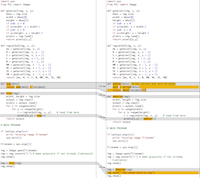
\includegraphics{figures/blur-denoise-diff.png}}
\end{center}
\caption{Visual difference between scripts {\tt blur.py} and {\tt denoise.py}. The files are identical except for orange marks.}
\label{vizdiff}
\end{marginfigure}

\begin{enumerate}
\item Functions {\tt getpixel} and {\tt region3x3}.
\item The ``main'' part of the script that loads the original image.
\item Functions {\tt blur} and {\tt denoise} are identical except for the function called to compute a new pixel in the image copy from a 3x3 region in the original ({\tt avg} or {\tt median}).
\end{enumerate}

The goal of this task is to make new versions, {\tt blur2.py} and {\tt denoise2.py}, that share as much code as possible.  The functionality will be the same, but they will be much smaller and we will get warm feeling that our code is well structured. To share code, we need to (a) put all common code in a file that these new scripts can import and (b) create a generic function called {\tt filter} that will work for both blurring and de-noising in an image. Once we get the common code into a single file, which we will call {\tt filter.py}, we can import it into {\tt blur2.py} and {\tt denoise2.py} like this:\sidenote{Do not confuse script names with function names; {\tt filter.py} can contain anything we want and it so happens that we will also put a function in there with the same name, {\tt filter}.}
 
\begin{pyverbatim}
from filter import *
\end{pyverbatim}

\noindent That statement asks Python to look in the current directory (among other places we don't care about for now) for file called {\tt filter.py} and import all of the functions. You can think of it as a formalized cut-and-paste.

Let's start by creating new ``library'' file {\tt filter.py} and placing our usual imports at the top:

\begin{pyverbatim}
import sys
from PIL import Image
\end{pyverbatim}

\noindent Now, copy functions {\tt getpixel} and {\tt region3x3} into it.

We can also create a function called {\tt open} to hide all of the messiness that checks for command-line arguments and opens the indicated image:

\begin{pyverbatim}
def open(argv):
	if len(argv)<=1:
		print "missing image filename"
		sys.exit(1)
	img = Image.open(argv[1])
	img = img.convert("L")  # make greyscale if not already (luminance)
	return img
\end{pyverbatim}

The only tricky bit\sidenote{Pun intended} is to create a single generic {\tt filter} function that can reproduce the functionality we have in functions {\tt blur} and {\tt denoise}.

\begin{enumerate}
\item Define function {\tt filter} to take {\tt img} and {\tt f} parameters.
\item Copy the body of function {\tt blur} into your new {\tt filter} function.
\item Replace the call to {\tt avg(r)} with {\tt f(r)}.
\end{enumerate}

As we discussed in class, functions are objects in Python just like any strings, lists, and so on. That means we can pass them around as function arguments.\sidenote{Don't confuse the name of a function with an expression that calls it.  Assignment {\tt f = avg} makes variable {\tt f} refer to function {\tt avg}. {\tt f = avg()} {\bf calls} function {\tt avg} and stores the return value in variable {\tt f}. Using {\tt f = avg}, we can call {\tt avg} with expression {\tt f()}. You can think of {\tt f} as an alias for {\tt avg}.} To use our new generic {\tt filter} function, we pass it an image as usual but also the name of a function:

\begin{pyverbatim}
blurred  = filter(img, avg)
denoised = filter(img, median)
\end{pyverbatim}

In the end, your {\tt filter.py} script file should have 4 functions: {\tt getpixel}, {\tt region3x3}, {\tt filter}, and {open}.

Armed with this awesome new common file, our entire {\tt blur2.py} file shrinks to a tiny script:\sidenote{You might be wondering why we don't have to include the usual {\tt sys} and {\tt PIL} imports at the start of our new files. That is because we import our {\tt filter.py} file, which in turn imports those files.}

\begin{pyverbatim}
from filter import *
# Your avg function goes here (copy from blur.py)
...
img = open(sys.argv)
img.show()
img = filter(img, avg)		# blur me please
img.show()
\end{pyverbatim}

\noindent The {\tt denoise2.py} script is also tiny:\sidenote{Yep, these files are identical except for the fact that we call {\tt filter} with different function names. If you wanted to get really fancy, you could replace both of these scripts with a single script that took a function name as a second argument (after the image filename).  With some magic incantations, you'd then ask Python to lookup the function with the indicated name and pass it to function {\tt filter} instead of hard coding.}

\begin{pyverbatim}
from filter import *
# Your median function goes here (copy from denoise.py)
...
img = open(sys.argv)
img.show()
img = filter(img, median)	# denoise me please
img.show()
\end{pyverbatim}

\begin{callout}{\bctakecare}
Before finishing this task, be a thorough programmer and test your new scripts to see that they work:
\begin{alltt}
$ python blur2.py pcb.png
$ python denoise2.py guesswho.png
\end{alltt}
They {\em should} work, but unfortunately that is never good enough in the programming world.  Lot of little things can go wrong. {\em Certainty} is always better than {\em likelihood}.
\end{callout}

We will import file {\tt filter.py} into all of our future scripts. You have created your first useful library. {\bf Good job!} \scalebox{.55}{\bcsmbh}

\begin{callout}{\bcplume}
{\bf Deliverables}. Make sure that {\tt images/blur2.py}, {\tt images/denoise2.py}, and {\tt images/filter.py} are correctly committed to your repository and pushed to github. 
\end{callout}

\vspace{10mm}

\section{Task 5. Highlighting image edges}

Now that we have some basic machinery in {\tt filter.py}, we can easily build new functionality. In this task, we want to highlight edges found within an image.  It is surprisingly easy to capture all of the important edges in an image, as shown in image (b) from \figref{jeepedges}. 

\begin{marginfigure}
\vspace{20mm}
\begin{center}
(a) \scalebox{.8}{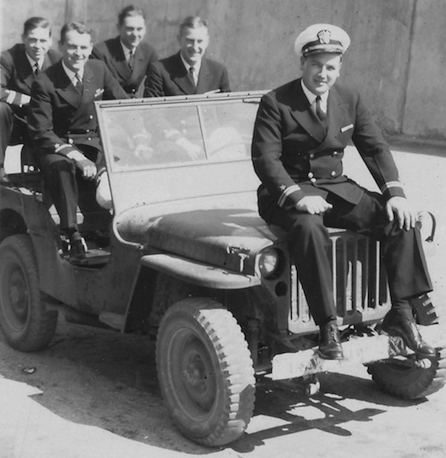
\includegraphics{figures/jeep.png}}\\
(b) \scalebox{.8}{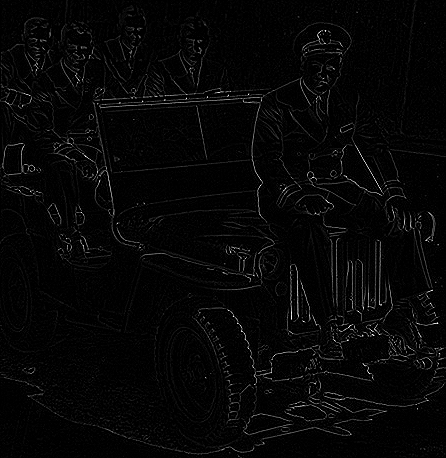
\includegraphics{figures/jeep-edges.png}}
\end{center}
\caption{Edges of an old photograph from World War II.  (a) original, (b) edges as computed by {\tt edges.py}.}
\label{jeepedges}
\end{marginfigure}

The mechanism we're going to use is derived from some serious calculus kung fu called the {\em Laplacian}, but which, in the end, reduces to 4 additions and a subtraction!  The intuition behind the Laplacian is that abrupt changes in brightness indicate edges, such as the transition from the darkness of a uniform to the brightness of a windshield edge.  As we did for blurring and denoising, we are going to slide a 3x3 region around the image to create new pixels at each {\tt x}, {\tt y}. That  means we can reuse our {\tt filter} function---we just need a {\tt laplace} function to pass to {\tt filter}.

To get started, here is the boilerplate code copied from {\tt denoise2.py} but with function name {\tt laplace} (the object of this task) passed as an argument to function {\tt filter}:

\begin{pyverbatim}
from filter import *
# define function laplace here
...
img = open(sys.argv)
img.show()
edges = filter(img, laplace)
edges.show()
\end{pyverbatim}

{\bf Create function} {\tt laplace} that takes region {\tt data} as an argument as usual. Have the function body  return the sum of the North, South, East, and West pixels minus 4 times the middle pixel from our usual region:

\begin{center}
\scalebox{.15}{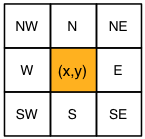
\includegraphics{figures/3x3-region.png}}
\end{center}

\noindent That computation effectively compares the strength of the current pixel with those around it.

\begin{callout}{\bcinfo}
For those familiar with calculus, we are using the second partial derivative (i.e., acceleration) in x and y directions. The first derivative would detect edges even for gradual changes but the second derivative detects only really sharp changes. For a pixel fetching function $f$ operating on a 3x3 region around $(x,y)$, ``applying the {\em Laplacian}'' means computing a filtered image pixel at $x,y$ as:

{\footnotesize $f(x + 1,y) + f(x - 1,y) + f(x,y + 1) + f(x,y - 1) - 4f(x, y)$}

where $f(x,y)$ is equivalent to our {\tt pixels[x,y]}.
\end{callout}

For example, imagine a region centered over a vertical white line. The region might look like:

\begin{center}
\scalebox{.15}{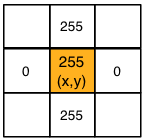
\includegraphics{figures/vertical-line-region.png}}
\end{center}

\marginnote{Be aware of something that Pillow is doing for us automatically when we store values into an image with {\tt pixels[x,y] = v}.  {\bf If {\tt v} is out of range 0..255, Pillow clips {\tt v}}. So, for example, {\tt pixels[x,y] = -510} behaves like {\tt pixels[x,y] = 0} and {\tt pixels[x,y] = 510} behaves like {\tt pixels[x,y] = 255}. It doesn't affect edge detection or any of our other operations in future tasks but I wanted to point out that in a more advanced class we would {\bf scale} these pixel values instead of clipping them. Clipping has the effect of reducing contrast.
}

\noindent The {\tt laplace} function would return $255+255+0+0 - 4 \times 255 = -510$. 

Compare that to the opposite extreme where values are almost the same:

\begin{center}
\scalebox{.15}{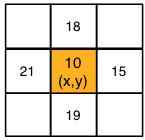
\includegraphics{figures/flat-region.png}}
\end{center}

\noindent The {\tt laplace} function would return $18+19+15+21 - 4 \times 10 = 33$.

Once you have implemented your {\tt laplace} function, give it a try with some of the sample images you have such as the jeep or Obama:

\begin{lstlisting}[style=BashInputStyle]
$ python edges.py obama.png
\end{lstlisting}

It actually does a really good job capturing Obama's outline:\\
~\\

\begin{minipage}{\linewidth}
\makebox[\linewidth]{%
\scalebox{.3}{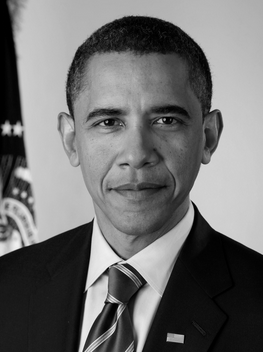
\includegraphics{figures/obama.png}} \scalebox{.3}{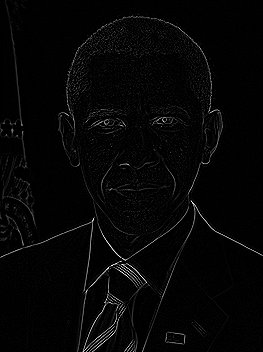
\includegraphics{figures/obama-edges}}
}
\end{minipage}

\begin{callout}{\bcplume}
{\bf Deliverables}. Make sure that {\tt images/edges.py} is correctly committed to your repository and pushed to github. 
\end{callout}

\section{Task 6. Sharpening}

Sharpening an image is a matter of highlighting the edges, which we know how to compute from the previous tasks. Script {\tt edges.py} computes just the edges so, to highlight the original image, we {\em subtract} that white-on-black edges image from the original.  You might imagine that {\em adding} the edges back in would be more appropriate and it sort of works, but the edges are slightly off. We get a better image by subtracting the high-valued light pixels because that darkens the edges in the original image, such as between the uniform and the windshield. Let's start with the easy stuff:

\begin{marginfigure}
\begin{center}
(a) \scalebox{.6}{
\includegraphics{figures/bonkers-bw-zoom.png}}\\
(b) \scalebox{.6}{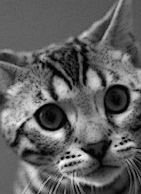
\includegraphics{figures/bonkers-sharp-zoom.png}}
\end{center}
\caption{Bonkers the cat portrait. (a) original and (b) sharpened as computed by {\tt sharpen.py}.}
\label{jeepedges}
\end{marginfigure}

\begin{enumerate}
\item Copy your previous {\tt edges.py} file to new script {\tt sharpen.py}.
\item After {\tt edges = filter(img, laplace)}, add a line that calls a function we'll create shortly called {\tt minus}. {\tt minus} takes two image parameters, {\tt A} and {\tt B} and returns {\tt A-B}.  In our case, pass in the original image and the image you get back from calling {\tt filter(img, laplace)}.
\item Show the result of the {\tt minus} function.
\end{enumerate}

That only leaves the task of {\bf creating function} {\tt minus} to subtract the pixels of one image from the pixels of another image like a 2-D matrix subtraction.  As we did before, we will return a modified version of a copy of an incoming image parameter. (In my solution, I arbitrarily chose to create and return a copy of {\tt A}.) Because you are getting really good at creating functions to manipulate images, the instructions for creating {\tt minus} in this  task are less specific than in previous tasks.  You need to fill in the body of this function:
 
\begin{pyverbatim}
# Return a new image whose pixels are A[x,y] - B[x,y]
def minus(A, B):
	...
\end{pyverbatim}

The mechanism is the same as before: iterating loop variables {\tt x} and {\tt y} across the entire image and processing the pixel at each location. The only difference between this function and {\tt filter} is that we want to operate on individual pixels not 3x3 regions.  In the inner loop, set {\tt pixels[x,y]} to the value of pixel {\tt A[x,y]} minus pixel {\tt B[x,y]}. Don't forget to return the image you filled in.

Here's how to run {\tt sharpen.py} on Bonkers the cat:

\begin{lstlisting}[style=BashInputStyle]
$ python sharpen.py bonkers-bw.png
\end{lstlisting}

\noindent \figref{bonkers3}, \figref{phobos3}, and \figref{jeep3} show some sample transformation sequences with original, {\em Laplacian}, and sharpened images.

\begin{callout}{\bcplume}
{\bf Deliverables}. Make sure that {\tt images/sharpen.py} is correctly committed to your repository and pushed to github. Tag when completed with {\tt images}. 
\end{callout}

\begin{minipage}{0.8 \linewidth}
\makebox[\linewidth]{%
\scalebox{.35}{
\includegraphics{figures/bonkers-bw-zoom.png}} \scalebox{.35}{
\includegraphics{figures/bonkers-edges-zoom.png}} \scalebox{.35}{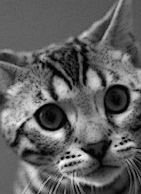
\includegraphics{figures/bonkers-sharp-zoom.png}}
}
\captionof{figure}{Sharpening of a Bonkers the cat. Clockwise: (a) original, (b) edges as computed by {\tt edges.py}, (c) the sharpened image as computed by {\tt sharpen.py}.}
\label{bonkers3}
\end{minipage}

\begin{minipage}{0.8 \linewidth}
\makebox[\linewidth]{%
\scalebox{.45}{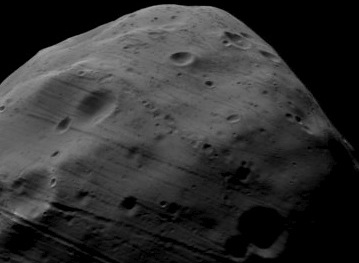
\includegraphics{figures/phobos1.png}}
\scalebox{.45}{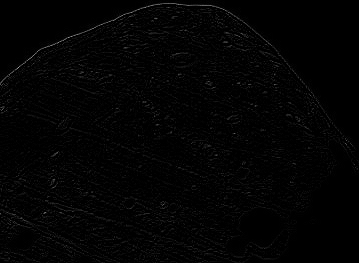
\includegraphics{figures/phobos1-edges.png}}\\
\scalebox{.45}{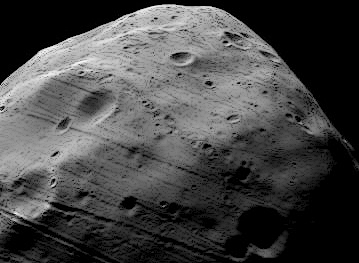
\includegraphics{figures/phobos1-sharp.png}}
}
\captionof{figure}{Sharpening of Phobos asteroid from NASA. Clockwise: (a) original, (b) edges as computed by {\tt edges.py}, (c) the sharpened image as computed by {\tt sharpen.py}.}
\label{phobos3}
\end{minipage}

\begin{minipage}{0.8 \linewidth}
\makebox[\linewidth]{%
\scalebox{.45}{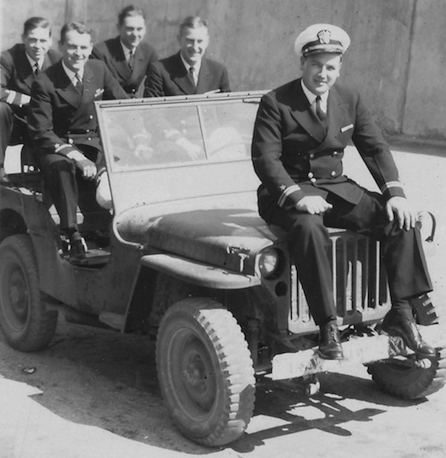
\includegraphics{figures/jeep.png}}
\scalebox{.45}{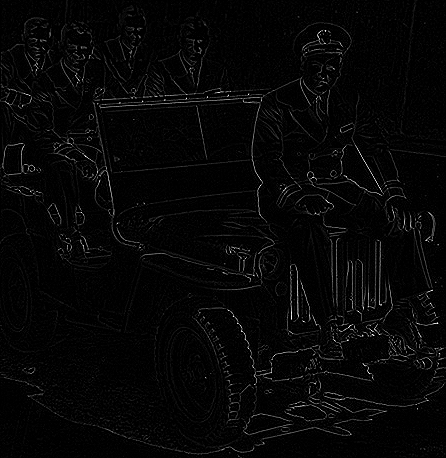
\includegraphics{figures/jeep-edges.png}}\\
\scalebox{.45}{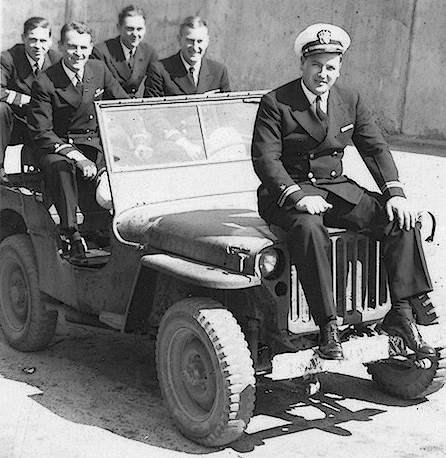
\includegraphics{figures/jeep-sharp.png}}
}
\captionof{figure}{Sharpening of an old photograph from World War II. Clockwise: (a) original, (b) edges as computed by {\tt edges.py}, (c) the sharpened image as computed by {\tt sharpen.py}.}
\label{jeep3}
\end{minipage}



\chapter{Histograms Using {\tt matplotlib}}

{\bf TODO: reuse runif() from previous project for 2015}.

\setcounter{problem}{1}
\section{Discussion}

\begin{fullwidth}

The goal of this lab is to teach you the basics of using matplotlib to display probability mass functions, otherwise known as histograms. In this lab we will use the uniform distribution. Use filename {\tt hist.py}.

\section{Steps}

\step import the proper libraries

\begin{pyverbatim}
import matplotlib.pyplot as plt
import numpy as np
\end{pyverbatim}

\step Get a sample of uniform random variables in $U(0,1)$

\begin{pyverbatim}
N = 1000
X = [np.random.uniform(0,1) for i in range(N)] # U(0,1)
# or np.random.uniform(0,1,N)
\end{pyverbatim}

\step Display a histogram using matplotlib (in a separate window)

\begin{pyverbatim}
plt.hist(X, normed=1)
plt.show()
\end{pyverbatim}

\step Run it. \\

\step Now, save the image as a PDF to the same directory by inserting a save command in between the histogram and the show method:

\begin{pyverbatim}
plt.hist(X, normed=1)
plt.savefig('unif-0-1-density.pdf', format="pdf")
plt.show()
\end{pyverbatim}

\step Run it. Your pdf file should look like

\scalebox{.25}{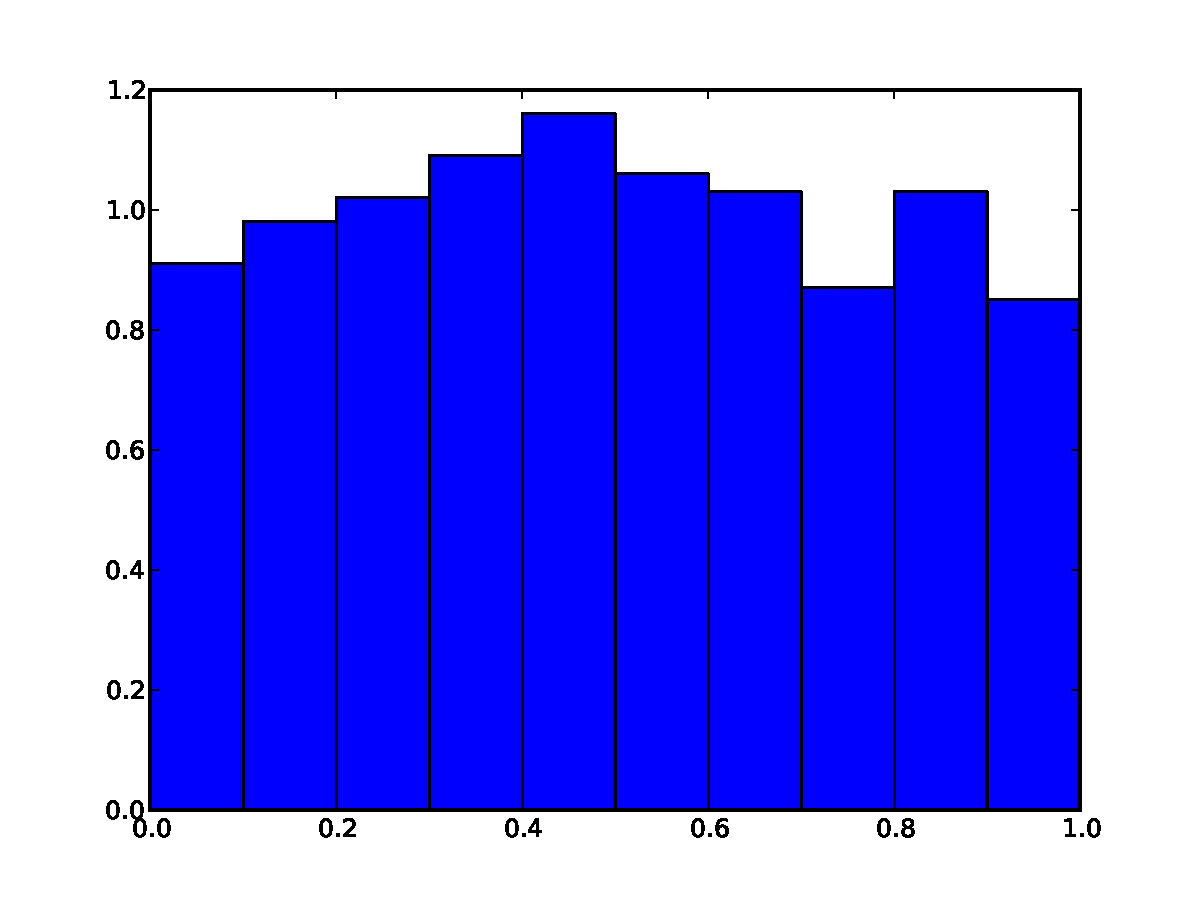
\includegraphics{figures/unif-0-1-density.pdf}}

\step  Graphs should always have the axes labeled. Let's do that as well as add a title and set the range of the graph. Put this code right before the {\tt savefig()}.

\begin{pyverbatim}
plt.title("U(0,1) Density Demo")
plt.xlabel("X", fontsize=16)
plt.ylabel("Density", fontsize=16)
plt.axis([0, 1, 0, 2])
\end{pyverbatim}

\step Run it. \\

\step It's also common to add some annotations inside the graph to explain more about what we are seeing. First, we need to get access to the figure itself and then has to figure about its axes. (We need this in order to specify coordinates within the graph.) Put the following code before the {\tt hist()} call.

\begin{pyverbatim}
fig = plt.figure()        # get a handle on the figure object itself
ax = fig.add_subplot(111) # weird stuff to get the Axes object within figure
\end{pyverbatim}

Then, before the {\tt savefig()},  add the following to display some text above the histogram within the graph. The coordinates are from 0..1 where 0 is the left/bottom edge and 1 is the right/top edge.

\begin{pyverbatim}
# put N=... at top left
plt.text(.1,.9, 'N = %d' % N,
		 fontsize=16,
		 transform = ax.transAxes) 
\end{pyverbatim}

\step Also, let's change the file name slightly so we can keep our original graph plus our fancy one:

\begin{pyverbatim}
plt.savefig('unif-0-1-density-fancy.pdf', format="pdf")
\end{pyverbatim}

\step Run it. \\

\scalebox{.25}{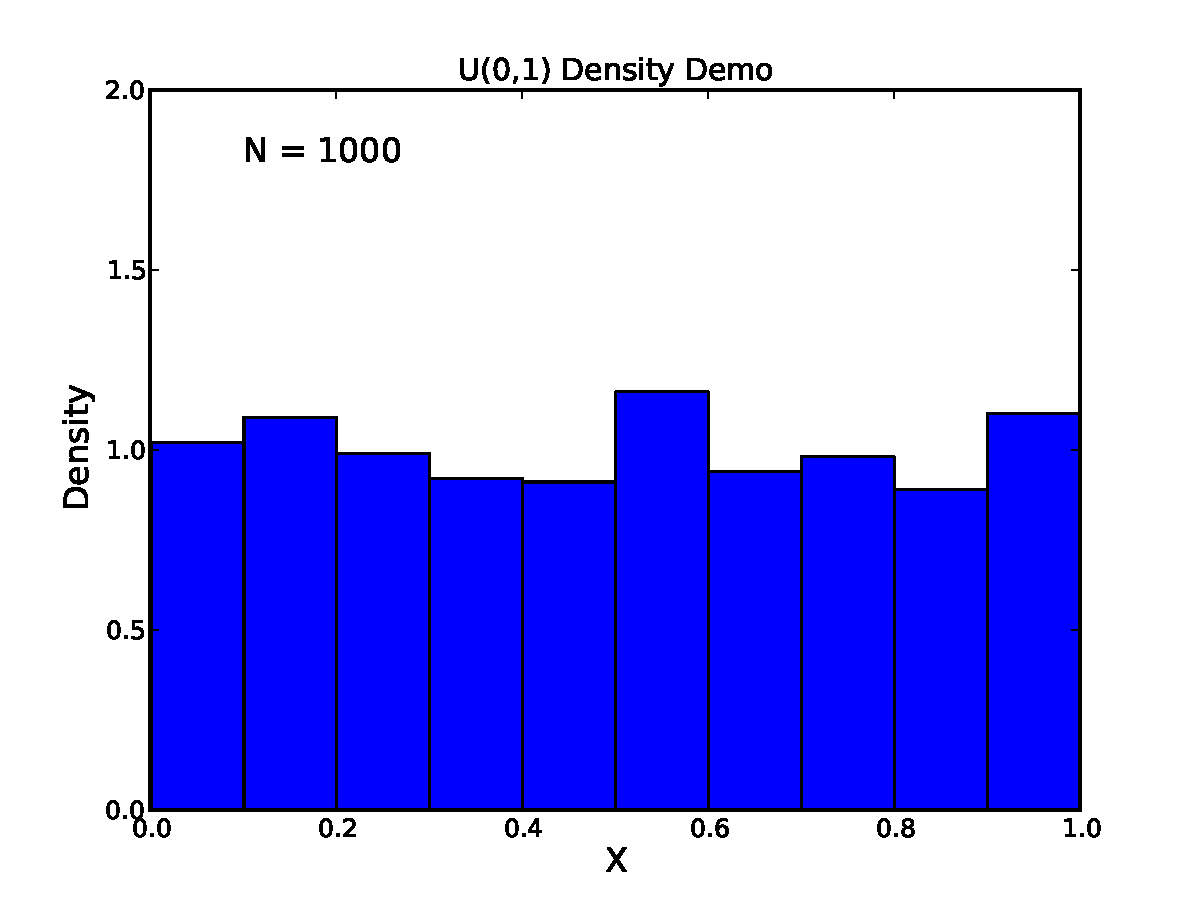
\includegraphics{figures/unif-0-1-density-fancy.pdf}}

{\bf To understand distributions, it's a great idea to start messing around with the parameters of the density or mass function.} \\

\step Change $U(0,1)$ to $U(2,8)$ and examine the results. You will have to alter the axis() to use different ranges. (Or let the plotting software do the work for you and get rid of the axis() call.) Run it. You should see something like the following.

\scalebox{.25}{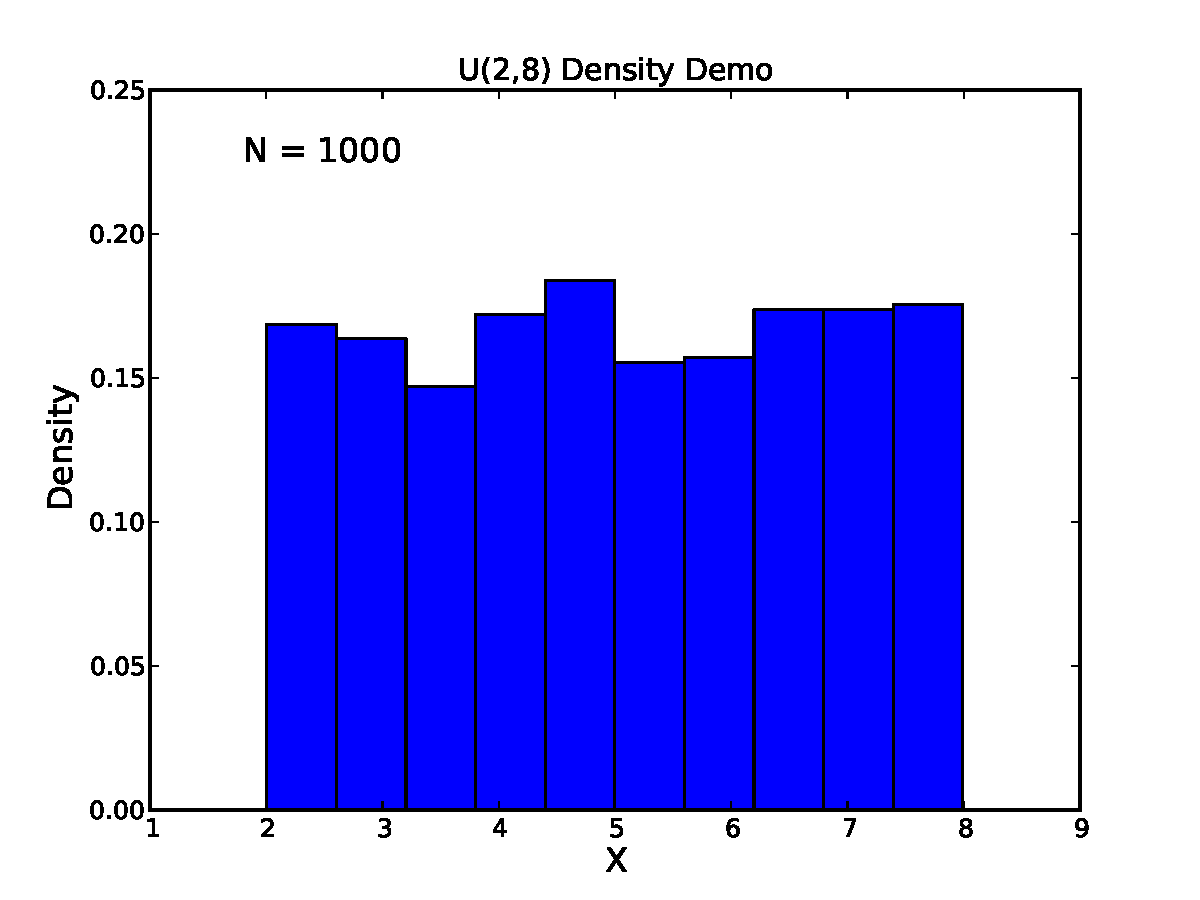
\includegraphics{figures/unif-2-8-density-fancy.pdf}}

\section{Deliverables}

Please submit:

\begin{itemize}
\item your {\tt hist.py} Python file
\item a PDF of your $U(2,8)$ graph.
\end{itemize}

\end{fullwidth}

\chapter{Graph Adjacency Lists and Matrices}

\setcounter{problem}{1}

\section{Goal}

\begin{fullwidth}

The goal of this task is to teach you about the implementation of graphs in Python, how to implement a few simple related algorithms, and do some simple data loading.  As part of this exercise, you will also learn to transform data, which is an important data preparation skill you will need as an analyst. 

\section{Discussion}

In this project, you will convert a \href{https://raw.githubusercontent.com/parrt/msan501/master/data/graph}{{\textcolor{blue}string representation of a graph}} that looks like this:

\begin{alltt}\small
parrt: tombu, dmose, parrt
tombu: dmose, kg9s
dmose: tombu
kg9s: dmose
\end{alltt}

\noindent to an adjacency list representation and ultimately generate a visual representation via \href{http://www.graphviz.org/}{\textcolor{blue}{graphviz/dot}}:

\begin{center}
\scalebox{.55}{\includegraphics{figures/email-graph.pdf}}
\end{center}

\noindent For fun, you will also create an edge matrix representation:

\[
\bordermatrix{
~ & parrt & tombu & dmose & kg9s \cr
parrt & 1 & 1 & 1 & 0\cr
tombu & 0 & 0 & 1 & 1 \cr
dmose & 0 & 1 & 0 & 0 \cr
kg9s & 0 & 0 & 1 & 0\cr
}
\]

\noindent where the nodes have the following indexes (all we really care about here is the order):
 
\[
\left[
\begin{array}{c}
0: parrt \\
1: tombu \\
2: dmose \\
3: kg9s \\
\end{array}
\right]
\]

The following sections describe the functions you must create in {\tt graphs.py}. Your starter kit should have some boilerplate code set up for you.

\subsection{Processing an adjacency list string}

First, you have to process a string representation of an adjacency list and create an internal data structure:

\begin{pyverbatim}
def adjlist(adj_list):
    """
    Read in adj list and store in form of dict mapping node
    name to list of outgoing edges. Preserve the order you find
    for the nodes.
    """
    ...
\end{pyverbatim}

You will use an ordered dictionary ({\tt OrderedDict}) that maps node name x to a list of target nodes. x will be a string and the target list will be a list of strings. For example, from line in string adj\_list

\begin{alltt}
parrt: tombu, dmose, parrt
\end{alltt}

\noindent you will create an entry in the dictionary with key {\tt parrt} and value:

\begin{pyverbatim}
['tombu', 'dmose', 'parrt']
\end{pyverbatim}

\noindent To process the text, you must split the incoming string into lines and then process them one at a time as each line represents an adjacency list. You will use string functions {\tt split} and (likely) {\tt strip} to process the text. The goal here is to learn how to process text so don't look for built-in functions that do all of this for you.

\noindent Printing the adjacency list dictionary from {\tt adjlist}, we should all get the following output:

\begin{pyverbatim}
OrderedDict([('parrt', ['tombu', 'dmose', 'parrt']),
 ('tombu', ['dmose', 'kg9s']), 
 ('dmose', ['tombu']), 
 ('kg9s', ['dmose'])])
\end{pyverbatim}

\subsection{Adjacency list to adjacency matrix}

Given an adjacency list stored as a dictionary per adjlist(), create a function that converts it to an adjacency matrix:
 
\begin{pyverbatim}
def adjmatrix(adj):
    """
    From an adjacency list, return the adjacency matrix with entries in {0,1}.
    The order of nodes in adj is assumed to be same as they were read in.
    """
    ...
\end{pyverbatim}

\noindent The matrix should look like the one shown above.

\subsection{Getting a list of all nodes}

A very useful function to have is the following that returns a list of all nodes visited starting at a particular node in a graph. 
 
\begin{pyverbatim}
def nodes(adj, start_node):
    """
    Walk every node in graph described by adj list starting at start_node
    using a breadth-first search.  Return a list of all nodes found (in
    any order). Include the start_node.
    """
    ...
\end{pyverbatim}

\noindent Do not build a recursive function as you must do a breadth-first search. (Recursive functions are much more useful when doing a depth-first search.) The basic algorithm looks like this:

\begin{algorithm}[H]
\SetInd{.3em}{.3em}
$visited$ = []\;
add the start node to a work list\;
\While{more work}{
    node = remove a node from work list\;
    add node to $visited$ list\;
    targets = adjacency\_list[node]\;
    add all unvisited targets to work list\;
}
\Return{visited}\;
\end{algorithm}

\subsection{Generating DOT output}

In order to visualize the graph you have read in, create the following function that dumps valid Graphviz DOT code, given an adjacency list. Then cut-and-paste the output and put it into Graphviz to display it.
 
\begin{pyverbatim}
def gendot(adj):
    """
    Return a string representing the graph in Graphviz DOT format
    with all p->q edges. Parameter adj is an adjacency list.
    """
    ...
\end{pyverbatim}

\noindent Or, to amaze your family and friends, you can directly from the command line on a mac or unix box:

\begin{lstlisting}[style=BashInputStyle]
$ python test_dot.py | dot -Tpdf > /tmp/graph.pdf; open /tmp/graph.pdf
\end{lstlisting}

Here is a simple test rig, {\tt test\_dot.py}, that translates an input string description to DOT and prints it out.

\begin{pyverbatim}
from graph import *

# test dot
g = \
"""
parrt: tombu, dmose, parrt
tombu: dmose, kg9s
dmose: tombu
kg9s: dmose
"""
list = adjlist(g)
dot = gendot(list)
print dot
\end{pyverbatim}

\noindent For the adjacency list shown at the start of this assignment, you should to generate the following DOT code:

\begin{alltt}\small
digraph g \{
  rankdir=LR;
  parrt -> tombu;
  parrt -> dmose;
  parrt -> parrt;
  tombu -> dmose;
  tombu -> kg9s;
  dmose -> tombu;
  kg9s -> dmose;
\}
\end{alltt}

\section{Testing}

I have provided {\tt test\_graphs.py} and {\tt test\_dot.py}  test rigs that exercise the required functions using the sample adjacency list described above. Please make sure that your library works with this test rig.

\section{Real data}

{\bf EXTRA CREDIT}

And, now, let's try something real though still pretty small. Get the \href{http://www-personal.umich.edu/~mejn/netdata/adjnoun.zip}{\textcolor{blue}{Word adjacencies in the book David Copperfield}} as a graph in {\tt .gml} (graph modeling language) format from M. E. J. Newman, {\em Finding community structure in networks using the eigenvectors of matrices}, Preprint physics/0605087 (2006). Visually, the graph looks like this:

\begin{center}
\scalebox{.35}{\includegraphics{figures/wordgraph-zoom.pdf}}
\end{center}

\noindent Or, in its full glory:

\begin{center}
\scalebox{.55}{\includegraphics{figures/wordgraph.pdf}}
\end{center}

You will need to install package NetworkX to read in the graph modeling language file format:

\begin{lstlisting}[style=BashInputStyle]
$ sudo pip install NetworkX
\end{lstlisting}

\noindent The data looks like this in text format:

\begin{alltt}\small
Creator "Mark Newman on Fri Jul 21 13:00:02 2006"
graph
[
  node
  [
    id 0
    label "agreeable"
    value 0
  ]
  node
  [
    id 1
    label "man"
    value 1
  ]
...
  edge
  [
    source 32
    target 15
  ]
...
\end{alltt}

(By the way, I had to install NetworkX and pyparsing within PyCharm because it did not see the {\tt pip} installations I did from the command line.)

You must create {\tt wordgraph.py} that reads accepts a .gml file as a commandline argument (i.e., our downloaded {\tt adjnoun.gml} file), converts it to an adjacency list with a {\tt gml2adjlistt()} function, and then generates DOT with your {\tt gendot()} function. Make sure to keep the same order in the adjacency list you create as found in the .gml file.  Here is the boilerplate function in the {\tt wordgraph.py} starter kit in the repository:

\begin{pyverbatim}
def gml2adjlist(G):
    """
    Return a dict mapping word to adjacent nodes. G.node dict in memory
    looks like:

    {0: {'id': 0, 'value': 0, 'label': 'agreeable'},
    1: {'id': 1, 'value': 1, 'label': 'man'}, ... }

    and G.edge dict looks like:

    {0: {1: {}, 2: {}, 3: {}}, 1: {0: {}, 19: {}, 2: {}, 102: {}, ...}, ...}

    and we need:

    {agreeable:['man', 'old', 'person'], man:[['agreeable', 'best', 'old', ...], ...}
    """
    words = collections.OrderedDict()  # keep stuff in order read from GML
    ...
    return words
\end{pyverbatim}

The code is not too tricky, but you have to figure out how to extract the {\tt label} from each node to get the node list. The edges start out as node ids not words so you need to convert those to words in order to create an appropriate adjacency list.

Save the DOT output to a file and compare it to the {\tt wordgraph.dot} file I provide in the repository. I.e., the following command should generate no output because there should be no difference between the files:

\begin{lstlisting}[style=BashInputStyle]
$ diff wordgraph.dot yourfile.dot
\end{lstlisting}

\begin{callout}{\bcplume}
{\bf Deliverables}. Make sure that {\tt graphs/graphs.py} (the functions inside should emit no output at all, just return data as specified), {\tt graphs/wordgraph.py} are correctly committed to your repository and pushed to github. Tag when completed with {\tt graphs}.
\end{callout}

\end{fullwidth}


\part{Empirical statistics}

\chapter{``Newbies say the darndest things''}

\begin{fullwidth}
{\em in progress.  warnings for newbies.}

-1/2 is -1 and 1/2 is 0 in Python.  There is no automatic promotion when you send an integer to a function that is expecting a floating-point number.

(-1/lambduh)*(np.log(1-u)) vs -(np.log(1-u))/lambduh. The latter is probably better because it does fewer floating-point operations and hence probably has fewer errors.

\end{fullwidth}

\chapter{Computing Point Statistics}

\setcounter{problem}{1}
\section{Discussion}

\begin{fullwidth}

The goal of this task is to refresh your memory of a few point statistics. 

\subsection{Stats}

This exercise involves writing functions to compute sample mean, variance, and covariance from a data set (list of values).  In mathematics notation, the sample estimates are:

\[\tag{Sample mean}
\bar x = \frac{1}{N} \sum_{i=1}^{N} x_i 
\]

\[\tag{Unbiased sample variance}
s^2 = \frac{1}{N-1} \sum_{i=1}^{N} (x_i - m)^2
\]

\[\tag{Unbiased sample covariance}
cov(x,y) = \frac{1}{N-1} \sum_{i=1}^{N} (x_i - \bar x)(y_i - \bar y)
\]

In Python, you must define functions {\tt mean(x)}, {\tt var(x)}, {\tt cov(x,y)} where {\tt x} and {\tt y} are objects that behave like a list or iterator. The functions return a floating-point value based on the above mathematics notation. If the length of the incoming vectors to {\tt cov} are not the same, return 0. 

\subsection{Libraries}

While we're at it let's learn about creating and importing our own libraries.  You'll notice that {\tt test\_point\_stats.py} references your code like this:

\begin{pyverbatim}
from stats import *
\end{pyverbatim}

\noindent That lets us directly access the functions defined in the {\tt stats.py} file you are going to create.
 
You can test the correctness of the functions by using the {\tt numpy} lib, make sure you ask for the sample population statistics by using parameter {\tt ddof=1} for {\tt var()} and {\tt cov()}. E.g., {\tt np.var(data, ddof=1)}. Be careful not to confuse function names; e.g., {\tt numpy} has functions with the same names (although cov() returns a covariance matrix).

\begin{pyverbatim}
import numpy as np  # np is an alias for the numpy library
x = ...
y = ...
print np.cov(x,y)[0][1] # np.cov returns cov matrix
\end{pyverbatim}

We now have the kernel of a small statistics library in {\tt stats.py} and we will continue to add functions to this as we go along. 

\subsection{Testing}

In computer science, programmers recognize two primary kinds of tests: {\em unit tests} and {\em functional tests}. A unit test is really just testing a function or a few functions whereas functional tests test the overall functionality of the program. In file {\tt test\_point\_stats.py}, I have provided a set of unit tests that you can use for basic sanity checking of your project. 

To make the unit tests work, make sure that you install \href{http://pytest.org/latest/getting-started.html}{py.test}, which is usually just a matter of:

\begin{alltt}
easy_install -U pytest
\end{alltt}

Test your code using the following command line (with your {\tt stats.py} is in the same directory):

\begin{lstlisting}[style=BashInputStyle]
$ python -m pytest test_point_stats.py
============================= test session starts ==============================
platform darwin -- Python 2.7.6 -- py-1.4.30 -- pytest-2.7.2
rootdir: /Users/parrt/msan501/stats, inifile: 
collected 3 items 

test_point_stats.py ...
=========================== 3 passed in 0.01 seconds ===========================
\end{lstlisting}

\noindent If you don't see all tests passing, and there is a problem at a basic level with your software.

\begin{callout}{\bctakecare}
You may not use sum() or any other built-in functions for this project to compute the point statistics.  The whole point of the exercise is to learn to build your own for loops. Obviously.
\end{callout}

\begin{callout}{\bcplume}
{\bf Deliverables}. Make sure that {\tt stats/stats.py} (the functions inside should emit no output at all, just return data as specified) is correctly committed to your repository and pushed to github. 
\end{callout}


\end{fullwidth}


\chapter{Approximating $\sqrt{n}$ with the Babylonian Method}

\setcounter{problem}{1}
\section{Motivation}

\begin{fullwidth}

This lab is really a fancy way to learn about looping in Python and how to quickly prototype something in Excel (if warranted). It also gets you used to encoding mathematical expressions and recurrence relations in Python.
 
\section{Discussion}

To approximate square root, $\sqrt{n}$, the idea is to pick an initial estimate, $x_0$, and then iterate with better and better estimates, $x_{i}$, using the recurrence relation:

\[
x_{i+1} = \frac{1}{2} (x_i + \frac{n}{x_i})
\]

To see how this works, jump into Excel (yes, a spreadsheet) and crank through a few iterations by defining cells with $n$ and your initial estimate $x_0$, which can be anything you want. (It's sometimes easier to play around without having to deal with a programming language.) Then you need to define a cell that computes the above better approximation using $x_i$ as the cell above it. I hardcoded the names in column A and the first two rows of column B. Cell B3 should be a formula that computes B4 based upon B3. Then you can extend the formula down and watch it converge on the final (correct) value for $\sqrt{125348}$. My spreadsheet looks like this:

~\\
\scalebox{.25}{\includegraphics{figures/sqrt-excel.pdf}}
~\\

Try out any nonnegative number and you'll see that it still converges, though at different rates.

There's a great deal on the web you can read to learn more about why this process works but it relies on the average (midpoint) of $x$ and $n/x$ getting us closer to $\sqrt{n}$.  It can be shown that if $x$ is above $\sqrt{n}$ then $n/x$ is below $\sqrt{n}$ and the reverse is true if $x$ is below the root.  The iteration converges and does so quickly. Informally, as shown in Wikipedia, we can represent the true square root by adding an error term to our estimate:

\[
\sqrt{n} = x + \epsilon
\]

or,

\[
n = (x + \epsilon)^2
\]

Expanding, we get:

\[
n = x^2 + 2x\epsilon + \epsilon^2
\]

Solving for $\epsilon$:

\[
n - x^2 = \epsilon (2x + \epsilon)
\]

\[
\epsilon = \frac{n - x^2}{2x + \epsilon}
\]

Because $\epsilon$ is much smaller than $x$, we can drop it from the denominator leaving us with an estimate of epsilon:

\[
\epsilon = \frac{n - x^2}{2x}
\]

Then we can plug it back into $x + \epsilon$ and get:

\[
x := x + \epsilon = x + \frac{n - x^2}{2x} = \frac{2x^2}{2x} + \frac{n - x^2}{2x} = \frac{1}{2}\frac{x^2 + n}{x} = \frac{1}{2}(x + \frac{n}{x})
\]

Which gets its back to the Babylonian formula. Since we dropped an $\epsilon$ term, this formula for $x$ is inexact but it gets us closer to $\sqrt{n}$.

\cut{
To play first use Excel: 
=0.5*(B2+\$B\$1/B2)
}

Now that you understand how this estimate works, your goal is to implement a simple Python method called sqrt() that uses the Babylonian method to approximate the square root. Here is a starter kit for you. Please call the file {\tt sqrt.py}.

\begin{alltt}\small
import math

# Stop iterating when the new approximation is within
# PRECISION of the old value.
PRECISION = 0.000001

# compute square root of n
def sqrt(n):
    x_0 = 1.0 # pick any old value
    ... fill this in ...

def check(n):
    delta = math.sqrt(n) - sqrt(n)
    if delta > PRECISION:
        raise BaseException("Inaccurate sqrt(%f)=%f; estimate is %f" %
            (n, math.sqrt(n), sqrt(n)))

# check a range of values
check(125348)
check(100)
check(1)
check(0)
\end{alltt}

\section{Deliverables}

Please submit:

\begin{itemize}
\item a PDF showing a snapshot of your spreadsheet
\item the formula you used in B3 {\bf and} B4.
\item your {\tt sqrt.py} Python file
\end{itemize}

\end{fullwidth}

\chapter{Uniform Random Number Generation}

\setcounter{problem}{1}

\begin{quote}
{\bf Q}: {\em How to generate pure random string}? \\
{\bf A}: {\em Put a fresh student in front of vi editor and ask him to quit}.\\
~~~~--- Emiliano Lourbet (@taitooz)
\end{quote}

\section{Discussion}

\begin{fullwidth}

To perform computer-based simulation we need to be able to generate random numbers. Generating random numbers following a uniform distribution are the easiest to generate and are what comes out of the standard programming language ``give me a random number'' function.  Here's a sample Python session:

\begin{pyconsole}
import random
print random.random()
print random.random()
print random.random()
\end{pyconsole}

We could generate real random numbers by accessing, for example, noise on the ethernet network device but that noise might not be uniformly distributed. We typically generate pseudorandom numbers that aren't really random but look like they are. From Ross' {\em Simulation},  we see a very easy recursive mechanism that generators values in $[0,m-1]$:\\

$x_n = a x_{n-1}$ modulo $m$\\

That's recursive (or iterative and not {\em closed form}) because $x_n$ is a function of a prior value: \\

\noindent $x_1 = ax_0$ modulo $m$\\
$x_2 = ax_1$ modulo $m$\\
$x_3 = ax_2$ modulo $m$\\
$x_4 = ax_3$ modulo $m$\\
$...$\\

\noindent To get random numbers between 0 and 1, we use $x_n / m$.

We must pick a value for $a$ and $m$ that make $x_n$ seem random. Ross suggests choosing a large prime number for $m$ that fits in our integer word size, e.g., $m = 2^{31} - 1$, and $a = 7^5 = 16807$.

Initially we set a value for $x_0$, called the {\em random seed} (it is not the first random number). Every seed leads to a different sequence of pseudorandom numbers. In Python, you can set the seed of the standard library by using {\tt random.seed([x])}.

Your goal is to take that simple recursive formula and use it to generate the first 10 random numbers using a {\tt for} loop in Python. Use $m = 2^{31} - 1$, $a = 7^5 = 16807$, and an initial seed of $x_0 = 666$.  Your output should look something like:

%import code.runif

\begin{verbatim}
0.00521236192678
0.604166903349
0.233144581892
0.460987861017
0.822980116505
0.826818094508
0.331714398848
0.1239014343
0.411406287184
0.505468696591
\end{verbatim}

Because we are all using the same seed, the sequence of numbers should be the same.

\section{Deliverables}

You must turn in a printout of your python script and your output.

\end{fullwidth}

\chapter{Generating Binomial Distributions}

\setcounter{problem}{1}
\section{Discussion}

\begin{fullwidth}

The goal of this lab is to simulate a binomial distribution using repeated Bernoulli trials and then compare it against the theoretical binomial distribution. Use filename {\tt rbinomial.py}.

\step First, set the seed of the random number generator. Otherwise you will always get the same  Bernoulli trials. In this case, we're using the current time in milliseconds as the random seed so that it is different every time you run the program. (remember this trick.)

\begin{pyverbatim}
np.random.seed( int(round(time.time() * 1000)) )
\end{pyverbatim}

\step Next, define a function that performs $n$ Bernoulli trials with probability $p$ of success. It should return the number of successes, $k$, out of $n$:

\begin{pyverbatim}
def binomial(n,p):
    "Sim with prob p, n bernoulli trials; return number of successes"
    ...
\end{pyverbatim}

The pseudocode is just a loop that goes around $n$ times and uses a variable from $U(0,1)$ to check for success or failure. For example, my solution assumes failure if the uniform random variable is greater than $p$.
    
\step Get list $X$ as $N$ Bernoulli trials with parameters $N=500$ and $P=0.4$. Do that by simply calling the {\tt bernoulli} function $N$ times.

\step Plot the histogram normalized (normed=1) and run it. you should see the following:

\scalebox{.35}{\includegraphics{figures/rbinomial-500-4.pdf}}

\step We could use the built-in binomial mass function but let's define our own since it's easy:

\[\tag{Binomial mass function}
\binom{n}{k} p^k (1-p)^{n-k}
\]

\noindent That's the probability that there are $k$ successes in $n$ trials with probability $p$ of success. Define a function like this:

\begin{pyverbatim}
def binom(k, n, p):
    """
    If we run n trials with p prob for each trial of success,
    how many have k successes?
    """
    ...
\end{pyverbatim}

\step To show the real distribution on top, we need to iterate $k$ across the range $0..N$ used in our empirical test above.  Since this is a mass function not a smooth density function, we can use every fifth value in the range. Let's also add some text to describe the parameters.

\begin{pyverbatim}
y = [binom(k, N, P) for k in range(0,N+1,5)]
plt.bar(range(0,N+1,5), y, color='red', align='center', width=1)
plt.axis([150,250,0,.05]) # set the axes so that we get a close-up
plt.text(160,0.04, '$N = %d$' % N, fontsize=16)
plt.text(160,0.037, '$P = %f$' % P, fontsize=16)
\end{pyverbatim}

In this case I am not using 0..1 for the axes coordinates of the text; the default is the values of the graph itself. sometimes this is useful.

\step Run it and you should see something like the following:

\scalebox{.35}{\includegraphics{figures/rbinomial-500-4-fancy.pdf}}

Note that we use a bar chart for the binomial theoretical distribution and not a smooth graph because this is a mass function not a density function.

\section{Deliverables}

Please submit:

\begin{itemize}
\item your {\tt rbinomial.py} file
\item submit a PDF of your final graph.
\end{itemize}

\end{fullwidth}

\chapter{Generating Exponential Random Variables}

\setcounter{problem}{1}
\section{Discussion}

\begin{fullwidth}

The goal of this lab is to generate random values from the exponential distribution using the inverse transform method.  You will show the histogram of the random values and then show the theoretical exponential distribution on top to verify your results. You will reuse your exponential distribution random variable generator for the central limit theorem lab. Use filename {\tt rexp.py}.

\section{Steps}

\step First, create a function called {\tt rexp(lambduh)} that returns a random value from the exponential distribution using the inverse transform method. To do that, you need the inverse {\em cumulative distribution function} (CDF) for the exponential distribution $Exp(\lambda)$. The {\em probability density function} for the exponential distribution is:

\[
p = F(x; \lambda) = \lambda e^{-\lambda x}
\]

\noindent Therefore the inverse function to get the $x$ value associated with a probability $p$, we use

\[
x = F^{-1}(p; \lambda) = -\frac{ln(1-p)}{\lambda}
\]

\noindent Your function should look like the following:

\begin{pyverbatim}
def rexp(lambduh): # lambduh mispelled to avoid clash with lambda in python
    # u = get value from U(0,1) then
    # return F^-1(u) for exp cdf F^-1
\end{pyverbatim}

\noindent Use your {\tt runif()} function from previous labs.

\step To plot things, you will need the usual libraries:

\begin{pyverbatim}
import math
import matplotlib.pyplot as plt
import numpy as np
\end{pyverbatim}

\step Get a sample of exponential random variables into variable {\tt X} of size N from $Exp(1.5)$ using your {\tt rexp()}. I usually define constants to make the code more readable:

\begin{pyverbatim}
N = 1000
LAMBDUH = 1.5
\end{pyverbatim}

\noindent then I can call {\tt rexp(LAMBDUH)} and change LAMBDUH everywhere in my code by just changing the constant. In this case, there's no real need but it's good practice.

\step Verify that your exponential random variable behaves properly by displaying a histogram using matplotlib:

\begin{pyverbatim}
X = # N exponential random variables
plt.hist(X, bins=40, normed=1) # use bins option to get better resolution
plt.show()
\end{pyverbatim}

\noindent You should see something like this:

\scalebox{.35}{\includegraphics{figures/exp-1_5-density.pdf}}

\noindent {\bf How do we know that this accurately represents the exponential distribution? We plot the theoretical distribution on top with a red line.}\\

\step Since it's easy, let's define our own exponential probability density function as follows:

\begin{pyverbatim}
def exp_pdf(x, lambduh):
    ...
\end{pyverbatim}

\noindent When you call it, make sure use the same lambduh.

\step Now, before the {\tt show()}, plot the theoretical distribution so that we can see both at once:

\begin{pyverbatim}
# Show real distribution
x = np.arange(0,6, 0.01) # get a set of values from 0..6 stepping by 0.01
y = [exp_pdf(v, LAMBDUH) for v in x]
plt.plot(x,y, color='red')
\end{pyverbatim}

\noindent You should see the following.\\

\scalebox{.35}{\includegraphics{figures/exp-1_5-density-fancy.pdf}}

\section{Deliverables}

Please submit:

\begin{itemize}
\item your {\tt rexp.py} file and please use the usual "if main" gate so that I can import your code for testing without creating the graph:
\begin{pyverbatim}
if __name__ == '__main__':
\end{pyverbatim}

\item a PDF of your final graph.
\item your {\tt varunif.py} used by your code
\end{itemize}

\end{fullwidth}

\chapter{The Central Limit Theorem in Action}

\setcounter{problem}{1}

\section{Discussion}

\begin{fullwidth}

The goal of this lab is to observe how the sample means of uniform and exponential random variables have normal distributions with $N(\mu, \sigma^2/n)$ where $\sigma^2$ is the variance of the underlying distribution and $n$ is the sample size whose mean we compute. Use filenames {\tt clt\_unif.py}, {\tt clt\_exp.py} for this lab.

\section{Discussion}

The CLT in a nutshell says that the sample mean, $X\_$, of samples $X$ of size $n$
from lots of distributions follows the normal distribution,specifically, $N(\mu, \sigma^2/n)$ for sample size $n$.
 In this lab will use $U(0,1)$ and the exponential distribution with $\lambda=1.5$
and verify that using the mean as a random variable, the histogram shows a normal distribution of $N(0.5,1/12)$ for the uniform and $N(\lambda^{-1}, \lambda^{-2}/n)$ for the exponential distribution. The mean of the uniform distribution is $\frac{a+b}{2}$ and the variance is $\frac{(b-a)^2}{12}$. The mean of the exponential distribution is $\mu = \lambda^{-1}$ and its variance is $\sigma^2 = \lambda^{-2}/n$.

The key thing here is to note that not only is the distribution of the mean random variable normal, but its variance gets tighter as we increase the sample size. 

The law of large numbers says that the average of a large number of trials should approach the theoretical mean. That means that our sample mean:

\[
\bar X = \frac{1}{n} \sum_{i=1}^{n} x_i
\]

\noindent will converge to $\mu$ as $n$ approaches infinity with probability 1.

Also note that the number of trials we do improves the resolution of our normal distribution but doesn't change the variance.

\section{CLT applied to uniform random variables}


\subsection{Steps}

\step Import the usual libraries for plotting and then define these constants:

\begin{pyverbatim}
N = 4  # sample size (i.e, array size len(X))
TRIALS = 500 # how many samples we will take from the uniform distribution
\end{pyverbatim}

\noindent Now, we need to build a loop that gets  {\tt TRIALS} $X$ vectors of size $N$ with values from $U(0,1)$. Use your {\tt runif()} function. Compute the mean of each $X$ vector and add it to the end of a different array $X\_$.

\step Plot the histogram of {\tt X\_}:

\begin{pyverbatim}
# plot density of means (normalized histogram of means)
# WARNING: bins=40 is to show changes in resolution
#          where normally it's best to let the hist()
#          choose the bins for smoother view
plt.hist(X_, bins=40, normed=1)
\end{pyverbatim}

\step Your histogram should look like this \\

\scalebox{.35}{\includegraphics{figures/clt_unif-500-4-basic.pdf}}
    
Cool.  It looks kind of like a normal distribution to me. Let's add the theoretical normal distribution on top. To do that we need the appropriate parameters of $Normal(\mu, \sigma^2/n)$. The mean  $\mu$ of uniform samples should be midway between $a$ and $b$ from $U(a,b)$. In our case, that's 0.5 since we are doing $U(0,1)$. The variance of the uniform distribution is $(b-a)^2/12$ and we need the variance divided by sample size $N$.  Define a function that returns the variance of uniform distribution $U(a,b)$:

\begin{pyverbatim}
def unifvar(a, b):
    ...
\end{pyverbatim}

\step  To get the theoretical distribution, let's define it ourselves:

\begin{pyverbatim}
def normpdf(x, mu, sigma): # sigma is the standard deviation, sigma^2 is the variance
    """
    Accept either a floating-point number or a numpy ndarray, such as what you get
    from arange().  You do not need a loop in the code does not change here
    because 2 * ndarray is another ndarray automatically. In this respect,
    numpy is very convenient and behaves like R.
    """
    ...
\end{pyverbatim}

\noindent The function in math notation is:

\[
P(x) = \frac{1}{{\sigma \sqrt {2\pi } }}e^{{{ - \left( {x - \mu } \right)^2 } \mathord{\left/ {\vphantom {{ - \left( {x - \mu } \right)^2 } {2\sigma ^2 }}} \right. \kern-\nulldelimiterspace} {2\sigma ^2 }}}
\]

\step Then, plot the theoretical normal distribution on top of the histogram and set the axes so that we can use the same range throughout the next series of tests to see how the distribution changes. Note that the usual normal density function provided above expects the {\bf standard deviation not the variance} and so we need to pass {\tt normpdf()} the square root of the expected variance.

\begin{pyverbatim}
# plot real normal curve N(0.5, sigma^2/n)
x = np.arange(min(X_), max(X_), 0.01)
y = normpdf(x, 0.5, FILL THIS IN))
plt.axis([.1,.9,0,7])
plt.plot(x,y, color='red')
\end{pyverbatim}

\step Run it. The resulting graph should look like this \\

\scalebox{.35}{\includegraphics{figures/clt_unif-500-4-fancy.pdf}}

\step Now, display some important parameters in the graph using {\tt text()}. You will need to do that {\tt fig.add\_subplot(111)} thing again early in your script. The text in between the \$ symbols is latex and lets us display nice math symbols (e.g., the title), although I'm not doing much with it here.

{\small
\begin{pyverbatim}
plt.text(.02,.9, '$N = %d$' % N, transform = ax.transAxes)
plt.text(.02,.85,'$TRIALS = %d$' % TRIALS, transform = ax.transAxes)
plt.text(.02,.8, 'mean($\\overline{X}$) = %f' % np.mean(X_), transform = ax.transAxes)
plt.text(.02,.75,'var($\\overline{X}$) = %f' % np.var(X_), transform = ax.transAxes)
plt.text(.02,.7, 'var U($0,1$)/%d = %f' % (N,varunif(0,1)/N), transform = ax.transAxes)

plt.title("CLT Density Demo. sample mean of U(0,1) is $N(.5, \sigma^2/N)$")
plt.xlabel("$\\overline{X}$", fontsize=16)
plt.ylabel("Density", fontsize=16)
\end{pyverbatim}
}

\step Run it. The resulting graph should look like this \\

\scalebox{.35}{\includegraphics{figures/clt_unif-500-4-fancier.pdf}}

Notice how the mean is close to the expected 0.5 and that the variance of the sample mean is close to the theoretical variance.\\

\step Increasing the number of trials two 2000 shows much higher resolution but does not change the variance/tightness of the distribution at all. Run it and see the following:

\scalebox{.35}{\includegraphics{figures/clt_unif-2000-4.pdf}}

\step Now, if we increase the sample size to $N=10$, we get a much tighter variance on the mean of $\overline{X}$. Run it:

\scalebox{.35}{\includegraphics{figures/clt_unif-2000-10.pdf}}

\step Increasing to 20 we get:

\scalebox{.35}{\includegraphics{figures/clt_unif-2000-20.pdf}}

\section{CLT applied to exponential random variables}

Now let's look at how the central limit theorem still gives us a normal distribution even when we pull random variables from a skewed distribution like the exponential. Create and edit a new file {\tt clt\_exp.py}.

\subsection{Steps}

\step Import the {\tt rexp(lambduh)} function you wrote for the previous lab to get exponential random variables and start out with the following constants:

\begin{pyverbatim}
N = 10
TRIALS = 4000
LAMBDUH = 1.5
\end{pyverbatim}

\step Repeat the loop we did above to get the mean of a bunch of samples into $X\_$, but this time from the exponential distribution {\tt rexp(LAMBDUH)} instead of the uniform distribution function. Plot the histogram of $X\_$ as you did before, using a bin size of 40.

\step Plot the theoretical normal distribution on top using your {\tt normpdf()} (you can cut/paste it into {\tt clt\_exp.py}). The mean of the exponential distribution is $\mu = \lambda^{-1}$ and its variance is $\sigma^2 = \lambda^{-2}$.

\begin{pyverbatim}
# plot real normal curve N(lambda^-1, sigma^-2 / N)
x = np.arange(min(X_), max(X_), 0.01)
y = normpdf(x, FILL IN MEAN, FILL IN STDDEV)
plt.plot(x,y, color='red')
\end{pyverbatim}

\step Here are the appropriate text annotations:

{\small
\begin{pyverbatim}
plt.text(.02,.9, '$N = %d$' % N, transform = ax.transAxes)
plt.text(.02,.85, '$TRIALS = %d$' % TRIALS, transform = ax.transAxes)
plt.text(.02,.8,   'mean($\\overline{X}$) = %f' % np.mean(X_), transform = ax.transAxes)
plt.text(.02,.75, 'var($\\overline{X}$) = %f' % np.var(X_), transform = ax.transAxes)
plt.text(.02,.7, 'mean Exp($%f$) = %f' % (LAMBDUH,1/LAMBDUH), transform = ax.transAxes)
plt.text(.02,.65, 'var Exp($%f$)/%d = %f' % (LAMBDUH,N,(1/LAMBDUH**2)/N), transform = ax.transAxes)

plt.title("CLT Density Demo. sample mean of Exp($\lambda=1.5$) is $N(1/\lambda, (1/\lambda^2)/N)$")
plt.xlabel("$\\overline{X}$", fontsize=16)
plt.ylabel("Density", fontsize=16)
plt.axis([0,1.333,0,5])
plt.savefig('clt_exp-'+str(TRIALS)+'-'+str(N)+'.pdf', format="pdf")
\end{pyverbatim}
}

\step Run it and you should see the following two graphs according to the value of $N$:

\noindent \scalebox{.33}{\includegraphics{figures/clt_exp-4000-10.pdf}} \scalebox{.33}{\includegraphics{figures/clt_exp-4000-50.pdf}}

Notice that there is a slight leftward bias in that the normal distribution is a little bit to the right it looks like. This is to be expected. You really need to bump up $N$ before you see it converge to the proper alignment.\\

\step Play around with other values of lambda and N.

\section{Deliverables}

Please submit:

\begin{itemize}
\item both {\tt clt\_unif.py}, {\tt clt\_exp.py} files
\item your {\tt varunif.py} used by your code
\item a PDF for $N=20$, $TRIALS=2000$ for CLT $U(0,1)$ demo
\item a PDF for $N=50$, $TRIALS=4000$, $\lambda=1.5$ for CLT $Exp(\lambda)$ demo
\end{itemize}

\end{fullwidth}

\chapter{Generating Normal Random Variables}

\setcounter{problem}{1}
\section{Discussion}

\begin{fullwidth}


The goal of this lab is to generate normal random variables but using the Central limit theorem instead of the inverse transform or the accept reject method. I'm not recommending this as the most efficient method, but it is a great practical application of the central limit theorem.  The hard part about all of this is using the right variance and shifting from $N(0,1)$ to the general $N(\mu, \sigma^2)$. Use filename {\tt rnorm.py}.

\section{Steps}

\step First, let's define some constants and the variance of a uniform variable (you should have this from the CLT lab already):

\begin{pyverbatim}
N = 100
TRIALS = 4000

def unifvar(a,b):
	return ((b-a)**2)/12.0
\end{pyverbatim}

\step To define a function that generates normal random variables in $N(0,1)$, we rely on the fact that the sample mean, $\overline X$ from a sample, $X$, of uniform distribution values is normal.  This gives us as many normal random values as we want, one per sample $X$. We just have to tweak things so that the mean of the distribution is zero-centered and has variance 1. That shifted and scaled value is what we return from {\tt rnorm01()}:

\begin{pyverbatim}
def rnorm01():
    "return a value from N(0,1)"
    ...
\end{pyverbatim}	

\noindent The process looks like this:

\renewcommand{\theenumi}{\Alph{enumi}}

\begin{enumerate}
\item Get $N$ uniform random values from $U(0,1)$ into $X$ using your {\tt runif()} function.
\item Then compute the mean $\overline X$.
\item Shift that value so that is zero-centered and call it $rv$.
\item We know from the CLT lab that the variance of random variable $\overline X$ is $\sigma^2 / N$, where $\sigma^2$ is the variance of the underlying distribution $U(0,1)$, but we need the variance to be 1. Scale $rv$ so that it has variance 1. Note that a ``standard normal'' variable can be created from an arbitrary normal $X$ via $Z = (X-\mu)/\sigma$. $Z$ is effectively a shifted and scaled version of the original.  Interestingly, it really just measures how many standard deviations $X$ is from $N(0,1)$.
\end{enumerate}

\step Now, let's fill in the code we need to draw a histogram and  the theoretical distribution on top using the {\tt normpdf()} from the CLT labs:

\begin{pyverbatim}
# Get X taken from TRIALS trials, plot histogram normalized to density func
X = [rnorm01() for i in range(TRIALS)]
plt.axis([-4, 7, 0, 0.5]) # let's keep the same access across plot for this lab
plt.hist(X, bins=40, normed=1) # histogram should look standard normal

# plot real normal curve
x = np.arange(min(X),max(X), 0.01)
MEAN = 0
VARIANCE = 1
y = normpdf(x, MEAN, math.sqrt(VARIANCE)) # recall our normpdf takes standard deviation as variance
plt.plot(x,y, color='red') 
plt.savefig('rnorm01-%d-%d.pdf' % (TRIALS,N), format="pdf")
plt.show()
\end{pyverbatim}

\scalebox{.45}{\includegraphics{figures/rnorm01-4000-100.pdf}}

\step Now define a more general method that accepts a desired mean and variance ({\em not the mean and the standard deviation}):

\begin{pyverbatim}
def rnorm(mean, variance):
    "return a value from N(mean,variance)"
    ...
\end{pyverbatim}

\noindent We know how to get a standard normal random variable, $Z$, as we just defined {\tt rnorm01()}. To get a normal random variable with different mean and variance, we reverse the process we used to get a standard normal via $Z = (X-\mu)/\sigma$. Dust off your high school algebra and solve for $X$. That tells you how to shift and scale properly: $X = \mu+ Z\sigma$.

\step And test as before but this time use $\mu=2$ and $\sigma^2 = 2$:

\begin{pyverbatim}
MEAN = 2.0
VARIANCE = 2.0
# Get X taken from TRIALS trials, plot histogram normalized to density func
X = [rnorm(MEAN,VARIANCE) for i in range(TRIALS)]
plt.hist(X, bins=40, normed=1) # histogram should look gaussian

# plot real normal curve
x = np.arange(min(X),max(X), 0.01)
y = normpdf(x, MEAN, math.sqrt(VARIANCE))
plt.plot(x,y, color='red') 
plt.savefig('rnorm-%d-%d-%d-%d.pdf' % (MEAN,VARIANCE,TRIALS,N), format="pdf")
plt.show()
\end{pyverbatim}

\noindent You should get the following graph:

\scalebox{.45}{\includegraphics{figures/rnorm-2-2-4000-100.pdf}}

\section{Deliverables}

Please submit:

\begin{itemize}
\item your {\tt rnorm.py} file
\item a PDF of the graphs shown above for $N(0,1)$ and $N(\mu=2,\sigma^2=2)$.
\item your {\tt varunif.py} used by your code

\end{itemize}

\end{fullwidth}


\chapter{Confidence Intervals for Price of Hostess Twinkies}

\setcounter{problem}{1}
\section{Goal}

\begin{fullwidth}


The goal of this lab is to learn how to compute an empirical 95\% confidence interval for the sample mean price for Hostess Twinkies using an awesome technique called {\em bootstrapping}. Bootstrapping allows us to assess the accuracy of a sample mean we've computed, giving us data about how sample means vary. As part of this lab, you will also learn to read in a file full of numbers. In this case, we are going to read in the price of Hostess Twinkies, a tasty snack recently returned from the dead, from around the US.

\section{Discussion}

A sample mean confidence interval of 95\% tells us the range in which most (95\% or $1.96\sigma$) of the sample means fall.  All we have to do is create a number of samples, $X$, and compute the means $\overline{X}$.  If we do this lots of times (trials) then 95\% of the time, we would expect the sample mean to fall within the range of 95\% of the samples. We just have to order the $\overline{X}$ values and strip off the lower and top 2.5\%. Then, the lowest and highest value in that stripped list represent the boundaries of the confidence interval. Cool, right?

From the central limit theorem, we know that the distribution of $\overline{X}$ is $N(\overline{X}, \sigma^2/n)$ for sample size $n$ (not the number of trials). In this case, however, we don't know what the underlying distribution is because we just got a bunch of prices from a file. We could assume that it's normally distributed, but there's no point. The central limit theorem works on any underlying distribution we care about here but we do need the variance. For that, we can use the sample variance as an estimate of the variation in the overall Hostess Twinkies price population.  

The question is how do we get lots of trials from an underlying distribution that we cannot identify? By repeated sampling from our single sample {\em with replacement}. This is called {\em bootstrapping}, which you could also call {\em resampling}. The idea is to randomly select $N$ values from our known data set of size $N$. That gives us one trial. We can then repeatedly compute our test statistic, the mean, on each sample.

To verify that we are doing the right thing, we will draw the theoretical normal distribution expected by the Central limit theorem and then shade in the 95\% theoretical confidence interval, which we know is 1.96 standard deviations on either side of the mean: $\mu \pm 1.96\sigma$.

Please do your work in filename {\tt stats/conf.py}.

\section{Steps}

\step First, we have to get the data from a file called {\tt prices.txt} from \\
{\tt\small https://github.com/parrt/msan501/tree/master/data}:

\begin{pyverbatim}
prices = []
f = open("prices.txt")
for line in f:
	v = float(line.strip())
	prices.append(v)
\end{pyverbatim}

When debugging or during development, you can print those numbers out to verify they look okay.

\step Now, we need a function that lets us sample {\em with replacement} from that raw data set. In other words, we need a function that gets $n$ values at random from a data parameter (a list of numbers). It should allow repeated grabbing of the same value (that's what we call with replacement).

\begin{pyverbatim}
def sample(data):
	"""
	Return a random sample of data values with replacement.
	The returned array has same length as data.
	"""
\end{pyverbatim}

The idea is to get an array of random numbers from $U(0,n)$ for {\tt n=len(data)}. These then are a set of indices into the data array so just loop through this index array grabbing values from data according to the index. For example if you have indexes = [3,9] for a 2-element data array, then return a new array [data[3], data[9]. My solution has two lines in it.

\step Now define TRIALS=20 and perform that many samplings of prices. For each sample, create the sample mean and add it to an X\_ list.

\step Sort that list and get the values from indices TRIALS*0.025..TRIALS*0.975 in X\_ and call it {\tt inside}.

\step Print the first and last value of the {\tt inside} array as that will tell you what the bounds of your 95\% confidence interval are

\begin{pyverbatim}
print inside[0], inside[-1]
\end{pyverbatim}

\noindent You might get something like (there will be a lot of variation):

1.12295362319 1.16113333333

\step Add code to plot diamonds on the graph at those locations.

\step Now plot the normal curve using your amazing new understanding of the central limit  theorem. Use the following range and also set the overall graph range:

\begin{pyverbatim}
x = np.arange(1.05, 1.25, 0.001)
plt.axis([1.10, 1.201, 0, 30])
\end{pyverbatim}

\step Run it and you should get the following graph:

\scalebox{.4}{\includegraphics{figures/conf-20-basic.pdf}}

Ok, that's great but we have no idea if this is correct or not. Now, let's go nuts and show lots of stuff on the graph.

\step First, let's shade in the theoretical 95\% confidence interval using your {\tt normpdf()}.

\begin{pyverbatim}
mean = ...
stddev = ...
# redraw normal but only shade in 95% CI
left  = ...
right = ...

ci_x = np.arange(left, right, 0.001)
ci_y = normpdf(ci_x,mean,stddev)
# shade under (ci_x,ci_y) curve
plt.fill_between(ci_x,ci_y,color="#F8ECE0") 
\end{pyverbatim}

\noindent Run it again to see how it shades in the graph.

\scalebox{.4}{\includegraphics{figures/conf-20-basic2.pdf}}

\step Now let's annotate with lots of information. Please read through and figure out what all of that stuff does to draw the nice arrows and so on.

{\small
\begin{pyverbatim}
plt.text(.02,.95, '$TRIALS = %d$' % TRIALS, transform = ax.transAxes)
plt.text(.02,.9,  '$mean(prices)$ = %f' % np.mean(prices), transform = ax.transAxes)
plt.text(.02,.85, '$mean(\\overline{X})$ = %f' % np.mean(X_), transform = ax.transAxes)
plt.text(.02,.80, '$stddev(\\overline{X})$ = %f' %
    np.std(X_,ddof=1), transform = ax.transAxes)
plt.text(.02,.75, '95%% CI = $%1.2f \\pm 1.96*%1.3f$' %
   (np.mean(X_),np.std(X_,ddof=1)), transform = ax.transAxes)
plt.text(.02,.70, '95%% CI = ($%1.2f,\\ %1.2f$)' %
				  (np.mean(X_)-1.96*np.std(X_),
				   np.mean(X_)+1.96*np.std(X_)),
		 transform = ax.transAxes)

plt.text(1.135, 11.5, "Expected", fontsize=16)
plt.text(1.135, 10, "95% CI $\\mu \\pm 1.96\\sigma$", fontsize=16)
plt.title("95% Confidence Intervals: $\\mu \\pm 1.96\\sigma$", fontsize=16)

ax.annotate("Empirical 95% CI",
			 xy=(inside[0], .3),
			 xycoords="data",
			 xytext=(1.13,4), textcoords='data',
			 arrowprops=dict(arrowstyle="->",
                            connectionstyle="arc3"),
			 fontsize=16)
\end{pyverbatim}
}

\step Run it and you should get the following graph:

\scalebox{.4}{\includegraphics{figures/conf-20.pdf}}

\step  We don't have to increase the number of trials very much before the confidence interval tightens up nicely. Try 500:

\scalebox{.4}{\includegraphics{figures/conf-500.pdf}}

\begin{callout}{\bcplume}
{\bf Deliverables}. {\tt stats/conf.py} and a PDF called {\tt conf-500.pdf}, both with $TRIALS=500$.
\end{callout}

\end{fullwidth}


\chapter{Is Free Beer Good For Tips?}

\setcounter{problem}{1}
\section{Goal}

\begin{fullwidth}

The goal of this lab is to test a hypothesis using a variety of techniques: ``eyeball'' test, t-test, and bootstrapping. Use filename {\tt stats/hyp.py}. 

\section{Discussion}

Here is a typical statistics question (derived from one by Jeff "The Hammer" Hamrick) that we will solve in multiple ways.\\

{\bf Q.} {\em Psychologists studied the size of the tip in a restaurant when the waitron gave the patron a free beer. Here are tips from 20 patrons, measured in percent of the total bill: 20.8, 18.7, 19.1, 20.6, 21.9, 20.4, 22.8,
        21.9, 21.2, 20.3, 21.9, 18.3, 21.0, 20.3,
        19.2, 20.2, 21.1, 22.1, 21.0, and 21.7. Does a beer-inspired tip exceed 20 percent or perhaps dip below 20 percent (maybe patrons get drunk and can't do math)? Use a significance level equal to $\alpha$ = 0.06.}\\
        
{\bf Side note:} Always pick the significance level before you run your experiment. It is really bad mojo to pick your significance after you know what the p-value is.

Before starting on this, let's interpret that question: It asks whether the mean of the specified sample differs significantly from the usual 20\% tip. By ``significantly'' we refer to the likelihood that the usual population (with mean 20.0) could yield a sample with the observed sample mean. By ``usual'' we mean our control of approximately: $N(20.0, s^2/n)$ where $s$ is the sample variance of the sample tips and $n=len(tips)$. (We can reasonably assume  that tips follow a normal distribution.)

While the population mean is 20.0, the means of any resamples we take will bounce around left and right of 20.0.  The question is: does this particular test sample's mean, $m=20.725$, fall outside of the typical variability of the sample means?

More formally, we would say the following: The {\bf null hypothesis} is that the mean for the specified sample does not differ significantly from $\mu = 20.0$.  I think of this as the {\em control} in my experiment. The {\bf alternate hypothesis} is that the sample mean differs significantly above or below the population mean.  Formally,\\
~\\
$H_0: m = 20.0$ (non-free beer situation)\\
$H_1: m \neq 20.0$ (free beer situation; two-sided alternative hypothesis)\\
~\\
\noindent We could also say that $H_0: m - \mu = 0$ and $H_1: |m-\mu| > 0$.

\section{Steps}

\subsection{Eyeballing it}

\step First, just draw a histogram of the tips to see what it looks like. For this exercise, create a file called {\tt stats/hyp.py}.

\scalebox{.4}{\includegraphics{figures/tips-histo.pdf}}

For your convenience, here are the tips in python format:

\begin{pyverbatim}
tips = [20.8, 18.7, 19.1, 20.6, 21.9, 20.4, 22.8,
        21.9, 21.2, 20.3, 21.9, 18.3, 21.0, 20.3,
        19.2, 20.2, 21.1, 22.1, 21.0, 21.7]
\end{pyverbatim}

(Use your awesome new skills from previous labs to generate the histogram.) To me, there is a lot of ``mass'' to the right of the usual 20\% tip but my eyeball is not a rigorous significance mechanism. 

\step To get a better idea, let's simply plot the distribution of the sample means given our $H_0$ assumption: $N(20.0, s^2/n)$.  We need to use the sample variance $s^2$ from our test sample because we don't know the variance of the original distribution. It safe to assume that the variance is similar. This is our ``control'' or the usual tipping distribution: the distribution of the set of average tips per day if $H_0$, the control, is true.

\scalebox{.45}{\includegraphics{figures/tips-means-dist.pdf}}

Looking at that graph, it seems that a sample mean of 20.73 is pretty far in the right tail of a normal curve centered at the control average 20\% tip. It looks to be a few standard deviations away from the mean. My gut says that it's pretty likely that giving people a free beer increases tips significantly.

\subsection{t-test}

\setcounter{problem}{1}

\step Let's use a {\em t-test} now to test for significance, just like we would do in statistics class. The $t$ value measures the number of standard deviations a sample mean, $m$, is away from our presumed population mean $\mu$: \\

\[\tag{t-value}
t = \frac{m - \mu}{s / \sqrt{N}}
\]

\noindent It's just the difference between the means scaled to be in units of standard deviations.  Write some code to compute the t-value. When computing $s$, the sample standard deviation, note that the numpy std() function returns a biased estimate of the standard deviation. Use {\tt np.std(tips, ddof=1)} instead of just {\tt std(tips)}. 

\step Print out the value of $t$.  I get $t = 2.69417199392$. That means that $m$ is about 2.7 standard deviations away from $\mu$, which is a very significant departure. 

\step  To get a p-value, likelihood that we would see such a $t$ value in the nonfree beer situation, look up $t$ in a t-distribution c.d.f. using {\tt 1-scipy.stats.t.cdf(t,N-1)}. You should get $0.0071844$. Since we need to check both tails, the probability is actually $2x$ that, or, p-value=$0.014369$ (1.4\%). The definition of significance is $\alpha = 0.06$, which means that our sample mean is definitely significant since $1.4\% < 6\%$.  There is only a 1.4\% chance that the control could generate a value that extreme or beyond.

We must conclude that $m$ differs significantly from $\mu = 20.0$ based upon the significance of $\alpha=0.06$ and, therefore, we reject $H_0$ in favor of $H_1$.  Giving out free beers is extremely likely to have increased the average tip in that experiment.

\subsection{Boostrapping for empirical hypothesis testing}

\setcounter{problem}{1}

Ok, now, let's use bootstrapping to estimate a {\em p-value}. A p-value for some point statistic or value is the probability that the control (null hypothesis $H_0$) could generate that statistic or value. In our case, a p-value can tell us the likelihood that a normal distribution centered around $\mu=20.0$ with $s^2=var(tips)$ could generate a sample mean of 20.725. (We approximate the population variance with our sample variance.) {\em Note and we are sampling from $N(\mu=20.0,s^2)$ to conjure up samples from the control situation. We are not resampling from the tips list as we are trying to see how the observed sample mean, 20.725, fits within the control distribution not the test distribution. We are also not generating samples from the distribution of a mean random variable, $N(\mu=20.0,s^2/n)$.}

\step Bootstrap TRIALS=5000 samples of size $n=len(tips)$ from $N(\mu, s^2)$ using your {\tt rnorm()} function created in a previous lab. It's very important that we use the same sample size as $len(tips)$ so we are comparing the same thing. Compute the mean of each sample, $X$, an add to $\overline{X}$ as you generate samples from the normal distribution.

\step Compute how many means in $\overline{X}$ are greater than or equal to mean(tips):

\begin{pyverbatim}
greater = np.sum(X_ >= np.mean(tips))
\end{pyverbatim}

or

\begin{pyverbatim}
greater = sum([x>=np.mean(tips) for x in X_]) # the number of true values
\end{pyverbatim}

\step The (one-sided) p-value is just the ratio of values above the observed mean, mean(tips), to the number of trials. Double that because we're doing a two-sided test. With 5000 trials, I see just 13 values greater than $m=20.725$. That gives us a p-value of $2*\frac{13}{5000} = 0.0052$ or .52\%. That means that, empirically, we find that there is an extremely small probability that the control could generate an extreme value like $m=20.725$. Certainly the likelihood is less than the required 6\% significant value. 

Note: we would expect the empirical p-value (.52\%) and the p-value derived from the t-test (1.4\%) to be very close to each other when the number of trials is large with bootstrapping.  Our resident statistician, Jeff Hamrick, explains that the difference is not a problem with our bootstrapping solution and is ok.

``{\em A student t distribution with dof=19, is pretty close to a normal. But the differences are most greatly felt in the tails, and we're in the tails (rejection $H_{0}$), thus casting a little bit of sketchiness or your choice to draw the simulated raw data from a normal random variable. If we were performing this exact same operation on a data set with reasonably large size (say, 40 or 50 or 75) the differences would still exist but would be even more minute.}''

Again, we easily reject the control and conclude that giving out free beers increases tips.

\begin{callout}{\bcplume}
{\bf Deliverables}. {\tt stats/hyp.py} and a text file call {\tt stats/hyp\_results.txt} that gives your t-value and p-value from the t-test. Also give your empirical p-value from bootstrapping with $TRIALS=5000$.
\end{callout}

\end{fullwidth}


\part{Optimization and Prediction}

\chapter{Iterative Optimization Via Gradient Descent}

\section{Goal}

\begin{fullwidth}

The goal of this task is to increase your programming skill by solving an iterative computation problem with nontrivial iteration and termination conditions: {\em gradient descent function minimization}.

\section{Discussion}

Finding $x$ that minimizes function $f(x)$ (usually over some range) is an incredibly important operation as we use it to minimize risk and, for machine learning, to learn the parameters of our classifiers or predictors. Generally $x$ will be a vector but we will assume $x$ is a scalar to learn the basics. If we know that the function is convex like a quadratic polynomial, there is a unique solution and we can simply set the derivative equal to zero and solve for $x$:

\[\tag{Analytic solution to optimization}
f'(x) = 0
\]

\noindent For example, the function $f(x) = (x-2)^2 + 1$ has $f'(x) = 2x - 4$ whose zero is $x=2$.

\scalebox{.25}{\includegraphics{figures/quadratic.pdf}}

We prefer to find the {\em global minimum} but generally have to be satisfied with a {\em local minimum}, which we hope is close to the global minimum. A decent approach to finding the global minimum is to find a number of local minima via random starting $x_0$ and just choose the minimum local minimum discovered. For example, the function $f(x) = cos(3\pi x) / x$ has two minima in $[0,1.1]$, with one obvious global minimum:

\scalebox{.29}{\includegraphics{figures/cos-2minima.pdf}}
\scalebox{.29}{\includegraphics{figures/cos-2minima-edited.pdf}}

If the function has lots of minima/maxima or is very complicated, there may be no easy analytic solution.
There are many approaches to finding function minima iteratively (i.e., non-analytically), but we will use a well-known technique called {\em gradient descent} or {\em method of steepest descent}.  

\subsection{Gradient descent}

This technique can be used to train everything from {\em linear regression} models (see next lab) to {\em neural networks}.  Gradient descent requires a starting position, $x_0$, the function to optimize, $f(x)$, and its derivative $f'(x)$.  Recall that the derivative is just the slope of a function at a particular point. In other words, as $x$ shifts away from a specific position, does $y$ go up or down, and by how much?  E.g., the derivative of $x^2$ is $2x$, which gives us a positive slope when $x>0$ and a negative slope when $x<0$.  Gradient descent uses the derivative to iteratively pick a new value of $x$ that gets us closer and closer to the minimum of $f(x)$.   The negative of the derivative tells us the direction of the nearest minimum. For example, the graph to the right above shows a number of vectors representing derivatives at particular points. Note that the derivative is zero, i.e. flat, at the minima (same is true for maxima). The recurrence relation for updating our estimate of $x$ that minimizes $f(x)$ is then just:

\[
x_{i+1} = x_i - \eta f'(x_i)
\]

\noindent where $\eta$ is called the {\em learning rate}, which we'll discuss below. The $\eta f'(x_{i})$ term represents the size of the step we take towards the minimum. 
The basic algorithm is:

\begin{enumerate}
\item Pick an initial $x_0$, let $x = x_0$
\item Let $x_{i+1} = x_i - \eta f'(x_i)$ until $f'(x_i)=0$
\end{enumerate}

That algorithm is extremely simple but knowing when to stop the algorithm is problematic when dealing with the finite precision of computers. Specifically, no two floating-point numbers are ever equal really. So $f'(x) = 0$ is always false. Usually we do something like $abs(x_{i+1} - x_i) < precision$ or when $abs(f(x_{i+1}) - f(x_i)) < precision$ where precision is some very small number like 0.0000001.  Personally, I like the concept of stopping when there is a very small vertical change {\bf and} $x_{i+1}$ is heading back up.

The steps we take are scaled by the learning rate $\eta$.  \href{http://www.amlbook.com/slides/iTunesU_Lecture09_May_01.pdf}{Yaser S. Abu-Mostafa has some great slides} and videos that you should check out. Here is his description on slide 21 of how the learning rate can affect convergence:

\scalebox{.60}{\includegraphics{figures/stepsize.pdf}}

The domain of $x$ also affects the learning rate magnitude. This is all a very complicated finicky business and those experienced in the field tell me it's very much an art picking the learning rate, starting positions, precision, and so on. You can start out with a low learning rate and crank it up to see if you still converge without oscillating around the minimum.  \noindent An excellent description of gradient descent and other minimization techniques can be found in \href{http://apps.nrbook.com/fortran/index.html}{Numerical Recipes}.

\subsection{Approximating derivatives with finite differences}

Sometimes, the derivative is hard, expensive, or impossible to find analytically (symbolically).  For example, some functions are themselves iterative in nature or even simulations that must be optimized. There might be no closed form for $f(x)$. To get around this and to reduce the input requirements, we can approximate the derivative in the neighborhood of a particular $x$ value. That way we can optimize any reasonably well behaved function (left and right continuity would be nice). Our minimizer then only requires a starting location and $f(x)$ but not $f'(x)$, which makes the lives of our users much simpler and our minimizer much more flexible. 

To approximate the derivative, we can take several approaches. The simplest involves a comparison. Since we really just need a direction, all we have to do is compare the current $f(x_i)$ with values a small step, $h$, away in either direction: $f(x_{i}-h)$ and $f(x_{i}+h)$.  If $f(x_{i}-h) < f(x_{i})$, we should move $x_{i+1}$ to the left of $x_{i}$. If $f(x_{i}+h) < f(x_{i})$, we should move $x_{i+1}$ to the right.  This is called the forward difference but there is also backward difference and a central difference. The excellent article \href{http://research.microsoft.com/pubs/192769/tricks-2012.pdf}{\textcolor{blue}{Stochastic Gradient Descent Tricks}} has a lot of practical information on computing gradients etc...

Using the direction of the slope works, but does not converge very fast. What we really want is to use the magnitude of the slope to make the algorithm go fast where it's steep and slow where it's shallow because it will be approaching a minima. So, rather than just using the sign of the finite difference, we should use the magnitude or rate of change. Using finite differences then, we get a similar formula but replace the derivative with the finite (forward) difference:

\[
x _{i+1} = x_i - \eta \frac{f(x_{i}+h) - f(x_{i})}{h} \text{ where } f'(x) \approx \frac{f(x_{i}+h) - f(x_{i})}{h}
\]

\noindent To simplify things, we can roll the step size $h$ into the learning rate $\eta$ constant as we are going to pick that anyway.

\[
x _{i+1} = x_i - \eta (f(x_{i}+h) - f(x_{i}))
\]

\noindent  The step size is bigger when the slope is bigger and is smaller as we approach the minimum (since the region is flatter). Abu-Mostafa indicates in his slides that $\eta$ should increase with the slope whereas we are keeping it fixed and allowing the finite difference to increase the step size. We are not normalizing the derivative/difference to a unit vector like he does (see his slides).

\section{Your task}

You will use gradient descent to minimize $f(x) = cos(3\pi x) / x$. To increase chances of finding the global minimum, pick {\bf two} random locations in the range [0.1,1.2] using your {\tt runif\_} function ({\em don't forget to set the seed or you will get the same starting points every time}) and perform gradient descent with both of them. As part of your final submission, you must provide a plot of $f(x)$ with traces that indicate the steps taken by your gradient descent; use a different color for each descent. Here are two sample descents where the $x$ and $f(x)$ values are displayed as well as the minimum of those two:

\noindent \scalebox{.32}{\includegraphics{figures/cos-trace-2minima.pdf}}
\scalebox{.32}{\includegraphics{figures/cos-trace-2minima-left.pdf}}

To create the dots you just need to add the $x$ values to an array as you search for the minimum and then plot the $x$ and $f(x)$ values with red or green dots:

\begin{alltt}
tracey = [f(x) for x in tracex]
plt.plot(tracex, tracey, 'ro')
\end{alltt}

Please show the information as I have shown in the graphs to make it easier to compare results and for me to grade.

Define a function called {\tt minimize} that takes the indicated parameters and returns a trace of all $x$ values visited including the initial guess:

\begin{alltt}
def minimize(f, x0, eta, h, precision):
    tracex = []
    tracex.append(x0)  # add starting position
    ...
    return tracex
\end{alltt}

\noindent Hide all of your other junk inside of the usual ``main'' area.

As an example, I call that function like this:

\begin{alltt}
tracex = minimize(f, x0, ETA, STEP, PRECISION)
\end{alltt}

\noindent for an appropriate {\tt f()} definition per the above cosine function.  Note that Python allows us to pass a function just like any other object.  For parameter {\tt f}, we can call that function from within {\tt minimize()} with the usual syntax {\tt f()}.

So that we all have the same graph structure, please use the following code to plot the cosine function:

\begin{alltt}
import matplotlib.pyplot as plt

graphx = np.arange(.1,1.1,0.01)
graphy = f(graphx)
plt.plot(graphx,graphy)
plt.axis([0,1.1,-4,6])
\end{alltt}

You will have to pick an appropriate step value $h$ to get a decent approximation of the derivative through finite differences but that is large enough to avoid faulty results from lack of precision (subtracting two floating-point numbers in the computer results in a number with much less precision than the original numbers). You want that number to be small enough so that your algorithm does not oscillate around the minimum. If the number is too big it will compute a finite difference that makes $x_{i+1}$ leap across the minimum to the other wall of the function. You must pick a learning rate $\eta$ that allows you to go as fast as you can but not so fast that it overruns the minimum back and forth. When I crank up my learning rate too far, I also see the algorithm oscillate:

\begin{alltt}
...
f(0.491296576641) = -0.166774773584 , delta = 2.05763033375622805821
f(0.296744439739) = -3.171512867583 , delta = -3.00473809399913660556
f(0.297092626880) = -3.171512816769 , delta = 0.00000005081414267138
...
\end{alltt}

To help you understand what your program is doing, print out $x$, $f(x)$, and any other value you think is helpful to see how your program explores the curve. BUT, your code shouldn't print that out in your final submission.

To give you some idea about  how fast your minimization function should converge my implementation seems to converge in less than 70 steps.
 
\section{Deliverables}

Please submit the following via canvas:
 
\begin{itemize}
\item A PDF of your graph with two visible traces (sometimes they will overlap and you can't see one of them).  It doesn't matter if they both are converging to the same minimum or two different ones. The graph should include the text I have on mine for $x$, $f(x)$, number of steps, etc...
\item Please put all of your "main" program inside of the usual: {\tt if \_\_name\_\_ == '\_\_main\_\_':}.
\item Your {\tt descent.py} code and {\tt varunif.py}.
\end{itemize}

\end{fullwidth}


\chapter{Predicting Murder Rates With Gradient Descent}

\section{Goal}

\begin{fullwidth}

The goal of this exercise is to extend the techniques you learned in the one-dimensional gradient descent task to a two-dimensional domain space, solving a {\em linear regression problem}.  This problem is also known as {\em curve fitting}.  As part of this lab, you will learn how to compute with vectors instead of scalars. Please use file {\tt opt/regression.py} for function {\tt opt/plot\_regression.py} for the code that draws the trace of the minimization in action (i.e., this is the file that has all the matplotlib junk).


\section{Discussion}

\subsection{Problem statement}

Given training data $(x_i, y_i)$ for $i=1..n$ samples with dependent variable $y_i$, we would like to predict $y$ for some $x$'s not in our training set. $x_i$ is generally a vector of independent variables but we'll use a scalar. If we assume there is a linear relationship between $x$ and $y$, then we can draw a line through the data and predict future values with that line function. To do that, we need to compute the two parameters of our model: a slope and a $y$ intercept. (We will see the model below.)

For example, if we compare the number of murders per 100,000 people in Detroit to the average hourly wage, our eyeballs easily detect a correlation.  Here is data suitable to copy and paste into Python:

\begin{pyverbatim}
HOURLY_WAGE = [2.98, 3.09, 3.23, 3.33, 3.46, 3.6, 3.73, 2.91, 4.25, 4.47, 5.04, 5.47, 5.76]
MURDERS = [8.6, 8.9, 8.52, 8.89, 13.07, 14.57, 21.36, 28.03, 31.49, 37.39, 46.26, 47.24, 52.33]
\end{pyverbatim}

\noindent and here is a scatter plot and best fit line as determined by numpy (using {\tt\footnotesize np.polyfit(HOURLY\_WAGE, MURDERS,1)}).

\scalebox{.4}{\includegraphics{figures/wage-murders.pdf}}
\scalebox{.4}{\includegraphics{figures/wage-murders-fit.pdf}}\\

\noindent Here, for example, $x_0 = 2.98$ and $y_0 = 8.6$.

{\em This might be a good point to remind everyone that correlation does not equal causation.}  I hardly think that paying people more makes them murderous, although I could see the opposite. ;)  Correlation is a {\em necessary} but not {\em sufficient} condition for causation. When you find a correlation, that gives you a candidate to check for cause-and-effect.

\subsection{Best fit line that minimizes squared error}

Recall the formula for a line from high school: $y = m x + b$.  We normally rewrite that using elements of vector $\vec{B}$ in preparation for describing it with vector notation from linear algebra. For simplicity,  though, we'll stick with scalar coefficients for now:

\[
y = b_1 + b_2 x
\]

The ``best line'' is one that minimizes some cost function that compares the known $y$ values at $x$ to the predicted $y$ of the linear model that we conjure up using parameters $b_1$, $b_2$. A good measure is the {\em sum of squared errors}. The cost function adds up all of these squared errors to tell us how good of a fit our linear model is:

\[
Cost(B) = \sum_{i=1}^{n}(\underbrace{b_1 + b_2 x_i}_\text{linear model} - \overbrace{y_i}^\text{true value})^2
\]

\noindent As we change the linear model parameters, the value of the cost function will change.  The following graphs shows the errors/residuals that are squared and summed to get the overall cost for two different ``curve fits.''

\scalebox{.35}{\includegraphics{figures/wage-murders-residuals.pdf}}
\scalebox{.35}{\includegraphics{figures/wage-murders-residuals-poor.pdf}}\\

\noindent The costs are 533.82 for the left and 3563.50 for the right.

The good news is that we know the cost function is a quadratic, which is convex and has an exact solution. All we have to do is figure out where the partial derivatives of the cost function are both zero; i.e., where the cost function flattens out (at the bottom).

\[\tag{Analytic solution to optimization}
\nabla Cost(B) = 0
\]

\noindent For our purposes, though, we'll use gradient descent to minimize the cost function.

To show our prediction model in action, we can ask how many murders  there would be in Detroit if the average salary were \$4.7? (Obviously, these wages are from 30 years ago.) To make a prediction, all we have to do is plug $x=4.7$ into $y = -36.001 + 14.484 x$, which gives us 32.074 murders.

\subsection{Gradient descent in 3D}

Before trying to minimize the cost function, it's helpful to study what the surface looks like in three dimensions, as shown in the following two graphs. The x and y dimensions are the coefficients of our linear model and the z coordinate is the cost function.

\noindent \scalebox{.55}{\includegraphics{figures/wage-murders-cost-3d.pdf}}
\scalebox{.45}{\includegraphics{figures/wage-murders-heatmap.pdf}}

What surprised me is that changes to the slope of the linear model's coefficient $b_2$, away from the optimal $b_2=15.484$, cost much more than tweaks to the y intercept, $b_1$. Regardless, the surface is convex and a unique solution exists. 

Unfortunately, based upon the deep trough that grows slowly along the diagonal of $(b_1,b_2)$, gradient descent takes a while to converge on the minimum. We will examine the path of gradient descent for a few initial starting point. Wikipedia says that the Rosenbrock function is a pathological case for traditional gradient descent and it looks pretty similar to our surface with its shallow valley in this topographic view from above:

\scalebox{.4}{\includegraphics{figures/Banana-SteepDesc}}

The recurrence relation for updating our estimate of $\vec{B}=[b_1, b_2]$ that minimizes $Cost(\vec{B})$ is the same as our previous lab but with a vector instead of a scalar:

\[
\vec{B}_{i+1} = \vec{B}_i - \eta \nabla Cost(\vec{B}_i)
\]

\noindent where we will approximate vectors of partial derivatives with partial finite differences defined generically as:

\[
\nabla F(\vec{X}) =
\begin{bmatrix}
\frac{\delta}{x_1}{F(\vec{X})}\\
\frac{\delta}{x_2}{F(\vec{X})} \\
\end{bmatrix}
\approx
\begin{bmatrix}
\frac{F(\left[ x_1+h \above 0pt{x_2} \right]) - F(\vec{X})}{h} \\
\frac{F(\left[ x_1 \above 0pt{x_2+h} \right]) - F(\vec{X})}{h} \\
\end{bmatrix}
\]

\noindent In our case, we will compute the components of a finite difference vector $C'$ ignoring the division by the step $h$.

The minimization algorithm looks like:

\begin{enumerate}
\item Pick an initial $B_0$
\item let $B = B_0$
\item $C' = \left[ Cost(\left[ b_1+h \above 0pt{b_2} \right]) - Cost(B_i) \above 0pt Cost(\left[ b_1 \above 0pt{b_2+h} \right]) - Cost(B_i) \right]$
\item Let $B_{i+1} = B_i - \eta C'$
\item goto step 3 until $abs(Cost(B_{i+1})-Cost(B_i)) < precision$ or ``close enough'' by some measure
\end{enumerate}

Using a low learning rate, my solution takes 4843 steps starting from coordinate (-45,10) using a very small step size, which gives me a fairly decent approximation of the minimum: [-36.00066933  15.48414587] compared to the analytic solution [ -36.000625 15.484375 ]. Starting from about the same distance away in the shallow valley at (-45,25), my solution takes 5142 steps. Cutting my step size by 5x, takes 30463 steps but gives a slightly more precise result [-36.00063497  15.48432944]. Starting at (-45,25) takes 31958 steps. Surprisingly, when I start very close to the minimum at (-36,15), my solution takes 47350 steps and does not exactly give a more accurate result. ``{\em Your mileage may vary.}''

\noindent \scalebox{.45}{\includegraphics{figures/wage-murders-heatmap-trace1.pdf}}
\scalebox{.45}{\includegraphics{figures/wage-murders-heatmap-trace2.pdf}}

\noindent \scalebox{.45}{\includegraphics{figures/wage-murders-heatmap-trace3.pdf}}

When I crank up the learning rate and use a very small step size, my solution converges must faster and with the same accuracy. For example, with 10 times the learning rate as before, (-45,25) converges in 3193 steps instead of 31958 steps.

\section{Getting fancy}

For the most part, the algorithm described above converges on the analytic solution with a high degree of precision, assuming that your $h$ is small enough. In some cases however it only gets 3 digits of precision versus about six, depending on where the starting point is. To improve that accuracy, we can improve our termination condition from simply comparing previous and new value of the cost function to use the Euclidean distance between $B_{i+1}$ and $B_i$. To increase convergence rate, it's a good idea to have different $\eta$ learning rates per dimension, particularly in this case because we want to speed along the valley of $b_1$, but not jump too far on $b_2$ as it is already steep; the finite difference will cause it to move along quickly.

For extremely large data sets or very high dimension data sets, you can use {\em stochastic gradient descent} which takes a single random or a small random subset of the samples when computing the cost function. Surprisingly, this still converges and takes much less time to compute. I believe that the math says that the algorithm will converge no matter how many samples (don't quote me on that). Further, picking a random subset adds noise to the process, which has been shown to pull gradient descent out of local minima and get it moving again towards a lower minimum. In our case, there is an exact solution and therefore a single minimum so we would only get a speed benefit from stochastic gradient descent.

\section{Your task}

You will use gradient descent to solve the linear regression problem above, using the same data. As part of your final submission, you must provide heat maps with traces that indicate the steps taken by your gradient descent as I have shown above.  Have your program choose two random starting $B_0$ vectors (you can use {\tt random.randrange()}) to produce your heat maps, as always using your awesome and amazing {\tt runif()}.   In {\tt opt/regression.py}, define a function called {\tt minimize} that takes the indicated parameters and returns the minimum $B$ parameters of your linear model, the number of steps, and the trace array of intermediate $B_i$ values.

\begin{pyverbatim}
def minimize(f, B0, eta, h, precision):
    trace = []
    B = B0
    steps = 0 
    while True:
        steps += 1
        if steps % 10 == 0: # only capture every 10th value
            trace.append(B)
        ...     
    ... 
    return (B, steps, trace)
\end{pyverbatim}

As an example, in my {\tt opt/plot\_regression.py} script, I call that function like this:

\begin{pyverbatim}
(m,steps,trace) = minimize(Cost, B0, LEARNING_RATE, h, PRECISION)
\end{pyverbatim}

Use {\tt pylab.imshow()} to draw the heat map whose $b_1$ are the $y$ intercepts, $b_2$ coordinates are the slopes, and heat value is the cost of $x,y$.  Hide all of your heat map construction in function in {\tt opt/regression.py}:

\begin{pyverbatim}
def heatmap(X, Y, trace): # trace is a list of [b1, b2] pairs
    ...
\end{pyverbatim}

so we can call it like this from {\tt opt/plot\_regression.py}:

\begin{pyverbatim}
heatmap(HOURLY_WAGE, MURDERS, Cost, trace)
show() # finally show the heatmap
\end{pyverbatim}

In other words, create two ranges for the $b_1$ and $b_2$ coordinates and then simply compute the cost, of storing it in a matrix such as {\tt C[b1][b2] = Cost([b1,b2],...)}.  The trace is plotted on top of the map once you create it. The coordinate ranges of the heat map are not related to the trace at all. It took me a while to figure out all of the crazy methods to draw the heat maps so I'll toss you a bone and just provide it for you (it goes in your {\tt heatmap()} function):

\begin{pyverbatim}
	imshow(C,
		   origin='lower',
		   extent=[min(b1), max(b1), min(b2), max(b2)],
		   vmax=abs(C).max(), vmin=-abs(C).max()
	)
\end{pyverbatim}

Please show the information as I have shown in the graphs to make it easier to compare results and for me to grade. 

\noindent I plot the trace using:

\begin{pyverbatim}
plot(p[0], p[1], "ko", markersize=1)
\end{pyverbatim}

You will have to pick an appropriate step value $h$ to get a decent approximation of the derivative through finite differences that is large enough to avoid faulty results from lack of precision (subtracting two floating-point numbers in the computer results in a number with much less precision than the original numbers). You want that number to be small enough that your algorithm does not oscillate around the minimum. If the number is too big it will compute a finite difference that leads to $B_{i+1}$ leaping across the minimum to the other wall of the function. You must pick a learning rate $\eta$ that allows you to go as fast as you can but not so fast that it overruns the minimum back and forth. When I crank up my learning rate too far, I also see the algorithm go off into the weeds and stops with a minimum of [ -4.86000929e+10  -2.85744570e+12].

\section{Resources}

There is a lot of material out there on the web that can be helpful.

\begin{itemize}
\item \href{http://en.wikipedia.org/wiki/Finite_difference}{Finite difference at Wikipedia}
\item \href{http://research.microsoft.com/pubs/192769/tricks-2012.pdf}{Stochastic Gradient Descent Tricks}
\item \href{http://apps.nrbook.com/fortran/index.html}{Numerical recipes (See Chap 10 on minimization of functions)}
\item \href{http://adl.stanford.edu/aa222/Lecture_Notes_files/AA222-Lecture2.pdf}{Single verbal minimization in line searches}
\item \href{http://cs229.stanford.edu/notes/cs229-notes1.pdf}{Andrew Ng's CS229 Lecture notes}
\item \href{http://people.duke.edu/~ccc14/pcfb/analysis.html}{Data analysis with Python}
\end{itemize}

{\bf You must tweak the step size and other parameters so that your results agree with the first {\bf three} decimal points of the analytic solution [-36.000625000000007, 15.484375].} (My solution is much better than that, except for a couple of weird starting positions where it only gets three decimal places.)

\begin{callout}{\bcplume}
\begin{itemize}
\item Your script {\tt opt/regression.py} with the {\tt minimize()} and {\tt heatmap} functions.
\item Your script {\tt opt/plot\_regression.py}.
\item A PDF of your graph with two visible traces on two heat maps or the same heat map if the traces are clear. The graph should include the start, stop location and the number of steps as I have done on mine. As part of your PDF, please indicate the $B$ parameters you compute with your minimize function.
\end{itemize}
Tag when completed with {\tt regression}.
\end{callout}

\end{fullwidth}



\part{Text Analysis}

\chapter{Summarizing Reuters Articles with TFIDF}

\section{Goal}

\begin{fullwidth}

The goal of this task is to learn a core technique used in text analysis called {\em TFIDF} or {\em term frequency, inverse document frequency}.  We will use what is called a {\em bag-of-words} representation where the order of words in a document doesn't matter---we care only about the words and how often they are present. A word's TFIDF value is often used as a feature for document clustering or classification. We will use it simply as a document summary mechanism. The more a term helps to distinguish its enclosing document from other documents, the higher its TFIDF score.

This task is also an opportunity to practice organizing your Python code as a set of functions rather than an unstructured script (blob) with a bunch of global variables. You will also learn how to translate some simple algorithms written in pseudocode to Python code. As a practical matter, you will learn how to process XML files in Python.

\section{Discussion}

One way to summarize a text document is to list, say, the top 25 words that seem most important. That could also be used to compare documents to see if they're talking about the same thing. For example, I had to solve a problem 15 years ago to reduce noise in the forums of a Java developer's website.  Users were posting stupid posts about movies and were also putting database questions in the forum on GUIs. The goal was to detect non-Java posts and also to detect misplaced posts. What does it mean to ``talk about Java''?  How do I know when someone is talking about databases versus GUIs? My solution was to identify the words important to Java as a whole (``Java-speak''), database, and GUI posts.  Any posts that did not have words important to Java, were tossed out as irrelevant after giving them a mild smack on the snout. Similarly, posts without words relevant to databases were compared to vocabularies associated with other topics to see if another forum would be more appropriate. To make this work, I needed a precise definition of ``important words.'' As I did for that project, you will use a classic   text analysis technique called TFIDF in this project.

Certainly a word is important to a document if it's used a lot, but that would also include words like ``the'' so we need to discount words used frequently among our {\em corpus} (set of documents). So, we boost words used frequently in a document but attenuate words that are used  in a lot of documents.  For more on this topic, see \href{http://nlp.stanford.edu/IR-book/html/htmledition/term-frequency-and-weighting-1.html}{Introduction to Information Retrieval}.

The {\em term frequency} is just the term count within a document divided by the number of words in that document (some people use ``frequency'' to mean ``count'' but that is an affront to the gods):

\[\tag{Term frequency of term $t$, document $d$}
tf(t,d) = \frac{count(t), t \in d}{|d|}
\]

A term's {\em document frequency} is the count of documents containing that term divided by the total number of documents:

\[\tag{Document frequency of $t$ in $N$ documents}
df(t,N) = \frac{|\{d_i : t \in d_i, \ i = 1..N\}|}{N}
\]

\noindent We can think of the document frequency as the probability of seeing $t$ in a document.

In order to attenuate the TFIDF scores for terms with high document frequencies, we need the document frequency  in the denominator:

\[\tag{First approximation to TFIDF}
\text{\em tfidf}(t,d,N) = \frac{tf(t,d)}{df(t,N)}
\]

This formula is  meaningful but gives a poor weight because the document frequency tends to overwhelm the term frequency in the numerator so we take the log of the denominator first.  Here's the formula slightly rewritten as it is normally shown:

\[\tag{TFIDF with attenuated document frequency}
\text{\em tfidf}(t,d,N) = tf(t,d) \times log(\frac{1}{df(t,N)})
\]

\noindent When $t$ is in every document, $idf$ is $log(1/df(t,N)) = log(1) = 0$. When $t$ is in very few documents, such as $1/10^8$, $idf$ is $log(10^8)$, which is about 18.4.

To prevent division by 0 errors when a term does not exist in a corpus (e.g., $df(t,N)=0$ in search applications where we pass unknown terms $t$), {\em logarithmic smoothing} is used.  That just means adding 1 to the document count for every word as if there is an imaginary document with that word (and, indeed, every possible word). To keep document frequencies in $[0..1]$, we have to bump the document count, $N$, as well.

\[\tag{TFIDF with attenuated document frequency}
\text{\em tfidf}(t,d,N) = tf(t,d) \times log(\frac{1}{1+df(t,N+1)})
\]

For example, if we have a vector of words in a search query $[the, apple, cat, foo]$ aggregated from 100 documents, we might get a set of document frequencies like this:

\[
[\frac{100}{100}, \frac{4}{100}, \frac{9}{100}, \frac{0}{100}]
\]

\noindent With smoothing, we would get:

\[
[\frac{101}{101}, \frac{5}{101}, \frac{10}{101}, \frac{1}{101}]
\]

\noindent This is like converting zeros to some really small number (assuming $N$ is large) and adding that same small number to the other document frequencies.

To summarize a document, we can order its terms by \text{\em tfidf} in reverse order and look at the top 20 words, for example.  To get the lexicon of a topic like databases, we can collect a known set of database posts into a single document and compute the tfidf in association with the aggregated documents of the other topics. Any word below a certain threshold, that we find by eyeballing it, is considered not relevant to that particular topic.

For example, here is a set of terms and the associated \text{\em tfidf} computed from a sample Reuters article. It's clear that it's talking about Nielsen ratings for news programs, without even looking at the original article.

\begin{center}
\begin{tabular}{|c|c|}
\hline
Term & \text{\em tfidf}\\
\hline
    rating     & 0.12332931962551781\\
    fox     & 0.11911646171233138\\
    nbc     & 0.11911646171233138\\
    homes     & 0.11408838230482544\\
    cbs     & 0.0794109744748876\\
    audiences     & 0.0794109744748876\\
    neilsen     & 0.0794109744748876\\
    evening     & 0.06678324701893232\\
    abc     & 0.06678324701893232\\
    watching     & 0.0634765565309808\\
\hline
\end{tabular}
\end{center}
\label{default}

To compute TFIDF, we need an overall index that maps term $t$ to document frequency $df(t,N)$ for all $t$ in all $N$ documents and an index that maps document $d$ to another index that maps each $t \in d$ to $tf(t,d)$. From that, we can compute all of the TFIDF scores.  That is what you will do for this project, as described in the next section.

\section{Your task}

To implement this project, you have six key functions to implement.   Four of them were in the pseudocode shown in  floating boxes interspersed below. You must translate them to Python in a file called {\tt tfidf.py}.

\begin{function}
\TitleOfAlgo{{\em words}(document $d$)}
\vspace{-4pt}
\KwIn{Document $d$}
\KwResult{non-unique list of words $wordlist$}
\Indp
 Replace numbers, punctuation, tab, carriage return, newline with space\\
 $wordlist$ = Split $d$ into words
 Strip out $w \in wordlist$ smaller than 3 letters\\
 Normalize $w \in wordlist$ to lowercase\\
\Return{wordlist}
\end{function}

\begin{function}
\TitleOfAlgo{{\em create\_indexes}(list of $files$)}
\vspace{-4pt}
\KwIn{List of filenames $files$}
\KwResult{Map document name to Counter object mapping term to frequency map {\em tf\_map}}
\KwResult{(file to $tf$ map, Counter object mapping term to document count $df$)}
\Indp
$df$ = Counter(); {\em tf\_map} = \{\}\\
\ForEach{$f$ in files}{
 $d$ = $get\_text(f)$\\
 $words$ = $words(d)$\\
 $n$ = $len(words)$\\
 $tf$ = Counter(words)\\
 \# walk unique word list\\
 \ForEach{$t \in tf$}{
 $tf[t]$ = $tf[t] / n$ \# convert to a term freq from count\\
 $df[t]$ += 1  ~~~~~\# not currently a frequency; it's a count\\
 }
 $tf\_map[f]$ = $tf$\\
}
\Return{(tf\_map,df)}
\end{function}

\begin{function}
\TitleOfAlgo{{\em doc\_tfidf}($tf, df, N$)}
\vspace{-4pt}
\KwIn{Term to frequency map $tf$}
\KwIn{Term to document count map $df$}
\KwIn{Number of documents $N$}
\KwResult{Map of each term in doc ($tf$) to TFIDF score}
\Indp
	$tfidf$ = \{\}\\
	\ForEach{$t \in tf$}{
		$df_t = df[t] / N$\\
		$idf_t = 1/df_t$ \\
		$tfidf[t] = tf[t] \times log(idf_t)$ \\
	}
	\Return{$tfidf$} \\
\end{function}

\begin{function}
\TitleOfAlgo{{\em create\_tfidf\_map}($files$)}
\vspace{-4pt}
\KwIn{List of xml filenames $files$}
\KwResult{Map from file to map of term to TFIDF score}
\Indp
	$(tf\_map, df) = create\_indexes(files)$\\
	{\em tfidf\_map} = \{\}\\
	\ForEach{$f \in files$}{
		$tfidf$ = $doc\_tfidf(tf\_map[f], df)$\\
		{\em tfidf\_map}$[f]$ = $tfidf$\\
	}
	\Return{tfidf\_map} \\
\end{function}

You must also provide a function called {\tt filelist(pathspec)} that returns a list of all files that match {\tt pathspec} and that {\em  have non-zero file sizes}:

\begin{pyverbatim}
def filelist(pathspec):
    ...
    return files
\end{pyverbatim}
	
For example, I might pass in string {\tt\small ../data/reuters-vol1-disk1/*.xml}. Naturally, if this doesn't work, then the rest of the code will not work as it won't get the proper data.  That function should only consider the files in the specified directory, not subdirectories.  You will probably want to use Python function {\tt glob.glob()}.

To process XML files, you should also create a function called {\tt get\_text()} to open a file, load it as XML, find the title and text elements and return that combines text as a string. It's important that we all follow the same text normalization so that we get the same word list and hence TFIDF scores for comparison.

\begin{pyverbatim}
def get_text(fileName):
    """
    Read an xml file and return the text from <title> and <text>.
    Concatenate those two elements, putting a space in between so it doesn't
    form an incorrect compound word.    
    """
    ...
    return text
\end{pyverbatim}

As part of your development work you will use lots of maps that look like \{dog: 36, cat: 19, ...\}.   Those integers, such as term counts, are easy to compute yourself but Python has an object that is effectively a histogram called \href{https://docs.python.org/2/library/collections.html#collections.Counter}{{\tt Counter}}. For example, if you give it a list of words, it will return an object that maps terms to their count. When you print them out, it will do so in reverse order of term count, which is very handy for testing.  Further, the unit tests I provide expect Counter objects.

For what it's worth, my implementation is just 60 lines including the {\tt import} statements. This is not a huge project but it is tricky when messing around with all of these maps of maps and lists of things. Start by understanding the problem and working a few TFIDF examples manually. Then, build a simple functions and test them individually before moving on to the more complex functions. For example, you should start by building {\tt filelist()} and then probably {\tt get\_text()}. My typical strategy is to design from the top down and test from the bottom up.

\subsection{XML Input}

As part of this project, I will provide you with a set of Reuters news articles in XML format, which will be the input to your program. From it, you will create the appropriate indexes and I will test those values against what I computed with my solution.

The format of the files doesn't matter much except that you need to pull out the {\tt title} and {\tt text} tags. The {\tt p} paragraph tags inside {\tt text} need to be collected. All of this text is what you will return from {\tt get\_text()}.
 
\begin{alltt}
<?xml version="1.0" encoding="iso-8859-1" ?>
<newsitem itemid="131701" ...>
<title>German consumer confidence rises in Aug/Sept</title>
<text>
<p>German consumer confidence rose...</p>
<p>The Icon index, which...</p>
</text>
...
</newsitem>
\end{alltt}

{\bf The collection of Reuters articles is considered proprietary to Reuters and, to get access to the data, the faculty had to promise Reuters the data would not be made available on a public website or given to anyone else.} Please treat this data with care, do not posted to github, etc.

\subsection{Testing}

In computer science, programmers recognize two primary kinds of tests: {\em unit tests} and {\em functional tests}. A unit test is really just testing a function or a few functions whereas functional tests test the overall functionality of the program. In file \href{https://github.com/parrt/msan501/blob/master/labs/resources/test_tfidf.py}{\textcolor{blue}{\tt test\_tfidf.py}}, I have provided a set of unit and functional tests that you can use for basic sanity checking of your TFIDF project.  I would typically test your projects with a different set of unit tests but, in this case, we will define success as getting the correct answers for the large corpus of Reuters articles that I will provide to you.

To make the unit tests work, make sure that you install \href{http://pytest.org/latest/getting-started.html}{py.test}, which is usually just a matter of:

\begin{alltt}
easy_install -U pytest
\end{alltt}

I will test your code using the following command line (with your {\tt tfidf.py} is in the same directory):

\begin{alltt}
$ python -m pytest test_tfidf.py
============================= test session starts ==============================
platform darwin -- Python 2.7.7 -- py-1.4.20 -- pytest-2.5.2
collected 5 items 

test_tfidf.py .....

=========================== 5 passed in 0.04 seconds ===========================
\end{alltt}

\noindent If you don't see all tests passing, and there is a problem at a basic level with your software.

Note that the test file imports your file with:

\begin{pyverbatim}
from tfidf import *
\end{pyverbatim}

If you name it incorrectly, the program won't work. 

To test the entire corpus of Reuters articles, I will run your program as follows, potentially with a different path specification.
 
\begin{alltt}
python test_corpus.py '../data/reuters-vol1-disk1/*.xml'
\end{alltt}

\noindent Note that the quotations around the path specification are required to prevent the command line from expanding {\tt *.xml}. You want that path specification to go in as a single argument, not a list of files.

The core of {\tt test\_corpus.py} is:

\begin{pyverbatim}
(file_to_histo, word_to_numdocs) = create_indexes(files)
for f in files:
    pairs = doc_tfidf(file_to_histo[f], word_to_numdocs, N)
    # convert map to a Counter object so we can use most_common()
    term_pair = Counter(tfmap).most_common(1)[0]
    print os.path.basename(f), "(\%s, \%1.4f)" \% (term_pair[0], term_pair[1])
\end{pyverbatim}

\noindent The output, which I have provided in file {\tt corpus\_output.txt.7z}, starts with (there are actually more files than 81880, but they are mysteriously empty):

\begin{alltt}
81880 files
131674newsML.xml (ewe, 0.7714)
131675newsML.xml (tisa, 0.2909)
131676newsML.xml (ingenico, 0.4040)
131677newsML.xml (lisbon, 0.1876)
131678newsML.xml (drachmas, 0.0844)
131679newsML.xml (satisfying, 0.1774)
13167newsML.xml (cents, 0.3350)
131680newsML.xml (tightness, 0.0891)
131681newsML.xml (tisa, 0.3626)
131682newsML.xml (intervention, 0.1766)
131683newsML.xml (nordic, 0.1249)
131684newsML.xml (oilseeds, 0.1030)
131685newsML.xml (crowns, 0.1299)
131686newsML.xml (trelleborg, 0.2399)
131687newsML.xml (nni, 0.4351)
131688newsML.xml (nantes, 0.3898)
131689newsML.xml (advances, 0.4745)
13168newsML.xml (utilicorp, 0.3165)
131690newsML.xml (sas, 0.2201)
131691newsML.xml (austria, 0.0869)
131692newsML.xml (wage, 0.1244)
131693newsML.xml (herzog, 0.2330)
...
\end{alltt}

My implementation takes about 1 minute 30 seconds to compute TFIDF scores for 81880 XML files loaded from an SSD on a fast machine.  Loading those files takes just 5 seconds.
 
\section{Resources}

I provide for you the following files:

\begin{itemize}
\item {\tt test\_tfidf.py}: some simple tests using py.test.
\item {\tt test\_corpus.py}: prints out the file, term, and TFIDF score for the highest scoring term in each file.
\item {\tt corpus\_output.txt.7z}: compressed output from running test\_corpus.py
\item {\tt reuters-vol1-disk1-subset.7z}: compressed directory full of XML files---the corpus. It is 385M when uncompressed.
\end{itemize}

\section{Deliverables}

\noindent Please submit the following file via canvas:

\begin{itemize}
\item Your {\tt tfidf.py} file. {\em I will deduct a full point if your library is not executable exactly in the fashion mentioned in this project; that is, method names and filename must be exactly right. For you PC folks, note that case is significant for file names on unix! All projects must run properly under linux or OS X.} Please make sure that there is no extraneous output generated by your code.
\end{itemize}

\section{Extra credit --- Search Engine}

In this project, we created an index from term to the number of documents that contain that term. If we extend that to be an index from term to the list of documents containing the term, we can get the same results as we did before. The benefit would be that we could also create a search engine.

Given a query such as ``consumer confidence,'' we could merge the list of files containing those two terms and display those to a user. It's fast and works great! The only problem is that we might get 1000 documents back and we'd really like to show the most relevant documents first.  Using the $tf\_map$ index, we can compute a relevance score for a query, relative to a document, by summing the TFIDF scores for each term in the query that is present in the document. The document with the highest two TFIDF scores for ``consumer confidence,'' would be the first document we displayed.

You need to modify the $df$ map from above and then implement the following function.

\begin{pyverbatim}
def search(query): # query is a string with a list of words
    docs = []
    # find list of documents for each term in query
    # docs = intersection of these files
    # compute sum of TFIDF scores for each term in query relative to each document in docs
    # sort documents by reverse score
    # Returns a list of document filenames in reverse TFIDF order
    return docs
\end{pyverbatim}

\end{fullwidth}



\part{A Taste of Distributed Computing}

\chapter{Launching a Virtual Machine at Amazon Web Services}
\label{ch:1}

\setcounter{problem}{1}

\section{Discussion}

\begin{fullwidth}

The goal of this lab is to teach you to create a Linux machine, login, and copy some data to that machine.

\section{Steps}

\step Go to your EC2 dashboard at AWS and click "Launch Instance"; Use the classic Wizard.

\step Select the ``Amazon Linux AMI'' server, which should be the first one. 64bit.

\step Select instance type ``m1.small,'' which should be the second machine type listed. then click continue.

\step Skip over the advanced instance options by clicking continue.

\step Skip over the storage device configuration

\step For the key named "Name", change the value to something like {\em youruserID}-windows or something like that so that you can identify it later if you have multiple machines going. click continue.

\step The first time, you will need to create a new key pair. Name it as your user ID then click on the create and download keyfile. It will leave you with a {\em userid}.pem file, which are your security credentials for getting into the machine. Save that file in a safe spot. If you lose it you will not be able to get into your machine that you create.

\step Choose the default security group, which controls the firewall.

\step Tell it to create the instance. Close that pop up and it will take you to the instances you.

\step We need port 22 open so that {\tt ssh} can get through the firewall to our computer. ssh listens at port 22 for connections from the outside world. Click on security groups in the left gutter. Click on ``default'' and then select the ``inbound'' tab. Put 22 in the port range and click Add Rule. Then click apply rule changes. You will see now that it allows port 22 (SSH) connections.

\step Go back to the instances view by clicking instances in the left gutter. Right-click on your instance in the display and select Connect. Click on the ``Connect with a standalone SSH client'' link and then inside you will see the {\tt ssh} command necessary to connect to your machine. If you have Windows, there is a link to show you how to use an SSH client called PuTTY. For mac and linux users, we will use the direct ssh command from the command line. It will be something like:

{\small
\begin{alltt}
ssh -i parrt.pem ec2-user@ec2-23-22-115-148.compute-1.amazonaws.com
\end{alltt}
}

\noindent Naturally, you will have to provide the full pathname to your user.pem file.

\step  Before we can connect, we have to make sure that the security file is not visible to everyone on the computer (other users). Otherwise ssh will not let us connect because the security file is not secure.

{\small
\begin{alltt}$ cd ~/Dropbox/Terence
$ ls -l parrt.pem
-rw-r--r--@ 1 parrt  parrt  1696 Aug  4 15:15 /Users/parrt/Dropbox/Terence/parrt.pem
\end{alltt}
}


\noindent To fixed the permissions, we can use whatever ``show information about file'' GUI your operating system has or, from the command line, do this:

{\small
\bash[script,stdout,prefix=$]
cd ~/Dropbox/Terence
chmod 600 parrt.pem
\END
}

\noindent which changes the permissions like this:

{\small
\bash[script,stdout,prefix=$ ]
cd ~/Dropbox/Terence
ls -l parrt.pem
\END
}

\noindent Don't worry if you don't understand exactly what's going on there. it's basically saying that the file is only read-write for me, the current user, with no permissions to anybody else. If you don't do this properly, you will see something like this error when you try to connect later:

{\small
\begin{alltt}@@@@@@@@@@@@@@@@@@@@@@@@@@@@@@@@@@@@@@@@@@@@@@@@@@@@@@@@@@@
@         WARNING: UNPROTECTED PRIVATE KEY FILE!          @
@@@@@@@@@@@@@@@@@@@@@@@@@@@@@@@@@@@@@@@@@@@@@@@@@@@@@@@@@@@
Permissions 0644 for '/Users/parrt/Dropbox/Terence/parrt.pem' are too open.
\end{alltt}
}

\step Go to a shell on your mac or linux machine (or PuTTY on windows) and connect to the remote server.  On my mac, it looks like this:

{\small
\begin{alltt}
$ ssh -i ~/Dropbox/Terence/parrt.pem ec2-user@ec2-23-22-115-148.compute-1.amazonaws.com

       __|  __|_  )
       _|  (     /   Amazon Linux AMI
      ___|\___|___|

https://aws.amazon.com/amazon-linux-ami/2013.03-release-notes/
There are 6 security update(s) out of 13 total update(s) available
Run "sudo yum update" to apply all updates.
[ec2-user@ip-10-242-203-15 ~]$ 
\end{alltt}
}

\step To get data up to the server, you can cut-and-paste if the file is small. For example,  cut-and-paste the following data into a file called {\tt coffee} in your home directory. First copy this data from the PDF:

{\small
\begin{alltt}
3 parrt
2 jcoker
8 tombu
\end{alltt}
}

\noindent then type these commands and paste the data in the sequence:

{\small
\begin{alltt}
$ cd ~ # get to my home directory
$ cat > coffee
3 parrt
2 jcoker
8 tombu
^D
$ cat coffee # print it back out
3 parrt
2 jcoker
8 tombu
$ 
\end{alltt}
}

\noindent The {\tt \^{}D} means control-D, which means end of file.  {\tt cat} is reading from standard input and writing to the file. The way it knows we are done is when we signal in the file with control-D.

\step For larger files, we need to use the secure copy {\tt scp} command that has the same argument structure as secure shell {\tt ssh}. From the directory where you have the {\tt coffee} file on your laptop, use the following similar command:

{\small
\begin{alltt}
$ scp -i ~/Dropbox/Terence/parrt.pem access.log \textbackslash
   ec2-user@ec2-23-22-115-148.compute-1.amazonaws.com:~ec2-user
access.log                                    100% 1363KB   1.3MB/s   00:00
$ 
\end{alltt}
}

\noindent Then, from the shell that is connected to the remote server, ask for the directory listing and you will see the new file:

{\small
\begin{alltt}
[ec2-user@ip-10-242-203-15 ~]$ ls
access.log  coffee
\end{alltt}
}


\step STOP YOUR INSTANCE WHEN YOU ARE DONE!  otherwise will continue to get charged for the use of that machine. If you right-click on the instance and say "STOP", it will stop the machine and you do not get charged but you can restart it without having to go through this whole procedure. If you say "TERMINATE", it will toss the machine out and you will have to go through this procedure again.

\section{Deliverables}

None. Please follow along in class.

\end{fullwidth}

\chapter{Using the Hadoop Streaming Interface with Python}

\setcounter{problem}{1}

\begin{fullwidth}
{\em in progress}

\section{Goal}

Your goal in this lab is to learn how to launch a simple map-reduce job at Amazon using their elastic map reduce mechanism. Our application is the trite ``word counting,'' which we will use to find the most common words in a set of Google ads scarfed from the net in {\tt ads1000.txt} at github/parrt/msan501. You'll use Python as in the other labs.

\section{Discussion}

\section{Hadoop introduction}

Hadoop is written in Java and so to use another language, such as Python, we have to use the so-called {\em streaming interface}. That just means that we will write programs that read from standard input and write to standard output. Hadoop is a distributed computing framework that supports a \href{http://wiki.apache.org/hadoop/HadoopMapReduce}{\textcolor{blue}{map-reduce computing paradigm}}. The {\em map} operation executes on multiple machines and gets partial results, which are then combined with the {\em reduce} operation. 

The hadoop file system (HDFS) is a distributed file system that can handle massive amounts of data by distributing it across multiple machines and hard drives. Hadoop tries to keep map operations on the machines that store the associated data the mappers should run on. That is what typically is done, but we will be using Amazons S3 storage instead since it is the easiest thing to do.

Hadoop splits the input into chunks and gives each  chunk to a mapper, which generates partial results. Hadoop splits the input into lines before feeding it to standard input of the mappers. The mappers generate partial results as a set of key-value pairs of the form:

{\em key} \verb+\t+ {\em value} \verb+\n+

Hadoop sorts these according to key and distributes regions of the key space across one or more reducers. The reducer  reads these key-value pairs line by line and is responsible for generating the final result.  That output can be whatever we want, but in our case we will use the same output format. Because the partial results are created on a variety of machines where the map tasks ran, hadoop has to collect this data across the network before giving it to the reducers. Hadoop does a merge sort on these partial results.

We don't have to have any reducers at all, if we just want to run mappers across all the data.

We will be using Amazon Elastic MapReduce (EMR) that will take care of all the details of launching a cluster, running our job, and creating the output files.  A hadoop {\em job} is a chunk of work, which can have one or more tasks. If one of these tasks fails, hadoop tries to rerun them.  One of its big benefits is that it is fault-tolerant. In a cluster of 1000 computers, it's very possible machine will go down or the system operator will kick a power cord out by mistake. AWS introduces the notion of a {\em step}, which is one of more jobs. We will be using one step that consists of a mapper and reducer written in Python.

Hadoop streaming likes to generate an output file per reducer, which can be handy if we are interested in partitioning, say, sales results per country. In that case, we would have one reducer per country.  When I asked for three reducers, I got the following files in my output folder:

\scalebox{.65}{\includegraphics{figures/3reducers-output.png}}

To get a single output file, we need to specify a single reducer. As a general warning, remember that this file should be small enough to fit easily on a single machine.

\section{Testing map-reduce on single machine}

Before wasting money at Amazon to run your job, make sure that it works properly by simulating it from the command line on your laptop. To simulate hadoop collecting data and sending it as standard input to your mapper, we will use {\tt cat}:

\begin{alltt}\small
$ cat /tmp/ads1000.txt
"title"	"blurb"	"url"	"target"	"retrievetime"
"Exclusive Music For DJs"	"DJ One Stop For Edits, Mash-Ups, Remixes. Browse, Listen, Purchase!"	"www.StrictlyHits.com"	"http://www.strictlyhits.com"	"2009-08-28 02:48:01"
...
\end{alltt}

 We need to pipe this into the mapper

\begin{alltt}\small
$ cat /tmp/ads1000.txt | python wcmap.py
"title"	1
"blurb"	1
"url"	1
"target"	1
"retrievetime"	1
"Exclusive	1
Music	1
For	1
DJs"	1
"DJ	1
...
\end{alltt}

Hadoop always sorts the partial results coming out of each mapper before passing it to the reducer(s).

\begin{alltt}\small
$ cat /tmp/ads1000.txt | python wcmap.py | sort
!	1
!	1
!	1
!	1
!	1
!"	1
!"	1
!"	1
!"	1
...
\end{alltt}

Obviously the data is not very interesting because we have not stripped out punctuation, which you can do as an exercise.  The point is that the data is sorted by key. Then, we can run the reduce job:

\begin{alltt}\small
$ python wcmap.py < /tmp/ads1000.txt |sort| python wcreduce.py
...
\end{alltt}

The issue is that our Python program does not sort by keys when emitting key-value pairs, but we can use the command line to handle that. Here is our final command line that streams data using pipes between processes:

\begin{alltt}\small
$ python wcmap.py < /tmp/ads1000.txt |sort| python wcreduce.py | sort
!       5
!"      6
"#3     3
"$189   3
"$200   1
...
\end{alltt}

We can write that to file using:

\begin{alltt}\small
$ python wcmap.py < /tmp/ads1000.txt |sort| python wcreduce.py | sort
\end{alltt}

On a multicore machine, this process is virtually identical to what hadoop is doing for us, except of course on a smaller scale.

\section{S3 storage}

AWS's elastic map reduce mechanism likes to process data out of its S3 storage. You will need to create a bucket in S3 that is unique across AWS so maybe use your user ID. My bucket is parrt. And I can access that with web address: \href{https://parrt.s3.amazonaws.com}{\textcolor{blue}{parrt.s3.amazonaws.com}}. As long as I've made the folders underneath public, then I can add elements to the URL to get access to those files. For example, here is the data that I have updated for our lab in the msan501 bucket:

\href{http://msan501.s3.amazonaws.com/data/ads1000.txt}{\textcolor{blue}{http://msan501.s3.amazonaws.com/data/ads1000.txt}}

\section{Running the job}

The process of running a map reduce job is simple:

\step Load your data into an S3 bucket folder by downloading from msan501/data and uploading it into your own bucket.

\scalebox{.35}{\includegraphics{figures/msan501-data.png}}

\step Load your code into S3, presumably in a different folder.

\scalebox{.35}{\includegraphics{figures/hadooptest.png}}

\step Create a job using EMR interface. Click on the ``Create cluster'' button. Choose all the defaults on the resulting page, except:

\begin{itemize}
\item Turn OFF ``Termination protection'' near the top.
\item Set a log dir like {\tt s3://parrt/hadooptest/logs} or something appropriate ({\em a directory that does not exist!}).
\item You can delete Hive and Pig ``Applications to be installed.''
\item Under Steps near the bottom, select ``Streaming program'' from the ``Add step'' drop-down. If you want to keep the cluster alive so that you can rerun jobs more quickly, set auto terminate to no. Otherwise set it to yes so that the cluster disappears after your job and you will not be charged further for it. We will the using three machines, one master and two core.
\end{itemize}

\step Enter the fields of the step dialogue as shown, substituting your user ID or your bucket/folder names as appropriate:

\noindent\scalebox{1.0}{\includegraphics{figures/jobsetup.png}}

{\bf Warning!} If you launch a cluster and tell it to write to an existing directory, it will fail with a permissions issue and the cluster will terminate.  Consequently, use output directories with different names for each run.

For convenience, here is the text so that you can cut-and-paste:

\begin{alltt}\small
s3://parrt/hadooptest/wcmap.py
s3://parrt/hadooptest/wcreduce.py
s3://msan501/data/ads1000.txt
s3://parrt/hadooptest/output4
\end{alltt}

\step Wait about 15 minutes while Amazon creates the cluster and then you can wait a fraction of a second for to run the job.
\step Download or examine your data with the S3 interface.

If we have a cluster on which we have installed hadoop, we can run from the command line. The above is basically the same as:

\begin{alltt}\small
$ hadoop jar /home/hadoop/contrib/streaming/hadoop-streaming.jar \textbackslash
    	-files s3://parrt/hadooptest/wcmap.py,s3://parrt/hadooptest/wcreduce.py \textbackslash
    	-mapper wcmap.py \textbackslash
    	-reducer wcreduce.py \textbackslash
    	-input s3://msan501/data/ads1000.txt \textbackslash
    	-output s3://parrt/hadooptest/output
\end{alltt}

To run with a single reducer, use:

\begin{alltt}\small
$ hadoop jar /home/hadoop/contrib/streaming/hadoop-streaming.jar \textbackslash
    -D mapred.reduce.tasks=1 \textbackslash
    -files s3://parrt/hadooptest/wcmap.py,s3://parrt/hadooptest/wcreduce.py \textbackslash
    -mapper wcmap.py \textbackslash
    -reducer wcreduce.py \textbackslash
    -input s3://msan501/data/ads1000.txt \textbackslash
    -output s3://parrt/hadooptest/output
\end{alltt}

Once our cluster is up, you can run another job ``quickly'' by adding another step. Go into EMR and select your cluster and then click "add step". That is a tiny link hidden down in the Steps area.  Or, run another command-line job.

\section{Resources}

\begin{itemize}
\item You will find {\tt wcmap.py} and {\tt wcreduce.py} at github. There is also the necessary data file, {\tt ads1000.txt}.
\item \href{http://cs.smith.edu/dftwiki/index.php/Hadoop_Tutorial_3.2_--_Using_Your_Own_Streaming_WordCount_program}{\textcolor{blue}{A helpful tutorial}}, from which we get our sample programs.
\end{itemize}

\section{Deliverables}

None. Please follow along in class.

If you are feeling particularly frisky, you can improve the mapper so that it strips punctuation so that we get a much better set of keys. You can also strip characters not in the printable ASCII code.

\end{fullwidth}


\cut{
Create Windows box

this tells you about the kinds of computers:
http://aws.amazon.com/ec2/instance-types/

 go to dashboard and select ec2

 click on launch instance

 use the classic Wizard then scroll down until you see a Windows machine, select "Microsoft Windows Server 2012 Base". 64bit.

select instance type "m1.small"

 skip over the advanced instance options

 skip over the storage device configuration

 for the key named "Name", change the value to something like <your user ID>-windows or something like that so that you can identify it later if you have multiple machines going.

 the first time you will need to create a new key pair. name it as your user ID. then click on the create and download keyfile. it will leave you with a parrt.pem file, which are your security credentials for getting into the machine. Save that file in a safe spot. If you lose it you will not be able to get back into your machine that you create. 

You can choose the default security group. this controls the firewall.

 we need port 3389 open! figure out how to do this. oh, go to security groups and alter the default. go to the inbounds tab and put 3389 into the port range and click add rule then apply.

tell it to create the instance. close that pop up and it will take you to the instances you. You will see that they will start to initialize and run the server.

right-click on the instance display and ask to retrieve the password. It will likely tell you that it is not yet available. In my experience it takes about 15 minutes before the server is up and you can get the passwd dialog to pop up with information. When you do, it will ask for your private key, which is that parrt.pem file that you saved earlier. click on choose file and located on your local disk. then click on decrypt password. cut-and-paste the decrypted password and put it into a text file to save it or wherever.

now click on connect to remote instance using a right-click. tell it to download the shortcut file. then just click on that file assuming you have installed Windows Remote Desktop. it will open up a dialog asking you to type in a password for the Administrator user. it might say something about this certificate is not correct. Don't worry about that and click okay to connect anyway. It will connect you to a window and show you that it is initializing a desktop for you on the remote server. Then you will see that you have control of the server via a desktop.
}


% -------------------- useful commands ----------------------------


\cut{
\newthought{Example of} the \texttt{newthought} command for starting new sections. Typography examples: \allcaps{all caps} and \smallcaps{small caps}.

\begin{marginfigure}
\includegraphics[width=\linewidth]{figures/tips-histo.pdf}
\caption{This is a margin figure. The helix is defined by $x = \cos(2\pi z)$, $y = \sin(2\pi z)$, and $z = [0, 2.7]$. The figure was drawn using Asymptote (\url{http://asymptote.sf.net/}).}
\label{fig:marginfig}
\end{marginfigure}

\marginnote{This is a random margin note. Notice that there isn't a number preceding the note, and there is no number in the main text where this note was written. Use \texttt{sidenote} to use a number.}

\begin{table} % Add the following just after the closing bracket on this line to specify a position for the table on the page: [h], [t], [b] or [p] - these mean: here, top, bottom and on a separate page, respectively
\centering % Centers the table on the page, comment out to left-justify
\begin{tabular}{l c c c c c} % The final bracket specifies the number of columns in the table along with left and right borders which are specified using vertical bars (|); each column can be left, right or center-justified using l, r or c. To specify a precise width, use p{width}, e.g. p{5cm}
\toprule % Top horizontal line
& \multicolumn{5}{c}{Growth Media} \\ % Amalgamating several columns into one cell is done using the \multicolumn command as seen on this line
\cmidrule(l){2-6} % Horizontal line spanning less than the full width of the table - you can add (r) or (l) just before the opening curly bracket to shorten the rule on the left or right side
Strain & 1 & 2 & 3 & 4 & 5\\ % Column names row
\midrule % In-table horizontal line
GDS1002 & 0.962 & 0.821 & 0.356 & 0.682 & 0.801\\ % Content row 1
NWN652 & 0.981 & 0.891 & 0.527 & 0.574 & 0.984\\ % Content row 2
PPD234 & 0.915 & 0.936 & 0.491 & 0.276 & 0.965\\ % Content row 3
JSB126 & 0.828 & 0.827 & 0.528 & 0.518 & 0.926\\ % Content row 4
JSB724 & 0.916 & 0.933 & 0.482 & 0.644 & 0.937\\ % Content row 5
\midrule % In-table horizontal line
\midrule % In-table horizontal line
Average Rate & 0.920 & 0.882 & 0.477 & 0.539 & 0.923\\ % Summary/total row
\bottomrule % Bottom horizontal line
\end{tabular}
\caption{Table caption text} % Table caption, can be commented out if no caption is required
\label{tab:template} % A label for referencing this table elsewhere, references are used in text as \ref{label}
\end{table}

}

\backmatter

\printindex % Print the index at the very end of the document

\end{document}